%
%	Diploma thesis template 2005
%
%       author: lukas.silberbauer(at)gmx.at
%       based upon  "Diplomarbeit mit LaTeX" by Tobias Erbsland
%
%       published under the terms of
%
%  ----------------------------------------------------------------------------
%  "THE BEER-WARE LICENSE":
%  <lukas.silberbauer(at)gmx.at> wrote this file. As long as you retain this 
%	notice you can do whatever you want with this stuff. If we meet some day, 
%	and you thinkthis stuff is worth it, you can buy me a beer in return. 
%  ----------------------------------------------------------------------------
%

% %	Diploma thesis template 2005
%
%       author: lukas.silberbauer(at)gmx.at
%       based upon  "Diplomarbeit mit LaTeX" by Tobias Erbsland
%
%       published under the terms of
%
%  ----------------------------------------------------------------------------
%  "THE BEER-WARE LICENSE":
%  <lukas.silberbauer(at)gmx.at> wrote this file. As long as you retain this 
%	notice you can do whatever you want with this stuff. If we meet some day, 
%	and you think this stuff is worth it, you can buy me a beer in return. 
%  ----------------------------------------------------------------------------

%
% header.tex
%
\documentclass[%
	pdftex,%              PDFTex verwenden
	a4paper,%             A4 Papier
	oneside,%             Einseitig
	bibtotocnumbered,%    Literaturverzeichnis nummeriert einf�gen
	idxtotoc,%            Index ins Verzeichnis einf�gen
	halfparskip,%         Europ�ischer Satz mit abstand zwischen Abs�tzen
	chapterprefix,%       Kapitel anschreiben als Kapitel
	%headsepline,%         Linie nach Kopfzeile
	%footsepline,%         Linie vor Fusszeile
	12pt%                 Gr��ere Schrift, besser lesbar am bildschrim
]{scrbook}


%
% Paket f�r die Indexerstellung.
%
\usepackage{makeidx}

%
% Paket f�r �bersetzungen ins Deutsche
%
\usepackage[german, english]{babel}

%
% Pakete um Latin1 Zeichnens�tze verwenden zu k�nnen und die dazu
%  passenden Schriften.
%
\usepackage[latin1]{inputenc}
\usepackage[T1]{fontenc}

%
% Paket zum Erweitern der Tabelleneigenschaften
%
\usepackage{array}

%
% Paket um Grafiken einbetten zu k�nnen
%
\usepackage{graphicx}

%
% Spezielle Schrift verwenden.
%
\renewcommand{\encodingdefault}{T1}
%\renewcommand{\familydefault}{goudysans}
\renewcommand{\familydefault}{\sfdefault}


%
% Zeilenabstand einstellen
%
\usepackage{setspace}
\onehalfspacing
%\doublespacing

%\setlength{\baselineskip}{24pt}
%\renewcommand{\baselinestretch}{1.5} 

%
% define variables
%
\def\maintitle#1{\gdef\maintitle{#1}}
\def\subtitle#1{\gdef\subtitle{#1}}

%
% Zeilenumbruch bei Bildbeschreibungen.
%
\setcapindent{1em}

%
% kopf und fusszeilen
%
\pagestyle{headings}

%
% mathematische symbole aus dem AMS Paket.
%
\usepackage{amsmath}
\usepackage{amssymb}

%
% Type 1 Fonts f�r bessere darstellung in PDF verwenden.
%
\usepackage{mathptmx}           % Times + passende Mathefonts
\usepackage[scaled=.75]{helvet} % skalierte Helvetica als \sfdefault
\usepackage{courier}            % Courier als \ttdefault

%
% Paket um Textteile drehen zu k�nnen
%
\usepackage{rotating}

\usepackage{verbatim,framed}
\usepackage{moreverb}

%
% F�r Acronyme
%
\usepackage{acronym}

%
% Package f�r Farben im PDF
%
%\usepackage{color}
\usepackage[dvipsnames]{color}
\usepackage[dvipsnames,svgnames]{pstricks}

%
% Paket f�r Links innerhalb des PDF Dokuments
%
\definecolor{LinkColor}{rgb}{0,0,0.5}

\usepackage[%
pdfauthor={Paul B\"{u}tow},
bookmarks=true, % PDF bookmarks allowed. NB! The level depth of bookmarks is the same as in the TOC.
unicode=true, % PDF bookmarks in Unicode.
bookmarksnumbered=true, % Section numbers in PDF bookmarks.
bookmarksopenlevel=1, % The open level in PDF bookmarks.
hyperindex=true, % Hyperlinked index.
colorlinks=true, % Links are marked as coloured text, not coloured box.
linkcolor=linkc, % The colour for in-document links (e.g. in the table of contents).
citecolor = citec, % The colour for bibliographic citations.
urlcolor=urlc, % The colour for hyperlinks to the Net.
pdfpagelayout=OneColumn % Continuous page scrolling.
]{hyperref}
\hypersetup{colorlinks=true,%
	linkcolor=LinkColor,%
	citecolor=LinkColor,%
	filecolor=LinkColor,%
	menucolor=LinkColor,%
	pagecolor=LinkColor,%
	urlcolor=LinkColor}

%
% Paket um Listings sauber zu formatieren.
%
\usepackage[savemem]{listings}
\lstloadlanguages{TeX}

%
% ---------------------------------------------------------------------------
% Listing Definationen f�r PHP Code
%
\definecolor{lbcolor}{rgb}{0.85,0.85,0.85}
\lstset{language=[LaTeX]TeX,
	numbers=left,
	stepnumber=1,
	numbersep=5pt,
	numberstyle=\tiny,
	breaklines=true,
	breakautoindent=true,
	postbreak=\space,
	tabsize=2,
	basicstyle=\ttfamily\footnotesize,
	showspaces=false,
	showstringspaces=false,
	extendedchars=true,
	backgroundcolor=\color{lbcolor}}

% ---------------------------------------------------------------------------
% Neue Umgebungen
% ---------------------------------------------------------------------------

\newenvironment{ListChanges}%
	{\begin{list}{$\diamondsuit$}{}}%
	{\end{list}}

\newenvironment{code}%
{%
\definecolor{shadecolor}{named}{LightYellow}%
\topsep=0ex\relax
\framed
\small
\verbatim
}%
{%
\endverbatim
\endframed
}%

%
% Index erzeucgen
%
\makeindex

%
% EOF
%


%%%%%%%%%%%%%%%%%%%%%%%%%%%%%%%%%%%%%%%%%%%%%%%%%%%%%%%%%%%%%%%%%%%%%%
%
% define variables used on titlepage
%
%%%%%%%%%%%%%%%%%%%%%%%%%%%%%%%%%%%%%%%%%%%%%%%%%%%%%%%%%%%%%%%%%%%%%%

\maintitle {Objektorientierte Entwicklung eines GUI-basierten Tools f\"{u}r die Simulation ereignisbasierter verteilter Systeme}
\subtitle { ~ }

%%%%%%%%%%%%%%%%%%%%%%%%%%%%%%%%%%%%%%%%%%%%%%%%%%%%%%%%%%%%%%%%%%%%%%
%
% setup document structure
%
%%%%%%%%%%%%%%%%%%%%%%%%%%%%%%%%%%%%%%%%%%%%%%%%%%%%%%%%%%%%%%%%%%%%%%

\begin{document}
%	Diploma thesis template 2005
%       author: lukas.silberbauer(at)gmx.at
%       based upon  "Diplomarbeit mit LaTeX" by Tobias Erbsland
%       published under the terms of
%  ----------------------------------------------------------------------------
%  "THE BEER-WARE LICENSE":
%  <lukas.silberbauer(at)gmx.at> wrote this file. As long as you retain this notice 
%  you can do whatever you want with this stuff. If we meet some day, and you think
%  this stuff is worth it, you can buy me a beer in return. 
%  ----------------------------------------------------------------------------

\selectlanguage{german}
\begin{titlepage} % enlarge page
	\pagestyle{empty}
	\setlength{\topmargin}{0pt}
	\setlength{\headheight}{0pt}
	\setlength{\headsep}{0pt}
	\setlength{\footskip}{0pt}	
	\begin{center}
		\begin{figure}[ht]
			\centering
				
\includegraphics{images/fhac_logo.png}
			\label{fig:tulogo}
		\end{figure}
	
		\vspace*{1cm}
						
		{\Huge\bf DIPLOMARBEIT \\[1cm]}
		{\Large\bf {\maintitle} \\}
		
		{~\\Durchgef�hrt an der}

		{\large Fachhochschule Aachen\\}
		{\large Fachbereich Elektrotechnik und Informationstechnik}

		{Eupener Str. 70\\}
		{D-52066 Aachen\\~\\}
		
		{mit Erstpr\"{u}fer und Betreuer }
		{\large Prof. Dr.-Ing. Martin O�mann}

		{und Zweitpr\"{u}fer}
		{\large Prof. Dr. rer. nat. Heinrich Fassbender}
		
		{durch\\}
		{\large\bfseries Paul C. B\"{u}tow\\[0.3cm] }
		{\large Matr.Nr.: 266617\\}
		{Matthiashofstr. 15\\}
		{D-52064 Aachen\\}
	\end{center}
	
	\vspace*{0.5cm}
	
	\begin{flushleft}
	{Aachen, \today \\}
	\end{flushleft}

\end{titlepage}

\thispagestyle{empty}
 ~ ~
\newpage 

\vspace*{2cm}
\textbf{\LARGE Erkl\"{a}rung}
\vspace*{1.5cm}

Ich versichere hiermit, dass ich die vorliegende Arbeit selbstst\"{a}ndig verfasst und keine anderen, als die im Literaturverzeichnis angegebenen Quellen benutzt habe.

Stellen, die w\"{o}rtlich oder sinngem\"{a}� aus ver\"{o}ffentlichten oder noch nicht ver\"{o}ffentlichten Quellen entnommen sind, sind als solche kenntlich gemacht.

Die Zeichnungen oder Abbildungen in dieser Arbeit sind von mir selbst erstellt worden oder mit einem entsprechenden Quellennachweis versehen.

Diese Arbeit ist in gleicher oder \"{a}hnlicher Form noch bei keiner anderen Pr\"{u}fungsbeh\"{o}rde eingereicht worden.

Aachen, \today \\

\vspace*{2cm}
\textbf{\LARGE Geheimhaltung}
\vspace*{1.5cm}

Diese Diplomarbeit darf weder vollst\"{a}ndig, noch auszugsweise ohne schriftliche Zustimmung des Autors, des betreuenden Referenten bzw. der Fachhochschule, Aachen vervielf\"{a}ltigt, ver\"{o}ffentlicht oder Dritten zug\"{a}nglich gemacht werden.

\newpage 

\thispagestyle{empty}
 ~ ~
\newpage 

\vspace*{2cm}
\textbf{\LARGE Danksagungen}
\vspace*{1.5cm}

Ohne die Hilfe folgender Personen w\"{a}re die Anfertigung dieser Diplomarbeit in diesem Ma�e nicht m\"{o}glich gewesen. Daher m\"{o}chte ich mich bedanken bei:

\begin{itemize}
	\item Prof. O�mann als 1. Pr\"{u}fer sowie Prof. Fassbender als 2. Pr\"{u}fer
	\item Andre Herbst
	\item Carrie Callahan 
	\item Claudia Steudter
	\item Florian B\"{u}tow
	\item J\"{o}rn B\"{u}tow
	\item Jochen Demmer 
	\item Leslie B\"{u}tow
\end{itemize}

Auch vielen Dank an die Open Source Gemeinde, denn diese Diplomarbeit wurde ausschlie�lich mit Hilfe von Open Source Software angefertigt.

\newpage 
\thispagestyle{empty}
 ~ ~
\newpage 

\tableofcontents

\listoffigures

\listoftables


\chapter{Einleitung}

\section{Motivation}

In der Literatur findet man viele verschiedene Definitionen eines verteilten Systems. Vieler dieser Definitionen unterschieden sich untereinander, so dass es schwer f�llt eine Definition zu finden, die als Alleinige als die Richtige gilt. Andrew Tanenbaum und Marten van Steen w\"{a}hlten f�r die Beschreibung eines verteilten Systems die folgende lockere Charakterisierung:

\cite{Tanenbaum} \textit{``Ein verteiltes System ist eine Menge voneinander unabh�ngiger Computer, die dem Anwender wie ein einzelnes, koh�rentes System erscheinen''}

Der Anwender muss sich nur mit dem lokalen, vor ihm befindlichen Computer auseinandersetzen, w�hrend die Software des lokalen Computers die reibungslose Kommunikation mit den anderen beteiligten Computern des verteilten Systems sicherstellt.

Diese Diplomarbeit soll den Anwendern die Betrachtung von verteilten Systemen aus einer anderen Perspektive erleichtern. Hierbei wird nicht die Sichtweise eines Endbenutzers eingenommen, sondern es sollen die Funktionsweisen von Protokollen und deren Prozesse in verteilten Systemen begreifbar gemacht und gleichzeitig alle relevanten Ereignisse eines verteilten Systems transparent dargestellt werden. 

Um dieses Ziel zu erreichen soll, insbesondere f\"{u}r Lehr- und Lernzwecke an der Fachhochschule Aachen, ein Simulator entwickelt werden. Mit dem Simulator sollen Protokolle aus den verteilten Systemen mit ihren wichtigsten Einflussfaktoren anhand von Simulationen nachgeblidet werden k\"{o}nnen. Gleichzeitig muss f�r eigene Experimente ein gro�er Spielraum zur Verf�gung stehen, wobei es keine Beschr�nkung auf eine feste Anzahl von Protokollen geben darf. Es ist also wichtig, dass es dem Anwender erm�glicht wird eigene Protokolle zu entwerfen.

\section{Grundlagen}

F�r das Grundverst�ndnis werden im Folgenden einige Grundlagen erl�utert. Eine Vertiefung findet erst in den sp�teren Kapiteln statt.

\subsubsection{Client/Server Modell}

\begin{figure}[htbp]
	\centering
	\fbox{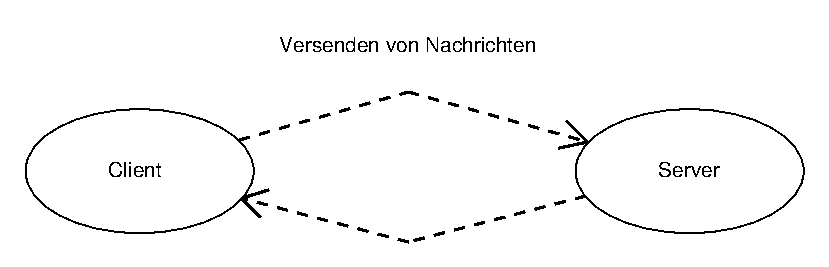
\includegraphics{images/client-server}}
	\caption{Client/Server Modell}
	\label{fig:ClientServer}
\end{figure}

Der Simulator basiert auf dem Client/Server-Prinzip. Jede Simulation besteht in der Regel aus einen teilnehmenden Client und einen Server, die miteinander �ber Nachrichten kommunizieren (s. Abb. \ref{fig:ClientServer}.). Bei komplexen Simulationen k�nnen auch mehrere Clients und/oder Server mitwirken. 

\subsubsection{Prozesse und deren Rollen}

Ein verteiltes System wird anhand von Prozessen simuliert. Jeder Prozess nimmt hierbei eine oder mehrere Rollen ein. Beispielsweise kann ein Prozess die Rolle eines Clients einnehmen und ein weiterer Prozess die Rolle eines Servers. Die M\"{o}glichkeit einem Prozess die Client- und Serverrolle gleichzeitig zuzuweisen ist ebenso gegeben. Ein Prozess k\"{o}nnte auch die Rollen mehrerer Server und Clients gleichzeitig einnehmen. Um einen Prozess zu kennzeichnen, besitzt jeder eine \textbf{eindeutige} Prozess-Identifikationsnummer (PID). 

\subsubsection{Nachrichten}

In einem verteilten System m�ssen Nachrichten verschickt werden k�nnen. Eine Nachricht kann von einem Client- oder Serverprozess verschickt werden und kann beliebig viele Empf�nger haben. Der Inhalt einer Nachricht h�ngt vom verwendeten Protokoll ab. Was unter einem Protokoll zu verstehen ist, wird sp�ter behandelt. Um eine Nachricht zu kennzeichnen, besitzt jede Nachricht eine \textbf{eindeutige} Nachrichten-Identifikationsnummer (NID).

\subsubsection{Lokale und globale Uhren}

In einer Simulation gibt es \textbf{genau eine} globale Uhr. Sie stellt die aktuelle und \textbf{immer korrekte} Zeit dar. Eine globale Uhr geht nie falsch.

Zudem besitzt jeder beteiligte Prozess eine eigene lokale Uhr. Sie stellt die aktuelle Zeit des jeweiligen Prozesses dar. Im Gegensatz zu der globalen Uhr k�nnen lokale Uhren eine falsche Zeit anzeigen. Wenn die Prozesszeit nicht global-korrekt ist (nicht der globalen Zeit gleicht, bzw. eine falsche Zeit anzeigt), dann wurde sie entweder im Laufe einer Simulation neu gestellt, oder sie geht wegen einer Uhrabweichung falsch. Die Uhrabweichung gibt an, um welchen Faktor die Uhr falsch geht. Hierauf wird sp�ter genauer eingegangen. 

\begin{figure}[htbp]
	\centering
	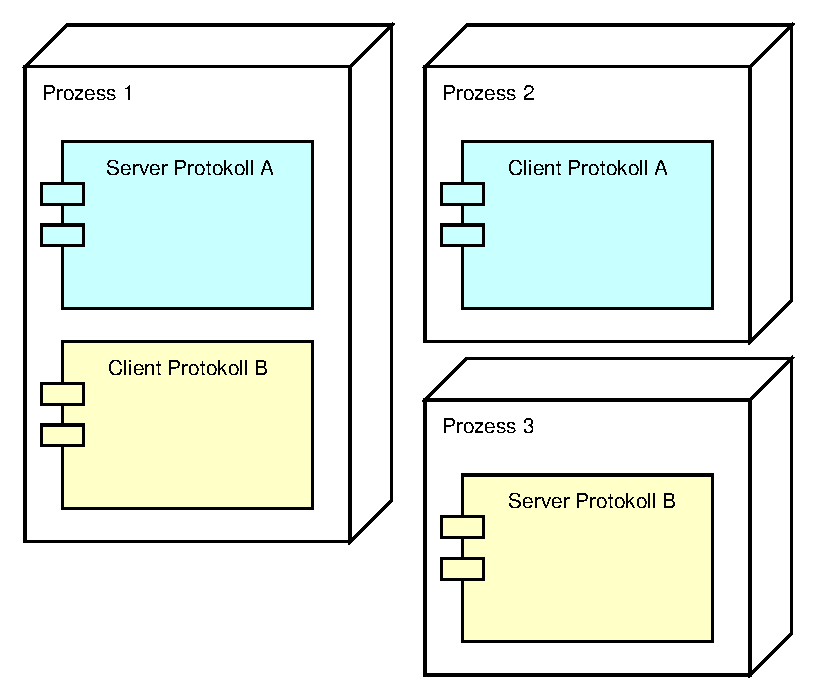
\includegraphics{images/client-server-protokolle}
	\caption{Client/Server Protokolle}
	\label{fig:ClientServerProtokolle}
\end{figure}

Neben den normalen Uhren sind auch die Vektor-Zeitstempel sowie die logischen Uhren von Lamport von Interesse. F�r die Vektor- und Lamportzeiten gibt es hier, im Gegensatz zu der normalen Zeit, keine globalen �quivalente. Konkrete Beispiele zu den Lamport- und Vektorzeiten werden sp�ter in Kapitel 3.11.1. behandelt.

\subsubsection{Ereignisse}

Eine Simulation besteht aus der Hintereinanderausf�hrung von endlich vielen Ereignissen. Beispielsweise kann es ein Ereignis geben, welches einen Prozess eine Nachricht verschicken l�sst. Denkbar w�re auch ein Prozessabsturzereignis. Jedes Ereignis tritt zu einem bestimmten Zeitpunkt ein. Ereignisse mit selber Eintrittszeit werden vom Simulator direkt hintereinander ausgef�hrt. Den Anwender des Simulators hindert dies jedoch nicht, da Ereignisse aus ihrer Sicht parallel ausgef�hrt werden.

\subsubsection{Protokolle}

Eine Simulation besteht auch aus der Anwendung von Protokollen. Es wurde bereits erw�hnt, dass ein Prozess die Rollen von Servern und/oder Clients annehmen kann. Bei jeder Server- und Clientrolle muss zus�tzlich das dazugeh�rige Protokoll spezifiziert werden. Ein Protokoll definiert, wie ein Client und ein Server Nachrichten verschickt, und wie bei Ankunft einer Nachricht reagiert wird. Ein Protokoll legt auch fest, welche Daten in einer Nachricht enthalten sind. Ein Prozess verarbeitet eine empfangene Nachricht nur, wenn er das jeweilige Protokoll versteht.

In Abbildung \ref{fig:ClientServerProtokolle}. sind 3 Prozesse dargestellt. Prozess 1 unterst�tzt serverseitig das Protokoll ``A'' und clientseitig das Protokoll ``B''. Prozess 2 unterst�tzt clientseitig das Protokoll ``A'' und Prozess 3 serverseitig das Protokoll ``B''. Das hei�t, dass Prozess 1 mit Prozess 2 via Protokoll ``A'' und mit Prozess 3 via Protokoll ``B'' kommunizieren kann. Die Prozesse 2 und 3 sind zueinander inkompatibel und k�nnen voneinander erhaltene Nachrichten nicht verarbeiten.

Clients k�nnen nicht mit Clients, und Server nicht mit Servern kommunizieren. F�r eine Kommunikation wird stets mindestens ein Client und ein Server ben�tigt. Diese Einschr�nkung kann aber umgangen werden, indem Prozesse ein gegebenes Protokoll sowohl server- als auch clientseitig unterst�tzen (vgl. Broadcast Protokoll in Kap. 3.3.). 


\chapter{Der Simulator}

\section{Die grafische Benutzerschnittstelle}

\begin{figure}[htbp]
	\centering
	\fbox{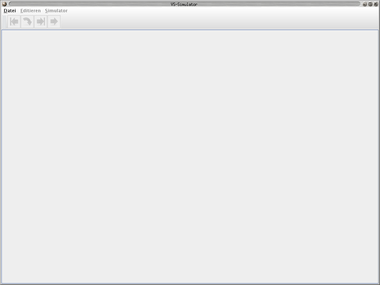
\includegraphics{images/ss-neues-fenster-klein}}
	\caption{Der Simulator nach dem ersten Starten}
	\label{fig:NeuesFenster}
\end{figure}

Der Simulator pr\"{a}sentiert sich nach dem ersten Starten wie in Abbildung \ref{fig:NeuesFenster}. F\"{u}r die Erstellung einer neuen Simulation wird im Men\"{u} ``Datei'' (Abbildung \ref{fig:DateiMenue}) der Punkt ``Neue Simulation'' ausgew\"{a}hlt, wo anschlie�end das Einstellungsfenster f\"{u}r die neue Simulation erscheint.  Auf die einzelnen Optionen wird sp\"{a}ter genauer eingegangen und es werden nun nur die Standardeinstellungen \"{u}bernommen. Die GUI mit einer frischen Simulation sieht dann wie in Abbildung \ref{fig:NeuErstellteSimulation} aus.

\begin{figure}[htbp]
	\centering
	\fbox{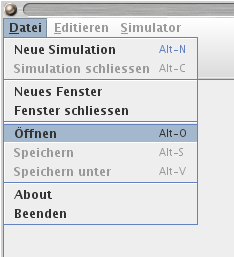
\includegraphics[width=14cm]{images/ss-datei-menu}}
	\caption{Datei-Men\"{u}}
	\label{fig:DateiMenue}
\end{figure}

\subsubsection{Die Men\"{u}zeile}

Im Datei-Men\"{u} (Abbildung \ref{fig:DateiMenue}) lassen sich neue Simulationen erstellen oder die aktuell ge\"{o}ffnete Simulation schlie�en. Neue Simulationen \"{o}ffnen sich standardm\"{a}�ig in einem neuen Tab. Es k\"{o}nnen allerdings auch neue Simulationsfenster, die wiederum eigene Tabs besitzen, ge\"{o}ffnet oder geschlossen werden. In jedem Tab befindet sich eine von den Anderen vollst\"{a}ndig unabh\"{a}ngige Simulation. Es k\"{o}nnen somit beliebig viele Simulationen parallel ausgef\"{u}hrt werden. Die Men\"{u}eintr\"{a}ge ``\"{O}ffnen'', ``Speichern'' und ``Speichern unter'' dienen f\"{u}r das Laden und Speichern von Simulationen. 

\begin{figure}[htbp]
	\centering
	\fbox{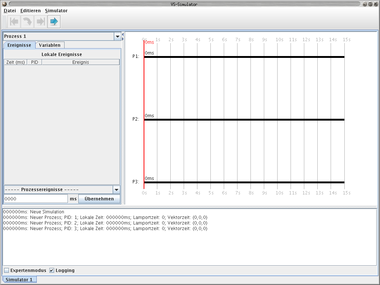
\includegraphics{images/ss-neue-simulation-klein}}
	\caption{Eine neue Simulation}
	\label{fig:NeuErstellteSimulation}
\end{figure}

\"{U}ber das Editieren-Men\"{u} gelangt der Benutzer zu den Simulationseinstellungen, worauf sp\"{a}ter genauer eingegangen wird. Es werden in diesem Men\"{u} auch alle beteiligten Prozesse zum Editieren aufgelistet. W\"{a}hlt der Benutzer dort einen Prozess aus, dann \"{o}ffnet sich der dazugeh\"{o}rige Prozesseditor. Auf diesen wird ebenso sp\"{a}ter genauer eingegangen. Das Simulator-Men\"{u} bietet die selben Optionen wie die Toolbar, welche im n\"{a}chsten Teilkapitel beschrieben wird.

Einige Men\"{u}unterpunkte sind erst erreichbar, wenn im aktuellen Fenster bereits eine Simulation erstellt oder geladen wurde.

\subsubsection{Die Toolbar}

Oben links im Simulator befindet sich die Toolbar (Abbildung \ref{fig:Toolbar}). Die Toolbar enth\"{a}lt die Funktionen, die vom Benutzer am h\"{a}ufigsten ben\"{o}tigt werden.

\begin{figure}[htbp]
	\centering
	\fbox{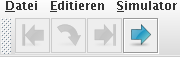
\includegraphics[width=5cm]{images/ss-neue-simulation-toolbar}}
	\caption{Die Men\"{u}zeile inklusive Toolbar}
	\label{fig:Toolbar}
\end{figure}

Die Toolbar bietet vier verschiedene Funktionalit\"{a}ten an:

\begin{itemize}
	%\setlength{\itemsep}{-1mm}
	\item Starten der Simulation; kann nur bet\"{a}tigt werden, wenn die Simulation derzeit nicht l\"{a}uft.
	\item Pausieren der Simulation, kann nur bet\"{a}tigt werden, wenn die Simulation derzeit l\"{a}uft.
	\item Wiederholen der Simulation, kann nicht bet\"{a}tigt werden, wenn die Simulation noch nicht gestartet wurde. 
	\item Zur\"{u}cksetzen der Simulation, kann nur bet\"{a}tigt werden, wenn die Simulation pausiert wurde oder wenn die Simulation abgelaufen ist.
\end{itemize}

Die Toolbar l\"{a}sst sich auch nach Belieben repositionieren (z.B. links, rechts oder unten des Simulatorfensters). Hierf\"{u}r muss sie per ``Drag-n-Drop'' zur Zielposition gezogen werden.

\subsubsection{Die Visualisierung}

\begin{figure}[htbp]
	\centering
	\fbox{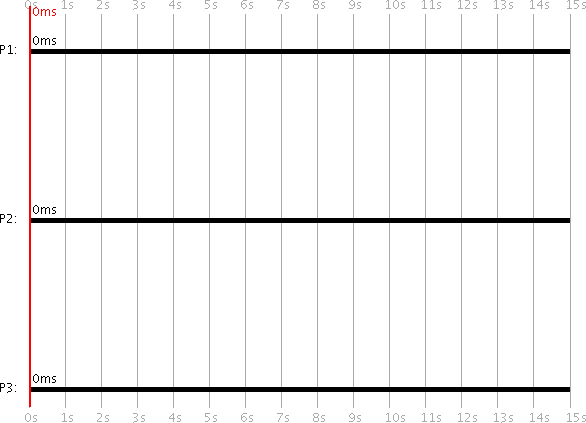
\includegraphics[width=14cm]{images/ss-visualisierung}}
	\caption{Visualisierung einer noch nicht gestarteten Simulation}
	\label{fig:Visualisierung}
\end{figure}

Mittig rechts in Abbildung \ref{fig:NeuErstellteSimulation} befindet sich die grafische Repr\"{a}sentation der Simulation. Die X-Achse gibt die Zeit in Millisekunden an. Unsere Demo-Simulation endet nach genau 15 Sekunden. In Abbildung \ref{fig:Visualisierung} sind 3 Prozesse (mit den PIDs 1, 2 und 3) dargestellt, die jeweils einen eigenen horizontalen schwarzen Balken besitzen. Auf diesen Prozessbalken kann der Benutzer die jeweilige lokale Prozesszeit ablesen. Die vertikale rote Linie stellt die globale Simulationszeit dar. 

Die Prozessbalken dienen auch f\"{u}r Start- und Zielpunkte von Nachrichten. Wenn beispielsweise Prozess 1 eine Nachricht an Prozess 2 verschickt, so wird eine Linie vom einen Prozessbalken zum Anderen gezeichnet. Nachrichten, die ein Prozess an sich selbst schickt, werden nicht visualisiert. Sie werden aber im Loggfenster (mehr dazu sp\"{a}ter) protokolliert.

Eine andere M\"{o}glichkeit einen Prozesseditor aufzurufen ist ein Linksklick auf den zum Prozess geh\"{o}rigen Prozessbalken. Dies muss also nicht zwingend \"{u}ber das Simulator-Men\"{u} geschehen. Ein Rechtsklick hingegen \"{o}ffnet ein Popup-Fenster mit weiteren Auswahlm\"{o}glichkeiten (Abbildung \ref{fig:RechtsklickProzessbalken}). Ein Prozess kann \"{u}ber das Popup-Men\"{u} nur dann abst\"{u}rzen oder wiederbelebt werden, wenn die Simulation aktuell l\"{a}uft.

\begin{figure}[htbp]
	\centering
	\fbox{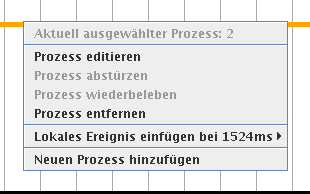
\includegraphics[width=8.8cm]{images/ss-rechtsklick-prozessbalken}}
	\caption{Rechtsklick auf einen Prozessbalken}
	\label{fig:RechtsklickProzessbalken}
\end{figure}

Generell kann die Anzahl der Prozesse nach belieben variieren. Die Dauer der Simulation betr\"{a}gt mindestens 5 -und maximal 120 Sekunden. Die Simulation endet erst, wenn die globale Zeit 15 Sekunden erreicht hat, und nicht, wenn eine lokale Prozesszeit die 15 Sekunden erreicht.

\subsubsection{Farbliche Differenzierung}

Farben helfen dabei die Vorg\"{a}nge einer Simulation zu deuten. Standardm\"{a}�ig werden die Prozesse (Prozessbalken) und Nachrichten mit den Farben wie in Tabelle \ref{tb:Farben} aufgelistet dargestellt. Dies sind lediglich die Standarfarben, welche \"{u}ber die Einstellungen umkonfigurierbar sind.

\begin{table}
	\fbox{
	\begin{tabular}{c|l}
		\textbf{Prozessfarbe} & \textbf{Bedeutung} \\
		\hline 
		 	Schwarz & Simulation l\"{a}uft derzeit nicht (z.B. noch nicht gestartet, abgelaufen oder\\
				& pausiert)\\
		 	Orange & Die Maus befindet sich \"{u}ber den Prozessbalken\\
		 	Rot & Der Prozess ist abgest\"{u}rzt\\
			& \\
		\textbf{Nachrichtenfarbe} & \textbf{Bedeutung} \\
		\hline 
		 	Gr\"{u}n & Die Nachricht ist noch unterwegs und hat das Ziel noch nicht erreicht\\
		 	Blau & Die Nachricht hat das Ziel erfolgreich erreicht\\
		 	Rot & Die Nachricht ging verloren (entweder weil der Zielprozess abgest\"{u}rzt ist\\
				& oder weil sie unterwegs verloren ging)\\

	\end{tabular}\\
	}
	\caption{Farbliche Differenzierung von Prozessen und Nachrichten}
	\label{tb:Farben}
\end{table}

\subsubsection{Die Sidebar}

Mithilfe der Sidebar lassen sich Prozessereignisse programmieren. Ganz oben in Abbildung \ref{fig:Sidebar} ist der zu verwaltende Prozess selektiert (hier mit der PID 1). In dieser Prozessauswahl gibt es auch die M\"{o}glichkeit ``Alle Prozesse'' auszuw\"{a}hlen, womit die Ereignisse aller Prozesse gleichzeitig verwaltet werden k\"{o}nnen. Unter ``Lokale Ereignisse'' versteht der Benutzer diejenigen Ereignisse, die auftreten, wenn eine bestimmte lokale Zeit des dazugeh\"{o}rigen Prozesses eingetreten ist. Die darunterliegende Ereignistabelle listet alle programmierten Ereignisse (hier noch keine vorhanden) mitsamt Eintrittszeiten sowie den PIDs auf.

\begin{figure}[htbp]
	\centering
	\fbox{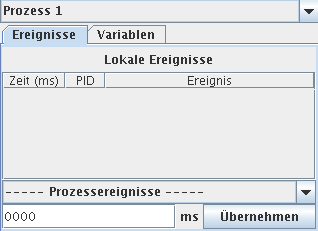
\includegraphics[width=9cm]{images/ss-sidebar}}
	\caption{Die Sidebar mit leerem Ereigniseditor}
	\label{fig:Sidebar}
\end{figure}

F\"{u}r die Erstellung eines neuen Ereignisses kann der Benutzer entweder mit einem Rechtsklick auf einen Prozessbalken (Abbildung \ref{fig:RechtsklickProzessbalken}) klicken, oder unterhalb der Ereignistabelle ein Ereignis ausw\"{a}hlen (Abbildung \ref{fig:Ereignisauswahl}), im darunter liegendem Textfeld die Zeit eintragen und auf ``\"{U}bernehmen'' klicken. Beispielsweise wurden auf Abbildung \ref{fig:SidebarMitEreignissen} drei Ereignisse hinzugef\"{u}gt: Absturz nach 123ms, Wiederbelebung nach 321ms und erneuter Absturz nach 3000ms des Prozesses mit der ID 1. 

\begin{figure}[htbp]
	\centering
	\fbox{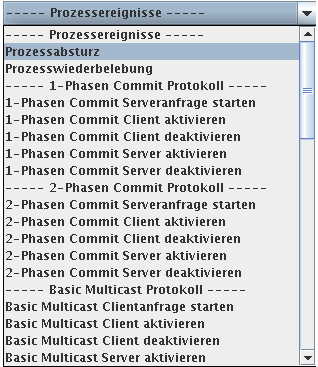
\includegraphics[width=9cm]{images/ss-ereignisauswahl}}
	\caption{Die Ereignisauswahl via Sidebar}
	\label{fig:Ereignisauswahl}
\end{figure}

Mit einem Rechtsklick auf den Ereigniseditor lassen sich alle selektierten Ereignisse entweder kopieren oder l\"{o}schen. Mithilfe der Strg-Taste k\"{o}nnen auch mehrere Ereignisse gleichzeitig markiert werden. Die Eintr\"{a}ge der Spalten f\"{u}r die Zeit und der PID lassen sich nachtr\"{a}glich editieren. Somit besteht eine komfortable M\"{o}glichkeit bereits programmierte Ereignisse auf eine andere Zeit zu verschieben oder einem anderen Prozess zuzuweisen.

In der Sidebar gibt es neben dem Ereignis-Tab einen weiteren Tab ``Variablen''. Hinter diesem Tab verbirgt sich der Prozesseditor des aktuell ausgew\"{a}hlten Prozesses. Dort k\"{o}nnen alle Variablen des Prozesses editiert werden. Der Prozesseditor wird sp\"{a}ter genauer behandelt. 

\begin{figure}[htbp]
	\centering
	\fbox{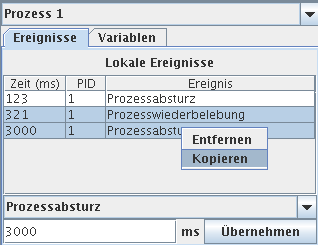
\includegraphics[width=9cm]{images/ss-sidebar-mit-ereignissen}}
	\caption{Der Ereigniseditor mit 3 programmierten Ereignissen}
	\label{fig:SidebarMitEreignissen}
\end{figure}

\subsubsection{Das Loggfenster}

Das Loggfenster (Abbildung \ref{fig:NeuErstellteSimulation}, unten) protokolliert  in chronologischer Reihenfolge alle eingetroffenen Ereignisse. Auf Abbildung \ref{fig:Loggfenster} sieht der Benutzer das Loggfenster nach Erstellung unserer Simulation, an welcher 3 Prozesse beteiligt sind. Am Anfang eines Loggeintrages wird stets die globale Zeit in Millisekunden protokolliert. Bei jedem Prozess werden ebenso seine lokale Zeiten sowie die Lamport- und die Vektor-Zeitstempel aufgef\"{u}hrt. Letztere werden sp\"{a}ter genauer behandelt.  Hinter den Zeitangaben werden weitere Angaben, wie beispielsweise welche Nachricht mit welchem Inhalt verschickt wurde und welchem Protokoll sie angeh\"{o}rt, gemacht. Dies wird sp\"{a}ter noch anhand von Beispielen demonstriert.

\begin{figure}[htbp]
	\centering
	\fbox{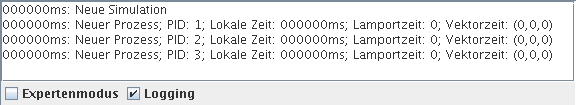
\includegraphics[width=16.5cm]{images/ss-loggfenster}}
	\caption{Das Loggfenster}
	\label{fig:Loggfenster}
\end{figure}

Mit dem Deaktivieren der Checkbox ``Logging'' l\"{a}�t sich das Loggen von Nachrichten tempor\"{a}r deaktivieren. Mit deaktivierter Logging-Checkbox werden keine neuen Nachrichten mehr ins Loggfenster geschrieben. Nach Reaktivieren der Checkbox werden alle ausgelassenen Nachrichten nachtr\"{a}glich in das Fenster geschrieben. Ein deaktiviertes Loggen kann zu verbessertem Leistungsverhalten des Simulators f\"{u}hren (z.B. kein Rucklen; ist vom verwendeten Computer, auf dem der Simulator l\"{a}uft, abh\"{a}ngig). Dieser Umstand ist der sehr langsamen Java-Implementierung der JTextArea-Klasse zu verdanken, die schnelle Updates nur sehr tr\"{a}ge durchf\"{u}hrt.

\"{U}ber die Checkbox ``Expertenmodus'' wird der Expertenmodus aktiviert beziehungsweise deaktiviert. 

\section{Der Expertenmodus}

\begin{figure}[htbp]
	\centering
	\fbox{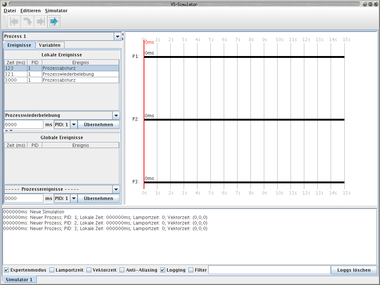
\includegraphics{images/ss-simulation-expertenmodus-klein}}
	\caption{Der Simulator im Expertenmodus}
	\label{fig:SimulationExpertenmodus}
\end{figure}

Der Simulator kann in zwei verschiedenen Modi betrieben werden. Es gibt einen einfachen- und einen Expertenmodus. Der Simulator startet standardm\"{a}�ig im einfachen Modus, sodass sich der Benutzer nicht mit der vollen Funktionalit\"{a}t des Simulators auf einmal auseinandersetzen mu�. Der einfache Modus ist \"{u}bersichtlicher, bietet jedoch weniger Funktionen an. Der Expertenmodus eignet sich f\"{u}r mehr erfahrene Anwender und bietet dementsprechend auch mehr Flexibilit\"{a}t. Der Expertenmodus kann \"{u}ber die gleichnamige Checkbox unterhalb des Loggfensters oder \"{u}ber die Simulationseinstellungen aktiviert oder deaktiviert werden.  Auf Abbildung \ref{fig:SimulationExpertenmodus} ist der Simulator im Expertenmodus zu sehen. Wenn der Benutzer den Simulator im Expertenmodus mit Abbildung \ref{fig:NeuErstellteSimulation} vergleicht, dann fallen einige Unterschiede auf, die nun behandelt werden.

\begin{figure}[htbp]
	\centering
	\fbox{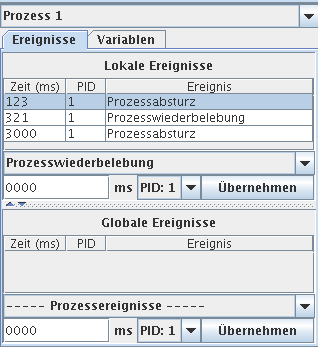
\includegraphics[width=9cm]{images/ss-sidebar-expertenmodus}}
	\caption{Die Sidebar im Expertenmodus}
	\label{fig:SidebarExpertenmodus}
\end{figure}

Der erste Unterschied ist in der Sidebar erkennbar (Abbildung \ref{fig:SidebarExpertenmodus}). Dort sind nun, zus\"{a}tzlich den lokalen Ereignissen, auch globale Ereignisse editierbar.  Wie bereits erw\"{a}hnt, sind unter lokale Ereignisse diejenigen Ereignisse zu verstehen, die auftreten, wenn eine bestimmte lokale Zeit des dazugeh\"{o}rigen Prozesses eingetreten ist. Globale Ereignisse hingegen sind diejenigen Ereignisse, die auftreten, wenn eine bestimmte globale Zeit eingetreten ist. Ein globales Ereignis nimmt die globale Zeit- und ein lokales Ereignis die lokale Prozesszeit als Eintrittskriterium. Globale Ereignisse machen somit nur einen Unterschied, wenn sich die lokalen Prozesszeiten von der globalen Zeit unterscheiden.

Eine weitere neue Funktionalit\"{a}t ist die M\"{o}glichkeit einem neuzuerstellenen Ereignis die PID direkt zuzuweisen. Im einfachen Modus wurde, wenn der Benutzer ein neues Ereignis erstellte, standardm\"{a}�ig immer die PID des aktuell (in der obersten Combo-Box) ausgew\"{a}hlten Prozesses verwendet. In dieser Combo-Box sollte der Benutzer gegebenenfalls ``Alle Prozesse'' selektieren, damit im Ereigniseditor stets die Ereignisse aller Prozesse aufgelistet werden.

Weitere Unterschiede machen sich unterhalb des Loggfensters bemerkbar. Dort gibt es unter Anderem zwei neue Checkboxen ``Lamportzeit'' und ``Vektorzeit''.  Aktiviert der Benutzer eine dieser beiden Checkboxen, dann wird die Lamport- beziehungsweise Vektorzeit in die Visualisierung dargestellt. \"{U}bersichtshalber kann der Benutzer nur jeweils eine dieser beiden Checkboxen aktivieren. Wenn die Lamportzeit-Checkbox bereits aktiviert ist und der Benutzer versucht die Vektorzeit-Checkbox zus\"{a}tzlich zu aktivieren, so wird die Lamportzeit-Checkbox automatisch deaktiviert und virce versa. 

Die Anti-Aliasing-Checkbox erm\"{o}glicht dem Benutzer Anti-Aliasing zu aktivieren und deaktivieren. Mit aktiviertem Anti-Aliasing werden alle Grafiken der Visualisierung gerundet dargestellt. Aus Performancegr\"{u}nden ist Anti-Aliasing standardm\"{a}�ig deaktiviert.

Je komplexer eine Simulation wird, desto un\"{u}bersichtlicher werden die Eintr\"{a}ge im Loggfenster. Hier f\"{a}llt es zunehmend schwerer die \"{U}bersicht aller Ereignisse zu behalten. Um dem entgegenzuwirken gibt es im Expertenmodus einen Loggfilter, welcher es erm\"{o}glicht nur die wesentlichen Daten aus den Loggs zu filtern. Der Loggfilter wird anhand der dazugeh\"{o}rigen Checkbox ``Filter'' aktiviert beziehungsweise deaktiviert. In der dahinterliegenden Eingabezeile kann ein regul\"{a}rer Ausdruck in Java-Syntax angegeben werden. Beispielsweise werden mit ``\texttt{PID: (1|2)}'' nur Loggzeilen angezeigt, die entweder ``\texttt{PID: 1}'' oder ``\texttt{PID: 2}'' beinhalten. Alle anderen Zeilen, beispielsweise mit ``\texttt{PID: 3}'', werden dabei nicht angezeigt. Mit aktiviertem Loggfilter werden nur die Loggzeilen angezeigt, auf die der regul\"{a}re Ausdruck passt. Der Loggfilter kann auch nachtr\"{a}glich aktiviert werden. Bereits protokollierte Ereignisse werden jedes Mal erneut gefiltert. Der Loggfilter kann auch w\"{a}hrend einer laufenden Simulation verwendet werden. Wenn der Loggfilter deaktiviert wird, dann werden wieder alle Nachrichten (auch nachtr\"{a}glich) im Loggfenster angezeigt. 

\section{Ereignisse}

Es wird zwischen zwei verschiedenen Haupttypen von Ereignissen unterschieden: Programmierbare Ereignisse und nicht-programmierbare Ereignisse. Programmierbare Ereignisse lassen sich im Ereigniseditor editieren und deren Eintrittszeiten h\"{a}ngen von den lokalen Prozessuhren oder der globalen Uhr ab. Nicht-programmierbare Ereignisse lassen sich hingegen nicht im Ereigniseditor angeben und treten nicht wegen einer bestimmten Uhrzeit ein, sondern aufgrund anderer Gegebenheiten wie in etwa das Eintreffen einer Nachricht oder das Ausf\"{u}hren einer Aktion aufgrund eines Weckers, worauf weiter unten nochmal genauer eingegangen wird.

\subsubsection{Prozessabsturz- und Wiederbelebung (programmierbar)}

Die beiden grundliegensten Ereignisse sind ``Prozessabsturz'' sowie ``Prozesswiederbelebung''. Wenn ein Prozess abgest\"{u}rzt ist, so wird sein Prozessbalken in rot dargestellt. Ein abgest\"{u}rzter Prozess kann keine weiteren Ereignisse mehr verarbeiten und, wenn er eine Nachricht empfangen sollte, geht diese verloren. Die einzige Ausnahme bildet ein Wiederbelebungsereignis. Ein abgest\"{u}rzter Prozess kann nichts, au�er wiederbelebt werden. W\"{a}hrend eines Prozessabsturzes l\"{a}uft die lokale Prozessuhr, abgesehen der Lamport- und Vektor-Uhren, wie gewohnt weiter. D.h. es k\"{o}nnte sein, dass ein Prozess einige seiner Ereignisse gar nicht ausf\"{u}hrt, da er zu den Ereigniseintrittszeiten abgest\"{u}rzt ist. Wenn im echten Leben ein Computer abst\"{u}rzt oder abgeschaltet wird, dann l\"{a}uft dort die Hardware-Uhr, unabh\"{a}ngig vom Betriebssystem, auch weiter.

\subsubsection{Aktivierung und Deaktivierung von Protokollen sowie Starten von Anfragen (programmierbar)}
Wir wissen bereits, dass ein Prozess mehrere Protokolle Client- und auch Serverseitig unterst\"{u}tzen kann. Welches Protokoll von einem Prozess unterst\"{u}tzt wird, kann der Benutzer anhand von Protokollaktivierungs- und Protokolldeaktivierungsereignissen konfigurieren. Somit besteht die M\"{o}glichkeit, dass ein gegebener Prozess ein bestimmtes Protokoll erst zu einem bestimmten Zeitpunkt unterst\"{u}tzt und gegebenenfalls ein anderes Protokoll abl\"{o}st. Jedes Protokoll kann entweder Server- oder Clientseitig aktiviert beziehungsweise deaktiviert werden. Welche Protokolle es gibt wird sp\"{a}ter behandelt. Der Benutzer hat die Auswahl zwischen f\"{u}nf verschiedenen Protokollereignistypen: 

\begin{itemize}
	\item Aktivierung des Clients eines gegebenen Protokolls
	\item Aktivierung des Servers eines gegebenen Protokolls
	\item Deaktivierung des Clients eines gegebenen Protokolls
	\item Deaktivierung des Servers eines gegebenen Protokolls
	\item Starten einer Client/Server-Anfrage eines gegebenen Protokolls
\end{itemize}

Ob sich das Ereignis f\"{u}r das Starten einer Anfrage auf einen Client oder einen Server bezieht h\"{a}ngt vom verwendeten Protokoll ab. Es gibt Protokolle, wo der Client die initiale Anfrage starten muss, und es gibt Protokolle, wo der Server diese Aufgabe \"{u}bernimmt. Beispielsweise startet bei dem ``Ping-Pong Protokoll'' der Client- und bei dem ``Commit-Protokollen'' der Server immer die erste Anfrage. Es gibt kein Protokoll, wo Client und Server jeweils eine initiale Anfragen starten k\"{o}nnen. 

Bei allen dieser f\"{u}nf Ereignissen kann der betroffene Prozess noch beliebig andere Dinge, abh\"{a}ngig vom Protokoll, tun. Beispielsweise kann er den Inhalt der Nachricht generieren oder lokale Variablen initialisieren oder eine der lokalen Uhzeiten \"{a}ndern oder Wecker f\"{u}r ``Callback Ereignisse'' setzen (mehr dazu sp\"{a}ter).

\subsubsection{Nachrichtenempfang sowie Antwortnachrichten (nicht-programmierbar)}

Nachdem ein Prozess eine Nachricht empf\"{a}ngt wird zuerst \"{u}berpr\"{u}ft ob er das dazugeh\"{o}rige Protokoll unterst\"{u}tzt. Wenn der Prozess das Protokoll unterst\"{u}tzt, wird geschaut ob es sich um eine Client- oder eine Servernachricht handelt. Wenn es sich um eine Clientnachricht handelt, so mu� der Empf\"{a}ngerprozess ein das Protokoll serverseitig unterst\"{u}tzen und virce versa. Wenn alles passt, dann f\"{u}hrt der Empf\"{a}ngerprozess die vom Protokoll definierten Aktionen aus. In der Regel berechnet der Prozess irgendeinen Wert und schickt ihn \"{u}ber eine Antwortnachricht zur\"{u}ck. Es k\"{o}nnen aber auch beliebig andere Aktionen ausgef\"{u}hrt werden. Welche dies sind h\"{a}ngt wieder vom Protokoll ab.

\subsubsection{Callback-Ereignisse (nicht-programmierbar)}

Ein Callback-Ereignis kann von einem Protokoll ausgel\"{o}st werden. Das Protokoll setzt einen Wecker, der angibt zur welcher lokalen Uhrzeit eine weitere Aktion ausgef\"{u}hrt werden soll. Zum Beispiel lassen sich hiermit Timeouts realisieren: Wenn ein Protokoll eine Antwort erwartet, diese aber nicht eintrifft, dann kann nach einer bestimmten Zeit eine Anfrage erneut verschickt werden! Es k\"{o}nnen beliebig viele Callback-Ereignisse definiert werden. Wenn sie noch nicht ausgef\"{u}hrt wurden und aufgrund eines anderen Ereignisses nicht mehr ben\"{o}tigt werden, k\"{o}nnen sie vom Protokoll auch wieder entfernt werden. Wenn ein Callback-Ereignis ausgef\"{u}hrt wird, kann es sich selbst wieder f\"{u}r eine weitere Ausf\"{u}hrung erneut planen. So lassen sich periodisch wieder-eintreffende Ereignisse realisieren. Beispielsweise verwenden die ``Commit-Protokolle'' (mehr dazu sp\"{a}ter) Callback-Ereignisse, indem solange Anfragen verschickt werden, bis alle ben\"{o}tigten Antworten vorliegen.

\subsubsection{Zufallsereignisse (nicht-programmierbar)}

Die Eintrittszeit eines Zufallsereignisses wird vom Simulator zuf\"{a}llig gew\"{a}hlt. Es besteht lediglich die M\"{o}glichkeit die Zuf\"{a}lligkeit anhand einer Wahrscheinlichkeit, dass das Ereignis \"{u}berhaupt eintritt, einzustellen. Ein Beispiel ist ein zuf\"{a}lliger Prozessabsturz, dessen Wahrscheinlichkeit unter den Prozessvariablen konfiguriert werden kann. Diese Variable wird im Abschnitt \"{u}ber Prozessvariablen noch ausf\"{u}hrlicher beschrieben.


\section{Einstellungen}

In diesem Abschnitt wird auf die m\"{o}glichen Konfigurationsm\"{o}glichkeiten genauer eingegangen. Es wird zwischen drei verschiedenen Typen von Einstellungen unterschieden. Zun\"{a}chst gibt es globale Simulationseinstellungen. Diese beinhalten Variablen die die gesamte Simulation betreffen. Zudem hat jeder Prozess seine eigenen lokale Einstellungen. Dar\"{u}berhinaus kann jedes Protokoll f\"{u}r jeden Prozess separat eingestellt werden. 

\subsection{Variablendatentypen}

\begin{table}
	\centering
	\fbox{
	\begin{tabular}{l|l}
		\textbf{Prefix} & \textbf{Beschreibung}\\
		\hline 
			\texttt{Boolean} & boolschen Wert, z.B. true oder false\\
			\texttt{Color} & Java-Farbobjekt\\
			\texttt{Float} & Flieskommazahl einfacher genauigkeit\\
			\texttt{Integer} & Einfache Integerzahl\\
			\texttt{Integer[]} & Integervektor\\
			\texttt{Long} & Einfache Long-Zahl\\
	\end{tabular}
	}
	\caption{Verf\"{u}gbare Datentypen f\"{u}r editierbare Variablen}
	\label{tb:VariablenDatentypen}
\end{table}

Der Simulator unterscheidet zwischen mehreren Datentypen, in denen die einstellbaren Variablen vorliegen k\"{o}nnen (Tabelle \ref{tb:VariablenDatentypen}). Im folgenden bedeutet (\texttt{Prefix}: \textit{wert}), dass die Variable vom Typ \texttt{Prefix} ist, und standardm\"{a}ssig den Wert \textit{wert} zugewiesen hat. Lediglich die Variablenwerte, jedoch nicht die Variablentypen sowie Variablennamen, lassen sich vom Benutzer \"{a}ndern.

\subsection{Simulationseinstellungen}

\begin{figure}[htbp]
	\centering
	\fbox{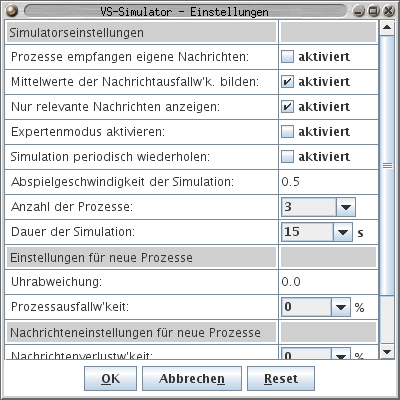
\includegraphics{images/ss-simulationseinstellungen}}
	%\fbox{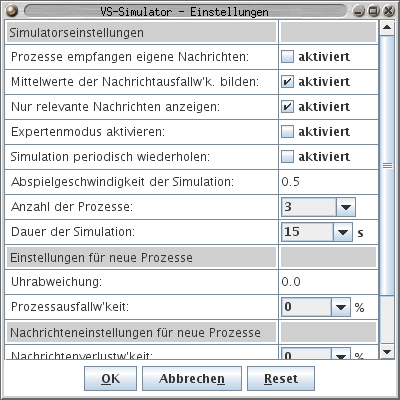
\includegraphics[width=11cm]{images/ss-simulationseinstellungen}}
	\caption{Das Fenster zu den Simulationseinstellungen}
	\label{fig:Simulationseinstellungen}
\end{figure}

Beim Erstellen einer neuen Simulation erscheint zun\"{a}chst das dazugeh\"{o}rige Einstellungsfenster (Abbildung \ref{fig:Simulationseinstellungen}). In der Regel reicht es, wenn der Benutzer hier die Standardwerte \"{u}bernimmt. Es besteht auch die M\"{o}glichkeit die Einstellungen nachtr\"{a}glich zu editieren, indem das Einstellungsfenster via ``Editieren $\rightarrow$ Einstellungen'' erneut aufgerufen wird.

Im Folgenden werden alle in den Simulationseinstellungen verf\"{u}gbaren Variablen beschrieben. Die Klammern geben den Typen und die Standardwerte an, in denen die Variablen vorliegen. 

\begin{itemize}
	\item \textbf{Prozesse empfangen eigene Nachrichten} \textit{(Boolean: false)}: Standardm\"{a}�ig k\"{o}nnen Prozesse \"{u}bersichtshalber keine Nachrichten empfangen, die sie selbst verschickt haben. Wenn diese Variable jedoch auf true gesetzt wird, dann kann ein Prozess auch auf selbst verschickte Nachrichten antworten. Die Zeit f\"{u}r das Versenden und Empfangen einer Nachricht an sich selbst betr\"{a}gt jedoch stets 0ms. Diese Variable sollte mit Vorsicht verwendet werden, da hierdurch, bedingt aus den 0ms, Endlosschleifen entstehen k\"{o}nnen. 
	\item \textbf{Mittelwerte der Nachrichtenverlustwahrscheinlichkeiten bilden} \textit{(Boolean, true)}: Jede Nachricht die verschickt wird hat, je nach Einstellungen, eine vom verschickendem Prozess abh\"{a}ngige zuf\"{a}llige \"{U}bertragungszeit. Wenn diese Option aktiviert ist, so wird der Mittelwert vom Sende- und Empfangsprozess gebildet. Ansonsten wird stets die \"{U}bertragungszeit, die beim Senderprozesses angegeben wurde, verwendet.
	\item \textbf{Nur relevante Nachrichten anzeigen} \textit{(Boolean: true)}: Wenn nur alle relevanten Nachrichten angezeigt werden, so werden Nachrichten an einen Prozess die er selbst nicht verarbeiten kann, weil er das dazugeh\"{o}rige Protokoll nicht unterst\"{u}tzt, nicht angezeigt. Hierdurch wird eine Simulation viel \"{u}bersichtlicher dargestellt.
	\item \textbf{Expertenmodus aktivieren} \textit{(Boolean, false)}: Hier l\"{a}sst sich der Expertenmodus auf einen alternativen Weg aktivieren beziehungsweise wieder deaktivieren. 
	\item \textbf{Simulation periodisch wiederholen} \textit{(Boolean: false)}: Wenn diese Variable auf true gesetzt ist, so wird die Simulation jedes Mal nach Ablauf automatisch erneut gestartet. 
	\item \textbf{Abspielgeschwindigkeit der Simulation} \textit{(Float: 0.5)}: Gibt den Faktor der Simulationsabspielgeschindigkeit an. Wenn als Faktor 1 gew\"{a}hlt wird, dann dauert eine simulierte Sekunde so lange wie eine Sekunde in echt. Der Faktor 0.5 gibt somit an, dass die Simulation mit halber Echtzeitgschwindigkeit abgespielt wird.
	\item \textbf{Anzahl der Prozesse} \textit{(Integer: 3)}: Gibt an, wie viele Prozesse an der Simulation teilnehmen sollen. Wie schon erw\"{a}hnt kann der Benutzer auch nachtr\"{a}glich via Rechtsklick auf den Prozessbalken den jeweiligen Prozess aus der Simulation entfernen oder weitere Prozesse hinzuf\"{u}gen.
	\item \textbf{Dauer der Simulation} \textit{(Integer: 15)}: Gibt die Dauer der Simulation in Sekunden an.
\end{itemize}

Die weiteren Einstellungen unter ``Einstellungen f\"{u}r neue Prozesse'' sowie ``Nachrichteneinstellungen f\"{u}r neue Prozesse'' geben lediglich Standardwerte an, die f\"{u}r neu zu erstellende Prozesse verwendet werden. Die dort verf\"{u}gbaren Variablen werden im folgenden Teilkapitel genauer beschrieben.

\subsection{Prozess- und Protokolleinstellungen}

Jeder Prozess besitzt folgende Variablen, die entweder via dem Variablen-Tab in der Sidebar oder ``Editieren $\rightarrow$ Prozess \textit{PID}'' oder Linksklick auf den Prozessbalken editiert werden k\"{o}nnen. Das Fenster f\"{u}r die Prozesseinstellungen wird auch als Prozesseditor bezeichnet.

\begin{itemize}
	\item \textbf{Uhrabweichung} \textit{(Float: 0.0)}: Gibt den Faktor $f$ an, um den die lokale Prozessuhr abweicht. Der Faktor 0.0 besagt beispielsweise, dass die Uhr keine Abweichung hat. Ein Faktor von 1 w\"{u}rde hingegen bedeuten, dass die Uhr mit doppelter Geschwindigkeit liefe. F\"{u}r $f$ sind nur Werte $> -1.0$ erlaubt, da sonst die Prozessuhr r\"{u}ckw\"{a}rts laufen k\"{o}nnte. Bei allen anderen Werten wird der Faktor wieder automatisch auf 0.0 gesetzt. Da der Simulator intern mit Flie�kommazahlen doppelter Genauigkeit arbeitet, kann es zu kleinen, jedoch vernachl\"{a}ssigbaren, Rundungsfehlern kommen. 
	\item \textbf{Prozessausfallwahrscheinlichkeit} \textit{(Integer: 0)}: Gibt eine Wahrscheinlichkeit in Prozent an, ob der gegebene Prozess w\"{a}hrend der Simulation zuf\"{a}llig abst\"{u}rzt. Die Wahrscheinlichkeit bezieht sich auf die komplette Simulationsdauer. Bei einer Einstellung von 100 Prozent und der Simulationsdauer von 15 Sekunden st\"{u}rzt der Prozess auf jeden Fall zwischen 0ms und 15000ms ab. An welcher Stelle dies geschieht wird zuf\"{a}llig bestimmt. Wenn der Prozess nach seinem Absturz wiederbelebt wird, st\"{u}rzt er nicht noch einmal zuf\"{a}llig ab. Dies gilt allerdings nicht, wenn die Prozesseinstellungen nach dem Zufallsabsturz erneut ge\"{a}ndert und \"{u}bernommen wurden, da dann das Zufallsabst\"{u}rzereignis erneut erstellt wird. 
	\item \textbf{Lokale Zeit} \textit{(Long: 0)}: Gibt die aktuelle lokale Prozesszeit in Millisekunden an. Es empfiehlt sich daher die Simulation, bevor Prozesseinstellungen vorgenommen werden, zu pausieren. 
	\item \textbf{Nachrichtenverlustwahrscheinlichkeit} \textit{(Integer: 0)}: Gibt eine Wahrscheinlichkeit in Prozent an, ob eine vom aktuell ausgew\"{a}hlten Prozess verschickte Nachricht unterwegs verloren geht. An welcher Stelle die Nachricht zwischen dem Sende- und Empfangsprozess verloren geht wird vom Simulator zuf\"{a}llig gew\"{a}hlt.
	\item \textbf{Maximale \"{U}bertragungszeit} \textit{(Long: 2000)}: Gibt die Dauer in Millisekunden an, die eine vom Prozess verschickte Nachricht maximal ben\"{o}tigt, bis sie einen Empf\"{a}ngerprozess erreicht. Im weiteren Verlauf wird dieser Wert mit $t_{max}$ bezeichnet. Der tats\"{a}chlich verwendete Wert wird zuf\"{a}llig zwischen der minimalen- und der maximalen Zeit (jeweils inklusive) gew\"{a}hlt. 
	\item \textbf{Minimale \"{U}bertragungszeit} \textit{(Long: 500)}: Gibt die Dauer in Millisekunden an, die eine vom Prozess verschickte Nachricht minimal ben\"{o}tigt, bis sie einen Empf\"{a}ngerprozess erreicht. Im weiteren Verlauf wird dieser Wert mit $t_{min}$ bezeichnet. Der tats\"{a}chlich verwendete Wert wird zuf\"{a}llig zwischen der minimalen- und der maximalen Zeit (jeweils inklusive) gew\"{a}hlt. \\
		\\
		Wenn die \"{U}bertragungszeit einer Nachricht immer exakt die selbe Zeit in Anspruch nehmen soll, dann m\"{u}ssen die Prozesseinstellungen mit $t_{min} = t_{max}$ konfiguriert werden.

\end{itemize}

\begin{figure}[htbp]
	\centering
	\fbox{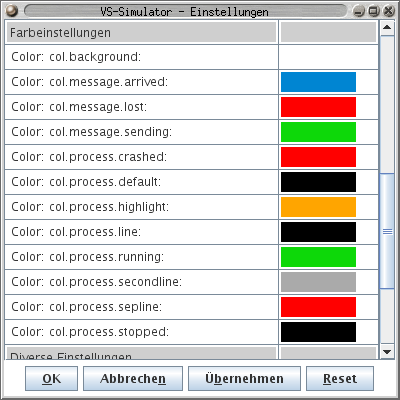
\includegraphics{images/ss-simulationseinstellungen-experten}}
	\caption{Weitere Simulationseinstellungen im Expertenmodus}
	\label{fig:SimulationseinstellungenExperten}
\end{figure}

Im selben Fenster lassen sich auch die Protokollvariablen editieren. Die Protokollvariablen werden jedoch sp\"{a}ter in der Protokollsektion beschrieben.

\subsection{Einstellungen im Expertenmodus}

\begin{table}
	\centering
	\fbox{
	\begin{tabular}{l|l}
		\textbf{Schl\"{u}ssel} & \textbf{Beschreibung}\\
		\hline 
			\texttt{col.background} & Die Hintergrundfarbe der Simulation\\
			\texttt{col.message.arrived} & Nachrichtenfarbe wenn sie ihr Ziel erreicht hat\\
			\texttt{col.message.lost} & Nachrichtenfarbe wenn sie verloren ging\\
			\texttt{col.message.sending} & Nachrichtenfarbe wenn sie noch unterwegs ist\\
			\textbf{\texttt{col.process.crashed}} & Prozessfarbe wenn er abgest\"{u}rzt ist\\
			\textbf{\texttt{col.process.default}} & Prozessfarbe wenn die Simulation aktuell nicht l\"{a}uft und \\
				& der Prozess aktuell nicht abgest\"{u}rzt ist \\
			\textbf{\texttt{col.process.highlight}} & Prozessfarbe wenn die Maus \"{u}ber seinem Balken liegt\\
			\texttt{col.process.line} & Farbe, in der die kleine ``Prozessfane'' an der auch die \\
				& lokale Prozesszeit angegeben wird, dargestellt wird\\
			\textbf{\texttt{col.process.running}} & Prozessfarbe wenn er nicht abgest\"{u}rzt ist und die\\
				& Simulation aktuell l\"{a}uft\\
			\texttt{col.process.secondline} & Farbe in der die Sekunden-Zeitgitter dargestellt werden \\
			\texttt{col.process.sepline} & Farbe der globalen Zeitachse\\
			\textbf{\texttt{col.process.stopped}} & Prozessfarbe wenn die Simulation pausiert wurde\\
	\end{tabular}
	}
	\caption{Farbeinstellungen}
	\label{tb:Farbeinstellungen}
\end{table}

Im Expertenmodus lassen sich zus\"{a}tzliche Variablen, wie beispielsweise diverse Farbwerte und Anzahl der Pixel verschiedener der GUI-Elemente, editieren. In Abbildung \ref{fig:SimulationseinstellungenExperten} sieht der Benutzer alle einstellbaren Farben. Die fett-gedruckten Schl\"{u}ssel in Tabelle \ref{tb:Farbeinstellungen} dienen nur als Standardwerte f\"{u}r neuzuerstellenen Prozesse und sind auch jeweils in den Prozesseinstellungen separat editierbar.

\section{Protokolle}

Im Folgenden werden alle bisher verf\"{u}gbaren Protokolle behandelt. Wie bereits beschrieben wird bei Protokollen zwischen Server- und Clientseite unterschieden. Server k\"{o}nnen auf Clientnachrichten, und Client auf Servernachrichten antworten. Jeder Prozess kann beliebig viele Protokolle sowohl Clientseitig als auch Serverseitig untest\"{u}tzen. Theoretisch ist es auch m\"{o}glich, dass ein Prozess f\"{u}r ein bestimmtes Protokoll gleichzeitig Server und Client ist. Der Benutzer kann auch weitere eigene Protokolle in der Programmiersprache Java mittels einer speziellen API (Application Programming Interface) erstellen. Wie eigene Protokolle erstellt werden k\"{o}nnen wird sp\"{a}ter behandelt. 

\subsection{Beispiel (Dummy) Protokoll}

Das Dummy-Protokoll dient lediglich als leeres Template f\"{u}r die Erstellung eigener Protokolle. Bei der Verwendung des Dummy-Protokolls werden bei Ereignissen lediglich Loggnachrichten ausgegeben. Es werden aber keine weiteren Aktionen ausgef\"{u}hrt.

\subsection{Das Ping-Pong Protokoll}

\begin{table}
	\centering
	\fbox{
	\begin{tabular}{c|c|l}
		\textbf{Zeit (ms)} & \textbf{PID} & \textbf{Ereignis} \\
		\hline 
		 	0 & 1 & Ping Pong Client aktivieren\\
		 	0 & 2 & Ping Pong Server aktivieren\\
		 	0 & 1 & Ping Pong Clientanfrage starten
	\end{tabular}
	}
	\caption{Programmierte Ping-Pong Ereignisse}
	\label{tb:PingPongTasks}
\end{table}


\begin{figure}[htbp]
	\centering
	\fbox{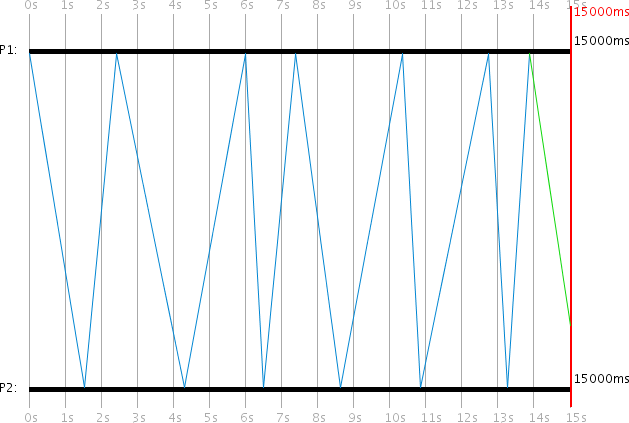
\includegraphics[width=10cm]{images/ss-protokoll-ping-pong}}
	\caption{Das Ping-Pong Protokoll}
	\label{fig:PingPongProto}
\end{figure}

Bei dem Ping-Pong Protokoll (Abbildung \ref{fig:PingPongProto}) werden zwischen zwei Prozessen, Client P1 und Server P2, st\"{a}ndig Nachrichten hin- und hergeschickt. Der Ping-Pong Client startet die erste Anfrage, worauf der Server dem Client antwortet. Auf diese Antwort wird vom Client wiederum geantwortet und so weiter. Jeder Nachricht wird ein Z\"{a}hler mitgeschickt, der bei jeder Station um eins inkrementiert- und jeweils im Loggfenster protokolliert wird. In der Simulation werden erst keine Antwortnachrichten mehr verschickt, wenn entweder eine Nachricht verloren geht, oder wenn die Simulationszeit das Ende erreicht hat. In Tabelle \ref{tb:PingPongTasks} sind alle f\"{u}r dieses Beispiel programmierten Ereignisse aufgef\"{u}hrt! Wichtig ist, dass Prozess 1 seinen Ping-Pong Client aktiviert, bevor er eine Ping-Pong Clientanfrage startet! Wenn die Eintrittszeiten f\"{u}r Aktivierung und das Starten der Anfrage identisch sind, so ordnet der Ereigniseditor diese Ereignisse automatisch in der richtigen Reihenfolge an. Wenn der Ping-Pong Client nicht aktiviert werden w\"{u}rde, dann k\"{o}nnte er auch keine Ping-Pong Anfrage starten. Dies gilt nat\"{u}rlich f\"{u}r alle anderen Protokolle analog. Anhand dieses Beispiels ist auch erkennbar, dass die noch nicht ausgelieferte Nachrichten noch g\"{u}n eingef\"{a}rbt ist. Alle ausgelieferten Nachrichten tragen bereits die Farbe Blau.

\begin{figure}[htbp]
	\centering
	\fbox{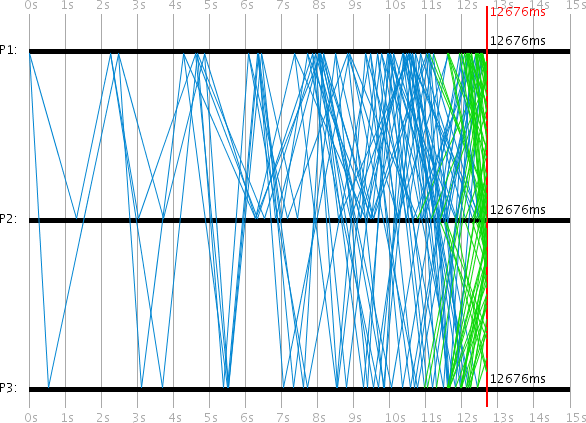
\includegraphics[width=10cm]{images/ss-protokoll-ping-pong-sturm}}
	\caption{Das Ping-Pong Protokoll (Sturm)}
	\label{fig:PingPongSturmProto}
\end{figure}

Werden die Ereignisse wie in Tabelle \ref{tb:PingPongSturmTasks} abge\"{a}ndert, so l\"{a}sst sich ein Ping-Pong Sturm realisieren. Dort wurde ein neuer Prozess 3 eingef\"{u}hrt, der als Ping-Pong Server fungiert. Als Ursache verdoppelt sich die Anzahl der kursierenden Nachrichten bei jedem Client-Server Roundtrip, da auf jede Clientnachricht stets 2 Serverantworten verschickt werden. In Abbildung \ref{fig:PingPongSturmProto} ist der resultierende Simulationsverlauf dargestellt.

\begin{table}
	\centering
	\fbox{
	\begin{tabular}{c|c|l}
		\textbf{Zeit (ms)} & \textbf{PID} & \textbf{Ereignis} \\
		\hline 
		 	0 & 1 & Ping Pong Client aktivieren\\
		 	0 & 2 & Ping Pong Server aktivieren\\
		 	0 & 3 & Ping Pong Server aktivieren\\
		 	0 & 1 & Ping Pong Clientanfrage starten
	\end{tabular}
	}
	\caption{Programmierte Ping-Pong Ereignisse (Sturm)}
	\label{tb:PingPongSturmTasks}
\end{table}

\subsection{Das Broadcast-Sturm Protokoll}

\begin{figure}[htbp]
	\centering
	\fbox{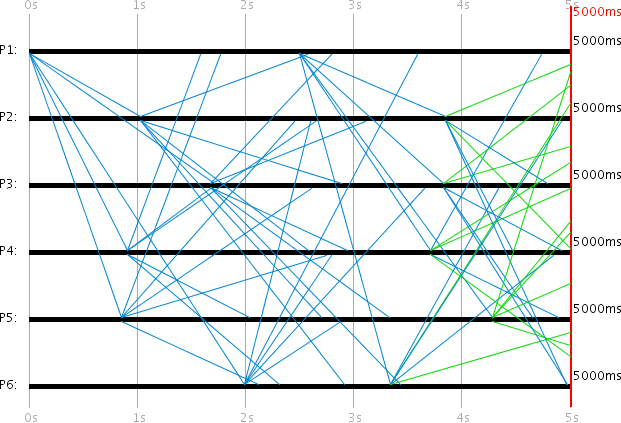
\includegraphics[width=10cm]{images/ss-protokoll-broadcast-sturm}}
	\caption{Das Broadcast-Sturm Protokoll}
	\label{fig:BroadcastSturmProto}
\end{figure}

Das Broadcast-Sturm Protokoll verh\"{a}lt sich \"{a}hnlich wie das Ping-Pong Protokoll. Der Unterschied besteht darin, dass sich das Protokoll anhand einer eindeutigen Broadcast-ID merkt, welche Nachrichten bereits verschickt wurden. Das Broadcast-Sturm Protokoll (Server- und Clientseitig) verschickt alle erhaltenen Nachrichten, sofern sie vom jeweiligen Prozess noch nicht schon einmal verschickt wurden, erneut. Somit l\"{a}sst sich, unter Verwendung mehrerer Prozesse (hier 6), wie auf Abbildung \ref{fig:BroadcastSturmProto}, ein Broadcast-Sturm erzeugen. P1 ist der Client und startet je eine Anfrage nach 0ms und 2500ms. Die Simulationsdauer betr\"{a}gt hier genau 5000ms. Da Client nur Servernachrichten und Server nur Clientnachrichten empfangen k\"{o}nnen, ist in dieser Simulation jeder Prozess, wie in Tabelle \ref{tb:BroadcastSturmTasks} angegeben, gleichzeitig Server und Client. 

\begin{table}
	\centering
	\fbox{
	\begin{tabular}{c|c|l}
		\textbf{Zeit (ms)} & \textbf{PID} & \textbf{Ereignis} \\
		\hline 
		 	0000 & 1 & Broadcaststurn Client aktivieren\\
		 	0000 & 2 & Broadcaststurn Client aktivieren\\
		 	0000 & 3 & Broadcaststurn Client aktivieren\\
		 	0000 & 4 & Broadcaststurn Client aktivieren\\
		 	0000 & 5 & Broadcaststurn Client aktivieren\\
		 	0000 & 6 & Broadcaststurn Client aktivieren\\
		 	0000 & 1 & Broadcaststurn Server aktivieren\\
		 	0000 & 2 & Broadcaststurn Server aktivieren\\
		 	0000 & 3 & Broadcaststurn Server aktivieren\\
		 	0000 & 4 & Broadcaststurn Server aktivieren\\
		 	0000 & 5 & Broadcaststurn Server aktivieren\\
		 	0000 & 6 & Broadcaststurn Server aktivieren\\
		 	0000 & 1 & Broadcaststurn Clientanfrage starten\\
		 	2500 & 1 & Broadcaststurn Clientanfrage starten
	\end{tabular}
	}
	\caption{Programmierte Broadcast-Sturm Ereignisse}
	\label{tb:BroadcastSturmTasks}
\end{table}

\subsection{Das Protokoll zur internen Synchronisierung in einem synchronen System}

Bisher haben wir uns nur mit Protokollen besch\"{a}ftigt, in denen die beteiligten Prozesse keine Uhrabweichung hatten. Das Protokoll zur internen Synchronisierung ist ein Protokoll zur Synchronisierung der lokalen Prozesszeit, welches beispielsweise angewandt werden kann, wenn eine Prozesszeit aufgrund einer Uhrabweichung falsch geht. Wenn der Client seine falsche lokale Zeit $t_c$ mit einem Server synchronisieren m\"{o}chte, so schickt er ihm eine Clientanfrage. Der Server schickt als Antwort seine eigene lokale Prozesszeit $t_s$ zur\"{u}ck, womit der Client seine neue und genauere Prozesszeit berechnen kann. Wie genau die neue Prozesszeit berechnet wird, wird im Folgenden beschrieben. 

\begin{table}
	\centering
	\fbox{
	\begin{tabular}{c|c|l}
		\textbf{Zeit (ms)} & \textbf{PID} & \textbf{Ereignis} \\
		\hline 
		 	00000 & 1 & Interne Sync. Client aktivieren \\
		 	00000 & 2 & Interne Sync. Server aktivieren\\
		 	00000 & 1 & Interne Sync. Clientanfrage starten\\
		 	05000 & 1 & Interne Sync. Clientanfrage starten\\
		 	10000 & 1 & Interne Sync. Clientanfrage starten\\
	\end{tabular}
	}
	\caption{Programmierte Ereignisse zur internen Synchronisierung}
	\label{tb:InterneSyncTasks}
\end{table}

Hier (Abbildung \ref{fig:TimeSyncProto}) stellt P1 den Client und P2 den Server dar. Da die \"{U}bertragungszeit $t_u$ einer Nachricht angenommen zwischen $t'_{min}$ und $t'_{max}$ liegt, setzt der Client P1 nach Empfang der Serverantwort seine lokale Prozesszeit auf $t_c := t_s + \frac{1}{2} (t'_{min} + t'_{max})$. Somit wurde die lokale Zeit von P1, bis auf einen Fehler $f$ mit $f < \frac{t'_{max} - t'_{min}}{2}$, synchronisiert. 

Der Clientprozess hat in der Abbildung \ref{fig:TimeSyncProto} als Uhrabweichung den Wert 0.1 und der Server hat als Uhrabweichung den Wert 0.0 konfiguriert. Der Client startet, wie in Tabelle \ref{tb:InterneSyncTasks} angegeben, nach 0ms, 5000ms und 10000ms seiner lokalen Prozesszeit jeweils eine Clientanfrage. In der Abbildung l\"{a}sst sich erkennen, dass die 2. und die 3. Anfrage nicht synchron zu der globalen Zeit (Sekunden-Gatter) gestartet werden. Dies ist auf die Uhrabweichung von P1 zur\"{u}ckzuf\"{u}hren. Nach Simulationsende ist die Zeit von P1 bis auf $15000ms - 15976ms = -976 ms$ synchronisiert.

\begin{figure}[htbp]
	\centering
	\fbox{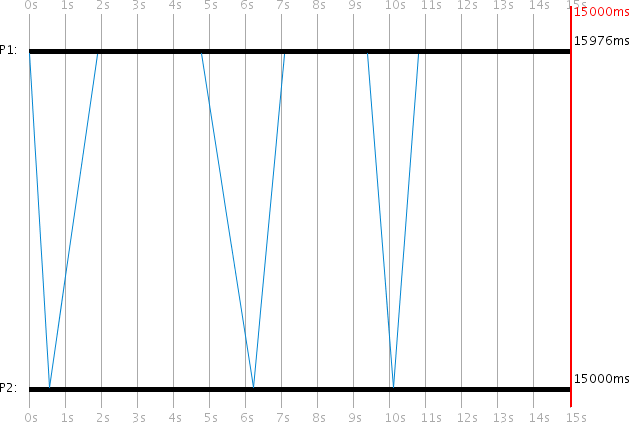
\includegraphics[width=10cm]{images/ss-protokoll-time-sync}}
	\caption{Das Protokoll zur internen Synchronisierung}
	\label{fig:TimeSyncProto}
\end{figure}

\subsubsection{Protokollvariablen}

Dieses Protokoll verwendet folgende zwei clientseitige Variablen, die in den Prozesseinstellungen unter dem Punkt ``Interne Sync. Client'' konfiguriert werden k\"{o}nnen. Serverseitig gibt es hier keine Variablen.

\begin{itemize}
	\item \textbf{Min. \"{U}bertragungszeit} \textit{(Long: 500)}: Gibt den Wert $t'_{min}$ in Millisekunden an
	\item \textbf{Max. \"{U}bertragungszeit} \textit{(Long: 2000)}: Gibt den Wert $t'_{max}$ in Millisekunden an
\end{itemize}

$t'_{min}$ und $t'_{max}$ sind die bei den Protokollberechnungen verwendeten Werte. Sie k\"{o}nnen sich allerdings von den tats\"{a}chlichen Nachrichten\"{u}bertragungszeiten $t_{min}$ und $t_{max}$ (siehe Sektion \"{u}ber Prozesseinstellungen) abweichen. Somit lassen sich auch Szenarien simulieren, in denen das Protokoll falsch konfiguriert wurde und die Zeitsynchronisation gr\"{o}ssere Ungenauigkeiten aufweisen kann.

\subsection{Christians Methode zur externen Synchronisierung}

\begin{figure}[htbp]
	\centering
	\fbox{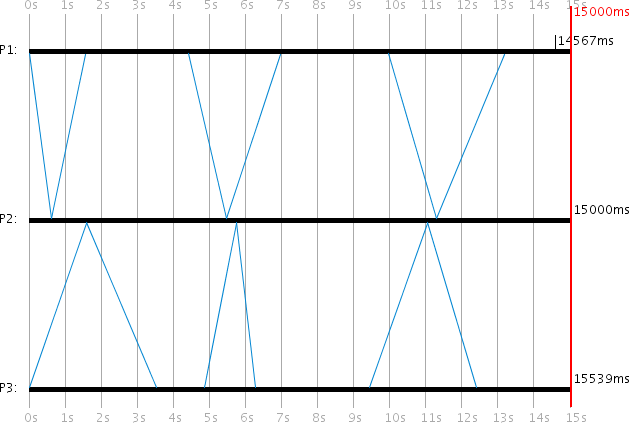
\includegraphics[width=10cm]{images/ss-protokoll-time-sync-2}}
	\caption{Interne Synchronisierung und Christians Methode im Vergleich}
	\label{fig:TimeSync2Proto}
\end{figure}

Ein weiteres Protokoll f\"{u}r die Synchronisierung von Uhrzeiten funktioniert nach der Christians Methode zur externen Synchronisierung. Die Christians Methode benutzt die RTT (Round Trip Zeit) $t_{rtt}$, um die \"{U}bertragungszeiten von einzelnen Nachrichten zu approximieren. 

Wenn der Client seine lokale Zeit $t_c$ bei einem Server synchronisieren m\"{o}chte, so verschickt er eine Anfrage, und misst dabei die RTT $t_{rtt}$ bis die Serverantwort eintrifft. Die Serverantwort beinhaltet die lokale Prozesszeit vom Server $t_s$ von dem Zeitpunkt, als der Server die Antwort verschickte. Der Client setzt dann seine lokale Zeit neu auf $t_c := t_s + \frac{1}{2} t_{rtt}$, und zwar mit einer Genauigkeit von $\pm(\frac{1}{2} t_{rtt} - u_{min}$) wenn $u_{min}$ eine Schranke f\"{u}r eine Nachrichten\"{u}bertragung mit $t_{rtt} < u_{min}$ ist (siehe \cite{Vorlesung}).

Im Prinzip sieht eine Christians-Simulation so aus wie in Abbildung \ref{fig:TimeSyncProto}, daher wird hier auf eine einfache Abbildung vom Christians-Protokoll verzichtet. Viel Interessanter ist der direkte Vergleich zwischen dem Protokoll zur internen Synchronisierung und der Christians Methode der externen Synchronisierung (Abbildung \ref{fig:TimeSync2Proto}). Hier stellt P1 den Client zur internen Synchronisierung und P3 den Client zur externen Synchronisierung dar. P2 fungiert f\"{u}r beide Protokolle gleichzeitig als Server. P1 und P3 starten jeweils zu den lokalen Prozesszeiten 0ms, 5000ms und 10000ms eine Clientanfrage (Tabelle \ref{tb:InterneSync2Tasks}). P1 und P3 haben als Uhrabweichung 0.1 eingestellt und die Simulationsdauer betr\"{a}gt insgesamt 15000ms.

Es ist zu ablesbar, dass P1 seine Zeit bis auf $15000ms - 14567ms = 433ms$ und P3 seine Zeit bis auf $15000ms - 15539ms = -539ms$ synchronisiert hat. In diesem Beispiel hat also das Protokoll zur internen Synchronisierung ein besseres Ergebnis geliefert. Dies ist allerdings nicht zwingend immer der Fall, da nach einer erneuten Ausf\"{u}hrung alle Nachrichten wieder eine neue zuf\"{a}llige \"{U}bertragungszeit haben werden, die auf das eine oder andere Protokoll schlechte oder gute Auswirkungen haben k\"{o}nnen.

\begin{table}
	\centering
	\fbox{
	\begin{tabular}{c|c|l}
		\textbf{Zeit (ms)} & \textbf{PID} & \textbf{Ereignis} \\
		\hline 
		 	00000 & 1 & Interne Sync. Client aktivieren \\
		 	00000 & 1 & Interne Sync. Clientanfrage starten\\
		 	00000 & 2 & Christians Server aktivieren\\
		 	00000 & 2 & Interne Sync. Server aktivieren\\
		 	00000 & 3 & Christians Client aktivieren \\
		 	00000 & 3 & Christians Clientanfrage starten\\
		 	05000 & 1 & Interne Sync. Clientanfrage starten\\
		 	05000 & 3 & Christians Clientanfrage starten\\
		 	10000 & 1 & Interne Sync. Clientanfrage starten\\
		 	10000 & 3 & Christians Clientanfrage starten\\
	\end{tabular}
	}
	\caption{Programmierte Ereignisse, Vergleich interne und externe Synchronisierung}
	\label{tb:InterneSync2Tasks}
\end{table}

\subsection{Der Berkeley Algorithmus zur internen Synchronisierung}

\begin{figure}[htbp]
	\centering
	\fbox{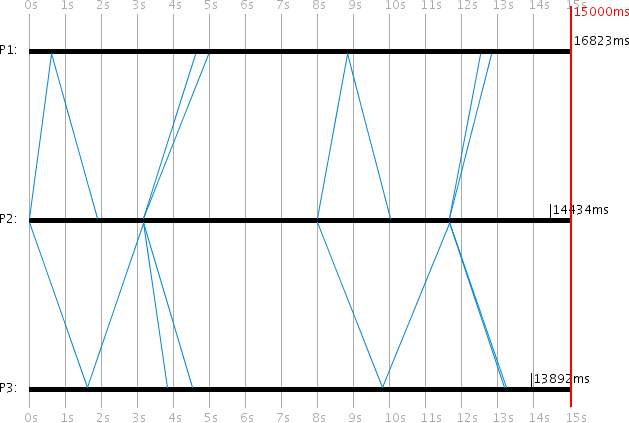
\includegraphics[width=10cm]{images/ss-protokoll-berkeley}}
	\caption{Der Berkeley Algorithmus zur internen Synchronisierung}
	\label{fig:BerkeleyProto}
\end{figure}

Der Berkeley Algorithmus zur internen Synchronisierung ist eine weitere M\"{o}glichkeit lokale Uhrzeiten abzugleichen. Dies ist das erste Protokoll, bei dem der Server die initiale Anfrage startet. Der Server stellt den Koordinator des Protokolls dar. Die Clients sind somit passiv und m\"{u}ssen warten, bis eine Serveranfrage eintritt. Hierbei muss der Server wissen, welche Clientprozesse an dem Protokoll teilnehmen, was sich in den Prozesseinstellungen des Servers einstellen l\"{a}sst.

\begin{table}
	\centering
	\fbox{
	\begin{tabular}{c|c|l}
		\textbf{Zeit (ms)} & \textbf{PID} & \textbf{Ereignis} \\
		\hline 
		 	0000 & 1 & Berkeley Client aktivieren \\
		 	0000 & 2 & Berkeley Server aktivieren \\
		 	0000 & 3 & Berkeley Client aktivieren \\
		 	0000 & 2 & Berkeley Serveranfrage starten\\
		 	7500 & 2 & Berkeley Serveranfrage starten\\
	\end{tabular}
	}
	\caption{Programmierte Ereignisse zum Berkeley Algorithmus}
	\label{tb:BerkeleyTasks}
\end{table}

Wenn der Server seine eigene lokale Zeit $t_s$ und auch die lokalen Prozesszeiten $t_i$ der Clients ($i = 1, ..., n$) synchronisieren m\"{o}chte, so verschickt er eine Serveranfrage. $n$ sei hierbei die Anzahl beteiligter Clients. Die Clients senden dann ihre lokalen Prozesszeiten in einer Nachricht zur\"{u}ck zum Server. Der Server hat dabei die RTTs $r_i$ bis zur Ankunft aller Clientantworten gemessen. Nachdem alle Antworten vorliegen, setzt er zun\"{a}chst seine eigene Zeit $t_s$ auf den Mittelwert seiner eigener Zeit sowie aller Prozesszeiten. Die \"{U}bertragungszeit einer Clientantwort wird auf die h\"{a}lfte der RTT gesch\"{a}tzt und wird in der Berechnung ber\"{u}cksichtigt:

\begin{equation*}
	t_{avg} :=
	\frac{1}{n+1} ( t_s +
		\sum_{\substack{
			i=1\\
		}}^n
		\frac{r_i}{2} + t_i
	)
\end{equation*}
\begin{equation*}
	t_s := t_{avg}
\end{equation*}

Anschlie�end berechnet der Server f\"{u}r jeden Client einen Korrekturwert $k_i := t_{avg} - t_i$, den er jeweils in einer separaten Nachricht zur\"{u}ckschickt. Die Clients setzten dann jeweils die lokale Prozesszeit auf $t'_i := t'_i + k_i$. Hierbei stellt $t'_i$ die derzeit aktuelle Prozesszeit des jeweiligen Clients dar. Denn bis zum Eintreffen des Korrekturwertes ist inzwischen wieder Zeit verstrichen.

In den Beispiel in Abbildung \ref{fig:BerkeleyProto} gibt es 2 Clientprozesse P1 und P3 sowie den Serverprozess P2. Der Server startet nach jeweils 0ms und 7500ms eine Synchronisationsanfrage (Tabelle \ref{tb:BerkeleyTasks}). In der Abbildung ist zu erkennen, dass der Server stets 2 Korrekturwerte verschickt, die jeweils P1 und P2 erreichen. Es werden hier also pro Synchronisierungsvorgang 4 Korrekturwerte ausgeliefert. Eine Korrekturnachricht enth\"{a}lt neben dem Korrekturwert $k_i$ auch die PID des Prozesses, f\"{u}r den die Nachricht bestimmt ist. Ein Client verarbeiten so nur die f\"{u}r ihn bestimmten Korrekturwerte, indem das Protokoll die PID vorher \"{u}berpr\"{u}ft. 

\subsubsection{Protokollvariablen}

Dieses Protokoll verwendet folgende serverseitige Variable, die in den Prozesseinstellungen unter dem Punkt ``Berkeley Server'' konfiguriert werden kann. Clientseitig gibt es hier keine Variablen.

\begin{itemize}
	\item \textbf{PIDs beteiliger Prozesse} \textit{(Integer[]: [1,3])}: Dieser Vektor aus Integerwerten beinhaltet alle PIDs der Berkeley Clientprozesse, mit denen der Berkeley Server synchronisieren soll. Wenn hier eine PID angegeben wird, die gar nicht existiert oder nicht das Berkeley Protokoll clientseitig unterst\"{u}tz, funktioniert das Protokoll nicht. Dann wird ewig auf eine fehlende Clientantwort gewartet.
\end{itemize}

\subsection{Das Ein-Phasen Commit Protokoll}

\begin{figure}[htbp]
	\centering
	\fbox{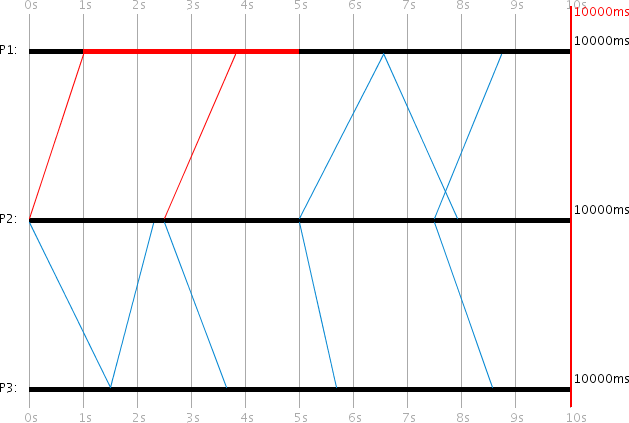
\includegraphics[width=10cm]{images/ss-protokoll-one-phase-commit}}
	\caption{Das Ein-Phasen Commit Protokoll}
	\label{fig:OnePhaseCommitProto}
\end{figure}

Das Ein-Phasen Commit Protokoll ist daf\"{u}r da, beliebig vielen Clients zu einer Festschreibung zu bewegen. Im realen Leben k\"{o}nnte dies beispielsweise das Erstellen oder L\"{o}schen einer Datei sein, von der auf jedem Client eine lokale Kopie existiert. Der Server ist der Koordinator und auch derjenige, der einen Festschreibewunsch initiiert. Hierbei verschickt der Server periodisch so oft den Festschreibewunsch, bis er von jedem Client eine Best\"{a}tigung erhalten hat. Der Server muss dabei die PIDs aller beteiligten Clientprozesse sowie einen Wecker f\"{u}r erneutes Versenden des Festschreibewunsches eingestellt bekommen. 

Die programmierten Ereignisse des Beispiels in Abbildung \ref{fig:OnePhaseCommitProto} sind in Tabelle \ref{tb:OnePhaseCommitTasks} aufgelistet. P1 und P3 simulieren jeweils einen Client und P2 den Server. Damit die Simulation mehrere Festschreibew\"{u}nsche verschickt, st\"{u}rzt in der Simulation P1 nach 1000ms ab und nach 5000ms steht er wieder zur Verf\"{u}gung. Die ersten beide Festschreibew\"{u}nsche erreichen dadurch P1 nicht und erst der dritte Versuch verl\"{a}uft erfolgreich. Bevor die Best\"{a}tigung von P1 bei P2 eintrifft, l\"{a}uft jedoch der Wecker erneut ab, so dass ein weiterer Festschreibewunsch versendet wird. Da P1 und P3 jeweils schon eine Best\"{a}tigung verschickt haben, wird dieser Wunsch ignoriert.

\begin{table}
	\centering
	\fbox{
	\begin{tabular}{c|c|l}
		\textbf{Zeit (ms)} & \textbf{PID} & \textbf{Ereignis} \\
		\hline 
		 	0000 & 1 & 1-Phasen Commit Client aktivieren\\
		 	0000 & 2 & 1-Phasen Commit Server aktivieren\\
		 	0000 & 3 & 1-Phasen Commit Client aktivieren\\
		 	0000 & 2 & 1-Phasen Commit Serveranfrage starten\\
		 	1000 & 1 & Prozessabsturz\\
		 	5000 & 1 & Prozesswiederbelebung
	\end{tabular}
	}
	\caption{Programmierte Ein-Phasen Commit Ereignisse}
	\label{tb:OnePhaseCommitTasks}
\end{table}

\subsubsection{Protokollvariablen}

Dieses Protokoll verwendet folgende serverseitige Variablen, die in den Prozesseinstellungen unter dem Punkt ``1-Phasen Commit Server'' konfiguriert werden kann. Clientseitig gibt es hier keine Variablen.

\begin{itemize}
	\item \textbf{Zeit bis erneute Anfrage} \textit{(Long: 2500)}: Gibt die Anzahl von Millisekunden an, die gewartet werden sollen, bis der Festschreibewunsch erneut verschickt wird.
	\item \textbf{PIDs beteiliger Prozesse} \textit{(Integer[]: [1,3])}: Dieser Vektor aus Integerwerten beinhaltet alle PIDs der Clientprozesse, die festschreiben sollen. 
\end{itemize}

\subsection{Das Zwei-Phasen Commit Protokoll}

\begin{figure}[htbp]
	\centering
	\fbox{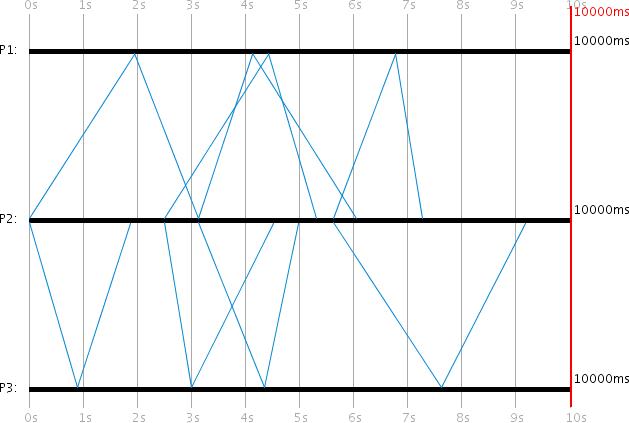
\includegraphics[width=10cm]{images/ss-protokoll-two-phase-commit}}
	\caption{Das Zwei-Phasen Commit Protokoll}
	\label{fig:TwoPhaseCommitProto}
\end{figure}

Das Zwei-Phasen Commit Protokoll ist eine Erweiterung des Ein-Phasen Commit Protokolls. Der Server startet zun\"{a}chst eine Anfrage an alle beteiligten Clients, ob festgeschrieben werden soll. Jeder Client antwortet dann mit true oder false. Der Server fragt so oft periodisch nach, bis ein Ergebnis aller Clients vorliegt. Nach Erhalt aller Abstimmungen \"{u}berpr\"{u}ft der Server, ob alle mit true abgestimmt haben. F\"{u}r den Fall dass mindestens ein Client mit false abgestimmt hat, wird der Festschreibevorgang abgebrochen und als globales Abstimmungsergebnis false verschickt. Wenn alle jedoch mit true abstimmten, soll festgeschrieben werden. Dabei wird das globale Abstimmungsergebnis true verschickt. Das globale Abstimmungsergebnis wird periodisch so oft erneut verschickt, bis von jedem Client eine Best\"{a}tigung des Erhalts vorliegt.

\begin{table}
	\centering
	\fbox{
	\begin{tabular}{c|c|l}
		\textbf{Zeit (ms)} & \textbf{PID} & \textbf{Ereignis} \\
		\hline 
		 	0000 & 1 & 2-Phasen Commit Client aktivieren\\
		 	0000 & 2 & 2-Phasen Commit Server aktivieren\\
		 	0000 & 3 & 2-Phasen Commit Client aktivieren\\
		 	0000 & 2 & 2-Phasen Commit Serveranfrage starten
	\end{tabular}
	}
	\caption{Programmierte Zwei-Phasen Commit Ereignisse}
	\label{tb:TwoPhaseCommitTasks}
\end{table}

In dem Beispiel (Abbildung \ref{fig:TwoPhaseCommitProto}) sind P1 und P3 Clients und P2 der Server. Der Server verschickt nach 0ms seine initiale Anfrage (Tabelle \ref{tb:TwoPhaseCommitTasks}). Da diese Simulation recht un\"{u}bersichtlich ist, liegen In den Tabellen \ref{tb:TwoPhaseCommitLoggs} und \ref{tb:TwoPhaseCommitLoggs2} Ausz\"{u}ge dem Loggfenster vor. Hier stimmen P1 und P3 jeweils mit true, d.h. es soll festgeschrieben werden, ab. Auf die Lamport- und Vektorzeitstempel sowie die lokalen Prozesszeiten wurde in der Darstellung wegen Irrelevanz verzichtet. Da keine Uhrabweichungen konfiguriert wurden, sind die lokalen Prozesszeiten stets gleich der globalen Zeit. Anhand der Nachrichten IDs lassen sich dort die einzelnen Sendungen zuordnen. In den Loggs wird auch st\"{a}ndig der Inhalt der verschickten Nachricht sowie die dazugeh\"{o}rigen Datentypen aufgef\"{u}hrt.

\begin{table}
	\centering
	\fbox{
	\begin{tabular}{c|c|l}
		\textbf{Zeit (ms)} & \textbf{PID} & \textbf{Loggnachricht} \\
			\hline
000000 & & Simulation gestartet\\
\hline
000000 & 1 & 2-Phasen Commit Client aktiviert\\
\hline
000000 & 2 & 2-Phasen Commit Server aktiviert\\
\hline
000000 & 2 & Nachricht versendet; ID: 94; Protokoll: 2-Phasen Commit\\
	& & Boolean: wantVote=true\\
\hline
000000 & 3 & 2-Phasen Commit Client aktiviert\\
\hline
000905 & 3 & Nachricht erhalten; ID: 94; Protokoll: 2-Phasen Commit\\
\hline
000905 & 3 & Nachricht versendet; ID: 95; Protokoll: 2-Phasen Commit\\
	& & Integer: pid=3; Boolean: isVote=true; vote=true\\
\hline
000905 & 3 & Abstimmung true versendet\\
\hline
001880 & 2 & Nachricht erhalten; ID: 95; Protokoll: 2-Phasen Commit\\
\hline
001880 & 2 & Abstimmung von Prozess 3 erhalten! Ergebnis: true\\
\hline
001947 & 1 & Nachricht erhalten; ID: 94; Protokoll: 2-Phasen Commit\\
\hline
001947 & 1 & Nachricht versendet; ID: 96; Protokoll: 2-Phasen Commit\\
	& & Integer: pid=1; Boolean: isVote=true; vote=true\\
\hline
001947 & 1 & Abstimmung true versendet\\
\hline
002500 & 2 & Nachricht versendet; ID: 97; Protokoll: 2-Phasen Commit\\
	& & Boolean: wantVote=true\\
\hline
003006 & 3 & Nachricht erhalten; ID: 97; Protokoll: 2-Phasen Commit\\
\hline
003006 & 3 & Nachricht versendet; ID: 98; Protokoll: 2-Phasen Commit\\
	& & Integer: pid=3; Boolean: isVote=true; vote=true\\
\hline
003006 & 3 & Abstimmung true versendet\\
\hline
003137 & 2 & Nachricht erhalten; ID: 96; Protokoll: 2-Phasen Commit\\
\hline
003137 & 2 & Abstimmung von Prozess 1 erhalten! Ergebnis: true\\
\hline
003137 & 2 & Abstimmungen von allen beteiligten Prozessen erhalten!\\
	& & Globales Ergebnis: true\\
\hline
003137 & 2 & Nachricht versendet; ID: 99; Protokoll: 2-Phasen Commit\\
	& & Boolean: isVoteResult=true; voteResult=true\\
\hline
004124 & 1 & Nachricht erhalten; ID: 99; Protokoll: 2-Phasen Commit\\
\hline
004124 & 1 & Globales Abstimmungsergebnis erhalten. Ergebnis: true\\
\hline
004124 & 1 & Nachricht versendet; ID: 100; Protokoll: 2-Phasen Commit\\
	& & Integer: pid=1; Boolean: isAck=true\\
\hline
004354 & 3 & Nachricht erhalten; ID: 99; Protokoll: 2-Phasen Commit\\
\hline
004354 & 3 & Globales Abstimmungsergebnis erhalten. Ergebnis: true\\
\hline
004354 & 3 & Nachricht versendet; ID: 101; Protokoll: 2-Phasen Commit\\
	& & Integer: pid=3; Boolean: isAck=true\\
\hline
004434 & 1 & Nachricht erhalten; ID: 97; Protokoll: 2-Phasen Commit\\
\hline
004434 & 1 & Nachricht versendet; ID: 102; Protokoll: 2-Phasen Commit\\
	& & Integer: pid=1; Boolean: isVote=true; vote=true\\
	\end{tabular}
	}
	\caption{Auszug aus der Loggausgabe des Zwei-Phasen Commit Beispiels}
	\label{tb:TwoPhaseCommitLoggs}
\end{table}

\begin{table}
	\centering
	\fbox{
	\begin{tabular}{c|c|l}
		\textbf{Zeit (ms)} & \textbf{PID} & \textbf{Loggnachricht} \\
			\hline
004434 & 1 & Abstimmung true versendet\\
\hline
004527 & 2 & Nachricht erhalten; ID: 98; Protokoll: 2-Phasen Commit\\
\hline
004975 & 2 & Nachricht erhalten; ID: 101; Protokoll: 2-Phasen Commit\\
\hline
005311 & 2 & Nachricht erhalten; ID: 102; Protokoll: 2-Phasen Commit\\
\hline
005637 & 2 & Nachricht versendet; ID: 103; Protokoll: 2-Phasen Commit\\
	& & Boolean: isVoteResult=true; voteResult=true\\
\hline
006051 & 2 & Nachricht erhalten; ID: 100; Protokoll: 2-Phasen Commit\\
\hline
006051 & 2 & Alle Teilnehmer haben die Abstimmung erhalten\\
\hline
006766 & 1 & Nachricht erhalten; ID: 103; Protokoll: 2-Phasen Commit\\
\hline
006766 & 1 & Globales Abstimmungsergebnis erhalten. Ergebnis: true\\
\hline
006766 & 1 & Nachricht versendet; ID: 104; Protokoll: 2-Phasen Commit\\
	& & Integer: pid=1; Boolean: isAck=true\\
\hline
007279 & 2 & Nachricht erhalten; ID: 104; Protokoll: 2-Phasen Commit\\
\hline
007618 & 3 & Nachricht erhalten; ID: 103; Protokoll: 2-Phasen Commit\\
\hline
007618 & 3 & Globales Abstimmungsergebnis erhalten. Ergebnis: true\\
\hline
007618 & 3 & Nachricht versendet; ID: 105; Protokoll: 2-Phasen Commit\\
	& & Integer: pid=3; Boolean: isAck=true\\
\hline
009170 & 2 & Nachricht erhalten; ID: 105; Protokoll: 2-Phasen Commit\\
\hline
010000 & & Simulation beendet
	\end{tabular}
	}
	\caption{Auszug aus der Loggausgabe des Zwei-Phasen Commit Beispiels (2)}
	\label{tb:TwoPhaseCommitLoggs2}
\end{table}

\subsubsection{Protokollvariablen}

Dieses Protokoll verwendet folgende serverseitige Variablen, die in den Prozesseinstellungen unter dem Punkt ``2-Phasen Commit Server'' konfiguriert werden k\"{o}nnen:

\begin{itemize}
	\item \textbf{Zeit bis erneute Anfrage} \textit{(Long: 2500)}: Gibt die Anzahl von Millisekunden an, die gewartet werden sollen, bis der Festschreibewunsch erneut verschickt wird.
	\item \textbf{PIDs beteiliger Prozesse} \textit{(Integer[]: [1,3])}: Dieser Vektor aus Integerwerten beinhaltet alle PIDs der Clientprozesse, die \"{u}ber eine Festschreibung abstimmen, und anschlie�end gegebenenfalls festschreiben sollen. 
\end{itemize}

Und folgende Clientvariable kann unter den Prozesseinstellungen unter dem Punkt ``2-Phasen Commit Client'' konfiguriert werden:

\begin{itemize}
	\item \textbf{Festschreibwahrscheinlichkeit} \textit{(Integer: 50)}: Gibt die Wahrscheinlichkeit in Prozent an, die der Client mit true, also f\"{u}r das Festschreiben, abstimmt.
\end{itemize}

\subsection{Der ungen\"{u}gende (Basic) Multicast}

\begin{figure}[htbp]
	\centering
	\fbox{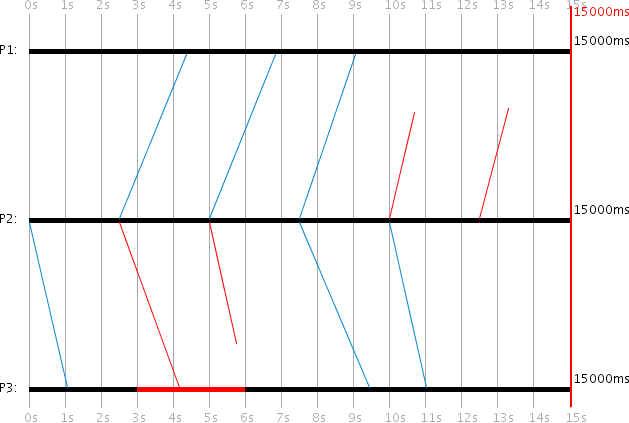
\includegraphics[width=10cm]{images/ss-protokoll-basic-multicast}}
	\caption{Das Basic-Multicast Protokoll}
	\label{fig:BasicMulticastProto}
\end{figure}

Das Basic-Multicast Protokoll ist sehr einfach aufgebaut. In dem Beispiel auf Abbildung \ref{fig:BasicMulticastProto} sind P1 und P3 Server und P2 der Client. Bei diesem Protokoll startet der Client immer die Anfrage, was bei diesem Protokoll eine einfache Multicast-Nachricht ist, die jeder Server empfangen kann. Wie in Tabelle \ref{tb:BasicMulticastTasks} aufgef\"{u}hrt verschickt P2 alle 2500ms jeweils eine Multicast-Nachricht, die alle voneinander v\"{o}llig unabh\"{a}ngig sind. P1 kann jedoch erst nach 2500ms Multicast-Nachrichten empfangen, da er vorher das Protokoll nicht unterst\"{u}tzt w\"{a}hrend P3 von 3000ms bis 6000ms abgest\"{u}rzt ist und auch keine Nachrichten empfangen kann. Da die Einstellung ``Nur relevante Nachrichten anzeigen'' aktiviert ist, wird die erste Multicast-Nachricht von P2 an P1 nicht dargestellt. Bei jedem Prozess wurde die Nachrichtenverlustwahrscheinlichkeit auf 30 Prozent gesetzt, worauf alle in dieser Simulation verschickten Nachrichten mit einer Wahrscheinlichkeit von 30 Prozent ausfallen. Hier ging die 3. Multicast-Nachricht auf den Weg zu P3- und die 5. sowie 6. Nachricht auf den Weg zu P1 verloren.

\begin{table}
	\centering
	\fbox{
	\begin{tabular}{c|c|l}
		\textbf{Zeit (ms)} & \textbf{PID} & \textbf{Ereignis} \\
		\hline 
		 	00000 & 2 & Basic Multicast Client aktivieren\\
		 	00000 & 3 & Basic Multicast Server aktivieren\\
		 	00000 & 2 & Basic Multicast Clientanfrage starten\\
		 	02500 & 1 & Basic Multicast Server aktivieren\\
		 	02500 & 2 & Basic Multicast Clientanfrage starten\\
		 	03000 & 3 & Prozessabsturz\\
		 	05000 & 2 & Basic Multicast Clientanfrage starten\\
		 	06000 & 3 & Prozesswiederbelebung\\
		 	07500 & 2 & Basic Multicast Clientanfrage starten\\
		 	10000 & 2 & Basic Multicast Clientanfrage starten\\
		 	12500 & 2 & Basic Multicast Clientanfrage starten
	\end{tabular}
	}
	\caption{Programmierte Basic-Multicast Ereignisse}
	\label{tb:BasicMulticastTasks}
\end{table}

\subsection{Der zuverl\"{a}ssige (Reliable) Multicast}

\begin{figure}[htbp]
	\centering
	\fbox{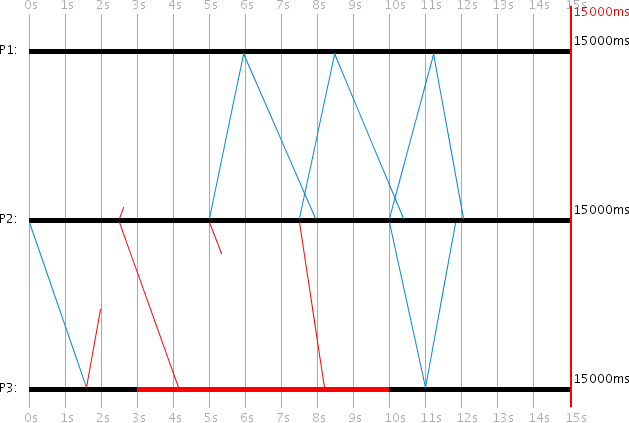
\includegraphics[width=10cm]{images/ss-protokoll-reliable-multicast}}
	\caption{Das Reliable-Multicast Protokoll}
	\label{fig:ReliableMulticastProto}
\end{figure}

Bei dem  zuverl\"{a}ssigen (Reliable) Multicast verschickt der Client so oft periodisch seine Multicast-Nachricht, bis er von allen beteiligten Servern eine Best\"{a}tigung erhalten hat. Nach jedem erneuten Versuch vergisst der Client, von welchen Servern er bereits eine Best\"{a}tigung erhalten hat, womit jeder erneuter Versuch von allen Teilnehmern aufs Neue best\"{a}tigt werden muss. In dem Beispiel (Abbildung \ref{fig:ReliableMulticastProto}, Tabelle \ref{tb:ReliableMulticastTasks}, sowie den Loggs in den Tabellen \ref{tb:ReliableMulticastLoggs} und \ref{tb:ReliableMulticastLoggs2}) ist P2 der Multicast-verschickende Client, w\"{a}hrend P1 und P3 die Server sind. Bei 0ms initiiert der Client seine Multicast-Nachricht. Die Nachrichtenverlustwahrscheinlichkeiten sind \"{u}berall auf 30 Prozent eingestellt.

In diesem Beispiel ben\"{o}tigt der Client bis zur korrekten Auslieferung eines zuverl\"{a}ssigen Multicasts genau 5 Versuche:

\begin{enumerate}
	\setlength{\itemsep}{-2mm}
	\item Versuch: 
		\begin{itemize}
			\setlength{\itemsep}{-2.5mm}
			\item P1 unterst\"{u}tzt das Reliable-Multicast Protokoll noch nicht, und kann somit weder Multicast-Nachricht erhalten noch eine Best\"{a}tigung verschicken.
			\item P3 empf\"{a}ngt die Multicast-Nachricht, jedoch geht seine Best\"{a}tigungsnachricht verloren.
		\end{itemize}
	\item Versuch: 
		\begin{itemize}
			\setlength{\itemsep}{-2.5mm}
			\item P1: Die Multicast-Nachricht geht unterwegs zu P1 verloren.
			\item P3: Die Multicast-Nachricht erreicht P3, aber P3 ist abgest\"{u}rzt und kann somit keine Nachricht verarbeiten.
		\end{itemize}
	\item Versuch: 
		\begin{itemize}
			\setlength{\itemsep}{-2.5mm}
			\item P1 empf\"{a}ngt die Multicast-Nachricht und seine Best\"{a}tigung kommt wie geplant bei P2 an. 
			\item P3: Die Multicast-Nachricht geht unterwegs zu P3 verloren.
		\end{itemize}
	\item Versuch: 
		\begin{itemize}
			\setlength{\itemsep}{-2.5mm}
			\item P1 empf\"{a}ngt die Multicast-Nachricht und seine Best\"{a}tigung kommt wie geplant bei P2 an. 
			\item P3: Die Multicast-Nachricht erreicht P3, aber P3 ist abgest\"{u}rzt und kann somit keine Nachricht verarbeiten.
		\end{itemize}
	\item Versuch: 
		\begin{itemize}
			\item P1 empf\"{a}ngt die Multicast-Nachricht und seine Best\"{a}tigung kommt wie geplant bei P2 an. 
			\setlength{\itemsep}{-2.5mm}
			\item P3 empf\"{a}ngt die Multicast-Nachricht und seine Best\"{a}tigung kommt wie geplant bei P2 an. 
		\end{itemize}
\end{enumerate}

\begin{table}
	\centering
	\fbox{
	\begin{tabular}{c|c|l}
		\textbf{Zeit (ms)} & \textbf{PID} & \textbf{Ereignis} \\
		\hline 
		 	00000 & 3 & Reliable Multicast Server aktivieren\\
		 	00000 & 2 & Reliable Multicast Client aktivieren\\
		 	00000 & 2 & Reliable Multicast Clientanfrage starten\\
		 	02500 & 1 & Reliable Multicast Server aktivieren\\
		 	03000 & 3 & Prozessabsturz\\
		 	10000 & 3 & Prozesswiederbelebung\\
	\end{tabular}
	}
	\caption{Programmierte Reliable-Multicast Ereignisse}
	\label{tb:ReliableMulticastTasks}
\end{table}

\begin{table}
	\centering
	\fbox{
	\begin{tabular}{c|c|l}
		\textbf{Zeit (ms)} & \textbf{PID} & \textbf{Loggnachricht} \\
			\hline
000000 & & Simulation gestartet\\
\hline
000000 & 2 & Reliable Multicast Client aktiviert\\
\hline
000000 & 2 & Nachricht versendet; ID: 280; Protokoll: Reliable Multicast;\\
	   & & Boolean: isMulticast=true\\
\hline
000000 & 3 & Reliable Multicast Server aktiviert\\
\hline
001590 & 3 & Nachricht erhalten; ID: 280; Protokoll: Reliable Multicast\\
\hline
001590 & 3 & Nachricht versendet; ID: 281; Protokoll: Reliable Multicast\\
	   & & Integer: pid=3; Boolean: isAck=true\\
\hline
001590 & 3 & ACK versendet\\
\hline
002500 & 1 & Reliable Multicast Server aktiviert\\
\hline
002500 & 2 & Nachricht versendet; ID: 282; Protokoll: Reliable Multicast\\
	   & & Boolean: isMulticast=true\\
\hline
003000 & 3 & Abgest�rzt\\
\hline
005000 & 2 & Nachricht versendet; ID: 283; Protokoll: Reliable Multicast\\
	   & & Boolean: isMulticast=true\\
\hline
005952 & 1 & Nachricht erhalten; ID: 283; Protokoll: Reliable Multicast\\
\hline
005952 & 1 & Nachricht versendet; ID: 284; Protokoll: Reliable Multicast\\
	   & & Integer: pid=1; Boolean: isAck=true\\
\hline
005952 & 1 & ACK versendet\\
\hline
007500 & 2 & Nachricht versendet; ID: 285; Protokoll: Reliable Multicast\\
	   & & Boolean: isMulticast=true\\
\hline
007937 & 2 & Nachricht erhalten; ID: 284; Protokoll: Reliable Multicast\\
\hline
007937 & 2 & ACK von Prozess 1 erhalten!\\
\hline
008469 & 1 & Nachricht erhalten; ID: 285; Protokoll: Reliable Multicast\\
\hline
008469 & 1 & Nachricht versendet; ID: 286; Protokoll: Reliable Multicast\\
	   & & Integer: pid=1; Boolean: isAck=true\\
\hline
008469 & 1 & ACK erneut versendet\\
\hline
010000 & 2 & Nachricht versendet; ID: 287; Protokoll: Reliable Multicast\\
	   & & Boolean: isMulticast=true\\
\hline
010000 & 3 & Wiederbelebt\\
\hline
010395 & 2 & Nachricht erhalten; ID: 286; Protokoll: Reliable Multicast\\
\hline
010995 & 3 & Nachricht erhalten; ID: 287; Protokoll: Reliable Multicast\\
\hline
010995 & 3 & Nachricht versendet; ID: 288; Protokoll: Reliable Multicast\\
	   & & Integer: pid=3; Boolean: isAck=true\\
\hline
010995 & 3 & ACK erneut versendet\\
\hline
011213 & 1 & Nachricht erhalten; ID: 287; Protokoll: Reliable Multicast\\
\hline
011213 & 1 & Nachricht versendet; ID: 289; Protokoll: Reliable Multicast\\
	   & & Integer: pid=1; Boolean: isAck=true\\
	\end{tabular}
	}
	\caption{Auszug aus der Loggausgabe des Reliable-Multicast Beispiels}
	\label{tb:ReliableMulticastLoggs}
\end{table}

\begin{table}
	\centering
	\fbox{
	\begin{tabular}{c|c|l}
		\textbf{Zeit (ms)} & \textbf{PID} & \textbf{Loggnachricht} \\
			\hline
011213 & 1 & ACK erneut versendet\\
\hline
011813 & 2 &  Nachricht erhalten; ID: 288; Protokoll: Reliable Multicast\\
\hline
011813 & 2 &  ACK von Prozess 3 erhalten!\\
\hline
011813 & 2 &  ACKs von allen beteiligten Prozessen erhalten!\\
\hline
012047 & 2 &  Nachricht erhalten; ID: 289; Protokoll: Reliable Multicast\\
\hline
015000 & & Simulation beendet\\
	\end{tabular}
	}
	\caption{Auszug aus der Loggausgabe des Reliable-Multicast Beispiels (2)}
	\label{tb:ReliableMulticastLoggs2}
\end{table}

\subsubsection{Protokollvariablen}

Dieses Protokoll verwendet folgende serverseitige Variablen, die in den Prozesseinstellungen unter dem Punkt ``Reliable Multicast Server'' konfiguriert werden k\"{o}nnen:

\begin{itemize}
	\item \textbf{Zeit bis erneute Anfrage} \textit{(Long: 2500)}: Gibt die Anzahl von Millisekunden an, die gewartet werden sollen, bis der Muticast erneut verschickt wird.
	\item \textbf{PIDs beteiliger Prozesse} \textit{(Integer[]: [1,3])}: Dieser Vektor aus Integerwerten beinhaltet alle PIDs der Serverprozesse, die die Multicast-Nachricht erhalten sollen.
\end{itemize}

\section{Weitere Beispiele}

Bisher wurden alle verf\"{u}gbaren Protokolle mit jeweils mindestens einem Beispiel aufgef\"{u}hrt. Mit dem Simulator lassen sich allerdings viel mehr Szenarien simulieren. Daher soll hier auf weitere Anwendungsbeispiele eingegangen werden.

\subsection{Vektor- und Lamportzeitstempel}

\begin{figure}[htbp]
	\centering
	\fbox{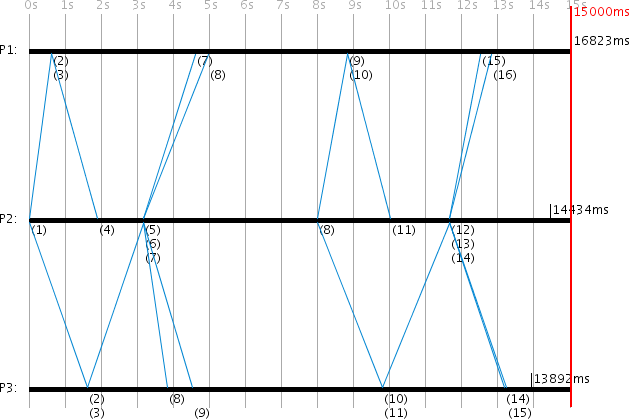
\includegraphics[width=10cm]{images/ss-protokoll-berkeley-lamport}}
	\caption{Lamportzeitstempel}
	\label{fig:Lamportzeit}
\end{figure}

Die Vektor- und Lamportzeitstempel lassen sich sehr gut am bereits behandelten Beispiel zum Berkeley-Protokoll demonstrieren. Nach Aktivierung der Lamportzeit-Checkbox erscheinen bei jedem Ereignis die zum jeweiligen Prozess geh\"{o}rigen Lamportzeitstempel (Abbildung \ref{fig:Lamportzeit}). Jeder Prozess besitzt einen eigenen Lamportzeitstempel, der bei jedem Versenden oder Erhalten einer Nachricht inkrementiert wird. Jeder Nachricht wird die aktuelle Lamportzeit $t_l(i)$ des sendenden Prozesses $i$ beigef\"{u}gt. Wenn ein anderer Prozess $j$ diese Nachricht erh\"{a}lt, so wird sein aktueller Lamportzeitstempel $t_l(j)$ wie folgt neu berechnet:

\begin{equation*}
	t_l(j) := 1 + max(t_l(j), t_l(i))
\end{equation*}

Es wird also stets die gr\"{o}ssere Lamportzeit vom Sende- und Empfangsprozess verwendet und anschlie�end um 1 inkrementiert. Nach Ablauf der Berkeley-Simulation hat P1 (16), P2 (14) und P3 (15) als Lamportzeitstempel. 

\begin{figure}[htbp]
	\centering
	\fbox{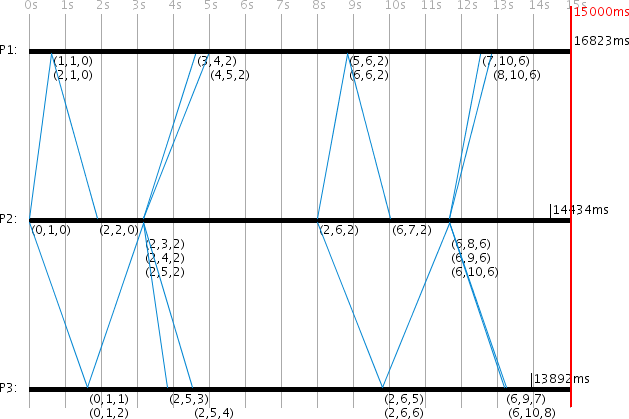
\includegraphics[width=10cm]{images/ss-protokoll-berkeley-vektor}}
	\caption{Vektorzeitstempel}
	\label{fig:Vektorzeit}
\end{figure}

Bei den Vektor-Zeitstempeln sieht es hier jedoch anders aus. Mit aktivierter Vektorzeit-Checkbox werden, wie auf Abbildung \ref{fig:Vektorzeit},  alle Vektor-Zeitstempel angezeigt.


\chapter{Protokolle und Beispiele}

Im Folgenden werden alle verf�gbaren Protokolle behandelt. Wie bereits beschrieben wird bei Protokollen zwischen Server- und Clientseite unterschieden. Server k�nnen auf Clientnachrichten, und Clients auf Servernachrichten antworten. Jeder Prozess kann beliebig viele Protokolle sowohl clientseitig als auch serverseitig unterst�tzen. Theoretisch ist es auch m�glich, dass ein Prozess f�r ein bestimmtes Protokoll gleichzeitig der Server und der Client ist. Der Anwender kann auch weitere eigene Protokolle in der Programmiersprache Java mittels der simulatoreigenen API (Application Programming Interface) erstellen (s. Kap. 4.4.4.).  
Im Programmverzeichnis des Simulators befindet sich das Verzeichnis \textit{saved-simulations} mit Beispielsimulationen. Diese liegen jeweils als serialisierter plattformunabh\"{a}ngiger Java-Bytecode in \textit{.dat}-Dateien vor. Alle Protokolle, bis auf das Beispiel-, Ping Pong- sowie das Broadcast-Protokoll, orientieren sich an den in \cite{Tanenbaum} und \cite{Vorlesung} behandelten Protokollen.

\section{Beispiel (Dummy) Protokoll}

Das Dummy-Protokoll dient lediglich als Vorlage f�r die Erstellung eigener Protokolle. Bei der Verwendung des Dummy-Protokolls werden bei Auftreten von Ereignissen (s. Kap. 2.2.3.) lediglich Lognachrichten ausgegeben. Es werden aber keine weiteren Aktionen ausgef�hrt.

\newpage
\section{Das Ping-Pong Protokoll \small{\textit{(ping-pong.dat, ping-pong-sturm.dat)}}}

\begin{figure}[h]
	\centering
	\fbox{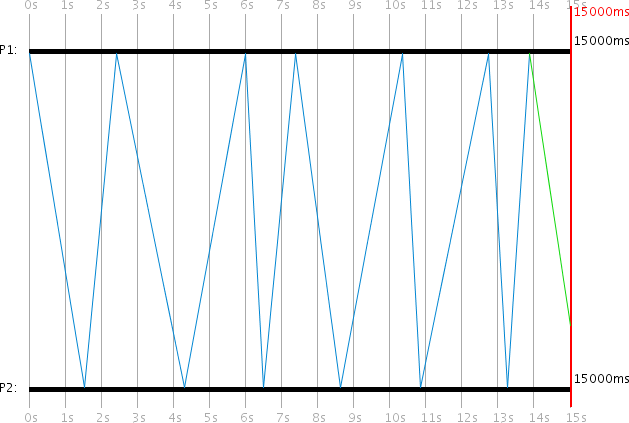
\includegraphics[width=10cm]{images/ss-protokoll-ping-pong}}
	\caption{Das Ping-Pong Protokoll}
	\label{fig:PingPongProto}
\end{figure}

Bei dem Ping-Pong Protokoll (s. Abb. \ref{fig:PingPongProto}.) werden zwischen zwei Prozessen, Client P1 und Server P2, st�ndig Nachrichten hin- und hergeschickt. Der Ping-Pong Client startet die erste Anfrage, worauf der Server dem Client antwortet. Auf diese Antwort wird vom Client ebenfalls geantwortet und so weiter. Jeder Nachricht wird ein Z�hler mitgeschickt, der bei jeder Station um eins inkrementiert- und jeweils im Logfenster protokolliert wird. In Tabelle \ref{tb:PingPongTasks}. sind alle f�r dieses Beispiel programmierten Ereignisse aufgef�hrt. 

\begin{figure}[h]
	\centering
	\fbox{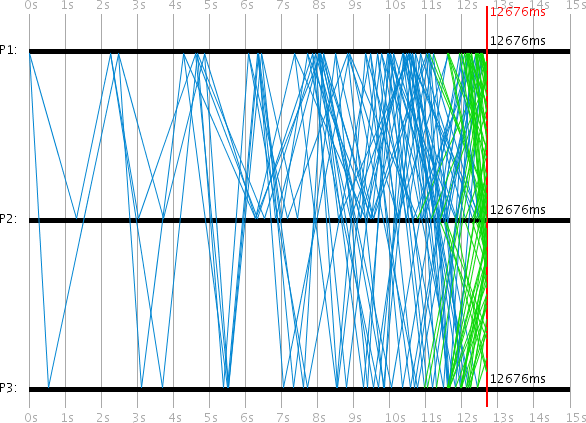
\includegraphics[width=10cm]{images/ss-protokoll-ping-pong-sturm}}
	\caption{Das Ping-Pong Protokoll (Sturm)}
	\label{fig:PingPongSturmProto}
\end{figure}

Wichtig ist, dass Prozess 1 seinen Ping-Pong Client aktiviert, bevor er eine Ping-Pong Clientanfrage startet. Wenn die Eintrittszeiten f�r die Aktivierung des Protokolls und das Starten der Anfrage identisch sind, ordnet der Task-Manager (s. Kap. 4.4.3.) diese Ereignisse automatisch in der richtigen Reihenfolge an. Bei nicht aktiviertem Ping-Pong Client kann P1 keine Ping-Pong Anfrage starten. Bevor ein Prozess eine Anfrage starten kann, muss er das dazugeh�rige Protokoll aktiviert haben. Entsprechend gilt dies auch f�r alle anderen Protokolle. Anhand dieses Beispiels ist erkennbar, dass die noch nicht ausgelieferte Nachrichte gr�n eingef�rbt ist w�hrend alle ausgelieferten Nachrichten bereits die Farbe Blau tragen (s. Tabelle \ref{tb:Farben}.).

Werden die Ereignisse wie in Tabelle \ref{tb:PingPongSturmTasks}. vorgegeben, so l�sst sich ein Ping-Pong Sturm realisieren. Hier wird ein neuer Prozess P3 eingef�hrt, der als zus�tzlicher Ping-Pong Server agiert. Da auf jede Clientnachricht stets zwei Serverantworten folgen, verdoppelt sich bei jedem Ping-Pong Durchgang die Anzahl der Nachrichten. In Abbildung \ref{fig:PingPongSturmProto}. ist der dazugeh�rige Simulationsverlauf bis zum Zeitpunkt \textit{12676ms} dargestellt.

\begin{table}
	\centering
	\fbox{
	\begin{tabular}{c|c|l}
		\textbf{Zeit (ms)} & \textbf{PID} & \textbf{Ereignis} \\
		\hline 
		 	0 & 1 & Ping Pong Client aktivieren\\
		 	0 & 2 & Ping Pong Server aktivieren\\
		 	0 & 1 & Ping Pong Clientanfrage starten
	\end{tabular}
	}
	\caption{Programmierte Ping-Pong Ereignisse}
	\label{tb:PingPongTasks}
\end{table}

\begin{table}
	\centering
	\fbox{
	\begin{tabular}{c|c|l}
		\textbf{Zeit (ms)} & \textbf{PID} & \textbf{Ereignis} \\
		\hline 
		 	0 & 1 & Ping Pong Client aktivieren\\
		 	0 & 2 & Ping Pong Server aktivieren\\
		 	0 & 3 & Ping Pong Server aktivieren\\
		 	0 & 1 & Ping Pong Clientanfrage starten
	\end{tabular}
	}
	\caption{Programmierte Ping-Pong Ereignisse (Sturm)}
	\label{tb:PingPongSturmTasks}
\end{table}

\begin{table}
	\centering
	\fbox{
	\begin{tabular}{c|c|l}
		\textbf{Zeit (ms)} & \textbf{PID} & \textbf{Ereignis} \\
		\hline 
		 	0000 & 1 & Broadcast Client aktivieren\\
		 	0000 & 2 & Broadcast Client aktivieren\\
		 	0000 & 3 & Broadcast Client aktivieren\\
		 	0000 & 4 & Broadcast Client aktivieren\\
		 	0000 & 5 & Broadcast Client aktivieren\\
		 	0000 & 6 & Broadcast Client aktivieren\\
		 	0000 & 1 & Broadcast Server aktivieren\\
		 	0000 & 2 & Broadcast Server aktivieren\\
		 	0000 & 3 & Broadcast Server aktivieren\\
		 	0000 & 4 & Broadcast Server aktivieren\\
		 	0000 & 5 & Broadcast Server aktivieren\\
		 	0000 & 6 & Broadcast Server aktivieren\\
		 	0000 & 1 & Broadcast Clientanfrage starten\\
		 	2500 & 1 & Broadcast Clientanfrage starten
	\end{tabular}
	}
	\caption{Programmierte Broadcast Ereignisse}
	\label{tb:BroadcastSturmTasks}
\end{table}
\section{Das Broadcast Protokoll \small{\textit{(broadcast.dat)}}}

\begin{figure}[h]
	\centering
	\fbox{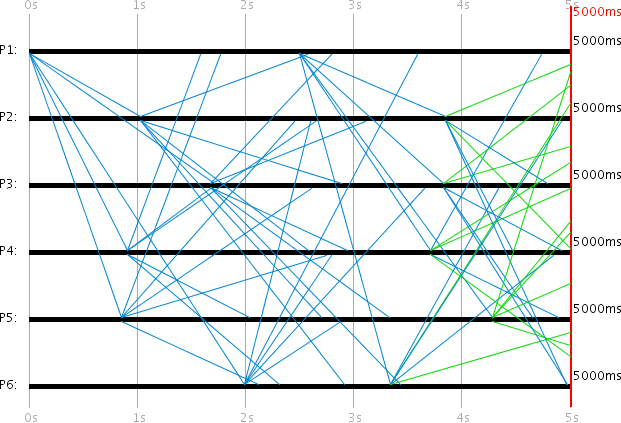
\includegraphics[width=10cm]{images/ss-protokoll-broadcast-sturm}}
	\caption{Das Broadcast Protokoll}
	\label{fig:BroadcastSturmProto}
\end{figure}

Das Broadcast Protokoll verh�lt sich �hnlich wie das Ping-Pong Protokoll. Der Unterschied ist, dass sich das Protokoll anhand einer eindeutigen Broadcast-ID merkt, welche Nachrichten bereits verschickt wurden. Jeder Prozess verschickt beim Broadcast Protokoll alle erhaltenen Nachrichten erneut, sofern er sie noch nicht schon einmal verschickt hat. 

In diesem Fall wird nicht zwischen Client und Server unterschieden, so dass bei der Ankunft einer Nachricht jeweils die gleiche Aktion durchgef\"{u}hrt wird. Somit l�sst sich, unter Verwendung mehrerer Prozesse (s. Abb. \ref{fig:BroadcastSturmProto}.) ein Broadcast erzeugen. P1 ist der Client und startet je eine Anfrage nach \textit{0ms} und \textit{2500ms}. Die Simulationsdauer betr�gt hier genau \textit{5000ms}. Da ein Client nur Servernachrichten und ein Server nur Clientnachrichten empfangen kann, ist in dieser Simulation jeder Prozess (s. Tabelle \ref{tb:BroadcastSturmTasks}) gleichzeitig Server und Client. 


\section{Das Protokoll zur internen Synchronisierung in einem synchronen System \small{\textit{(int-sync.dat)}}}

Bisher wurden nur Protokolle dargestellt, in denen die beteiligten Prozesse keine Uhrabweichungen hatten. Das Protokoll zur internen Synchronisierung ist ein Protokoll zur Synchronisierung der lokalen Prozesszeit, welches beispielsweise angewendet werden kann, wenn eine Prozesszeit aufgrund einer Uhrabweichung falsch geht. Wenn der Client seine (falsche) lokale Prozesszeit $t_c$ mit einem Server synchronisieren m�chte, so schickt er ihm eine Clientanfrage. Der Server schickt als Antwort seine eigene lokale Prozesszeit $t_s$ zur�ck, womit der Client eine neue und genauere Prozesszeit f\"{u}r sich berechnen kann. Die neue Prozesszeit wird wie folgt berechnet:

\begin{figure}[h]
	\centering
	\fbox{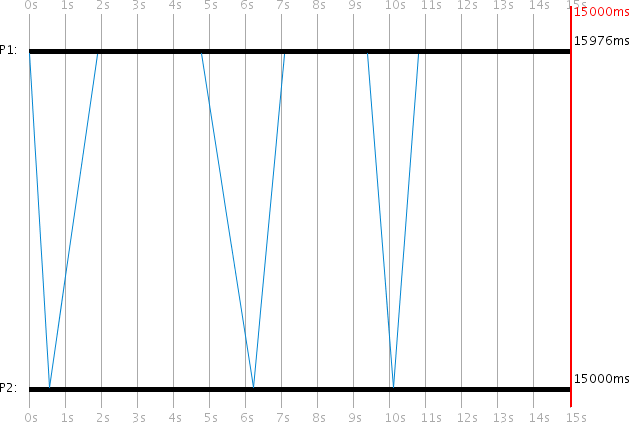
\includegraphics[width=10cm]{images/ss-protokoll-time-sync}}
	\caption{Das Protokoll zur internen Synchronisierung}
	\label{fig:TimeSyncProto}
\end{figure}

Hier (s. Abb. \ref{fig:TimeSyncProto}.) stellt P1 den Client und P2 den Server dar. Da die �bertragungszeit $t_u$ einer Nachricht zwischen den vermuteten Werten $t'_{min}$ und $t'_{max}$ liegt, berechnet der Client P1 nach Empfang der Serverantwort seine neue lokale Prozesszeit mit:

\begin{equation*}
	t_c := t_s + \frac{1}{2} (t'_{min} + t'_{max})
\end{equation*}

Somit wird die lokale Zeit von P1, mit einem Fehler von $< \frac{1}{2} (t'_{max} - t'_{min})$, mit der Serverzeit synchronisiert (siehe \cite{Vorlesung}). 

Im Beispiel hat der Clientprozess als Uhrabweichung den Wert \textit{0.1} und der Server hat als Uhrabweichung den Wert \textit{0.0} konfiguriert. Der Client startet, wie in Tabelle \ref{tb:InterneSyncTasks}. angegeben, nach \textit{0ms}, \textit{5000ms} und \textit{10000ms} seiner lokalen Prozesszeit jeweils eine Clientanfrage. In der Abbildung l�sst sich erkennen, dass die zweite und die dritte Anfrage nicht synchron zu der globalen Zeit (vgl. Sekunden-Zeitgatter, Abbildung \ref{tb:TimeSyncProto)}.) gestartet wurden, was auf die Uhrabweichung von P1 zur�ckzuf�hren ist. Nach Simulationsende ist die Zeit von P1 bis auf \textit{15000ms} - \textit{15976ms} = \textit{-976ms} synchronisiert.

\begin{table}
	\centering
	\fbox{
	\begin{tabular}{c|c|l}
		\textbf{Zeit (ms)} & \textbf{PID} & \textbf{Ereignis} \\
		\hline 
		 	00000 & 1 & Interne Sync. Client aktivieren \\
		 	00000 & 2 & Interne Sync. Server aktivieren\\
		 	00000 & 1 & Interne Sync. Clientanfrage starten\\
		 	05000 & 1 & Interne Sync. Clientanfrage starten\\
		 	10000 & 1 & Interne Sync. Clientanfrage starten\\
	\end{tabular}
	}
	\caption{Programmierte Ereignisse zur internen Synchronisierung}
	\label{tb:InterneSyncTasks}
\end{table}

\subsubsection{Protokollvariablen}

Dieses Protokoll verwendet folgende zwei clientseitige Variablen, die in den Prozesseinstellungen unter dem Punkt ``Interne Sync. Client'' konfiguriert werden k�nnen. Serverseitig gibt es hier keine Variablen.

\begin{itemize}
	\item \textbf{Min. �bertragungszeit} \textit{(Long: 500)}: Gibt den Wert $t'_{min}$ in Millisekunden an
	\item \textbf{Max. �bertragungszeit} \textit{(Long: 2000)}: Gibt den Wert $t'_{max}$ in Millisekunden an
\end{itemize}

$t'_{min}$ und $t'_{max}$ sind die bei den Protokollberechnungen verwendeten Werte. Sie k�nnen sich allerdings von den tats�chlichen Nachrichten�bertragungszeiten $t_{min}$ und $t_{max}$ (s. Kap. 2.4.3.) unterscheiden. Somit lassen sich auch Szenarien simulieren, in denen das Protokoll falsch eingestellt wurde und wobei der Zeitsynchronisierung gro�e Fehler auftreten k�nnen.


\section{Christians Methode zur externen Synchronisierung \small{\textit{(ext-vs-int-sync.dat)}}}

\begin{figure}[h]
	\centering
	\fbox{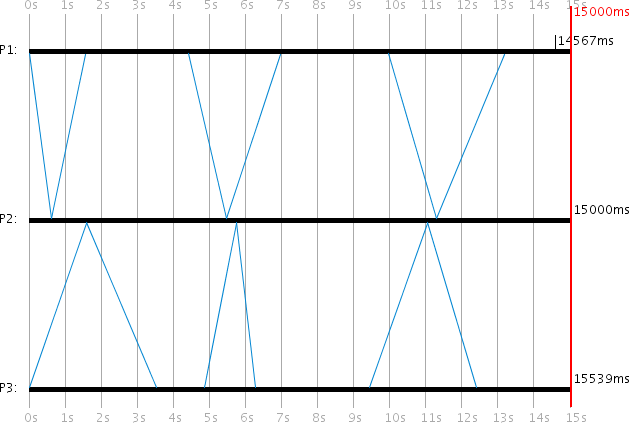
\includegraphics[width=10cm]{images/ss-protokoll-time-sync-2}}
	\caption{Interne Synchronisierung und Christians Methode im Vergleich}
	\label{fig:TimeSync2Proto}
\end{figure}

Ein weiteres Protokoll f�r die Synchronisierung von Uhrzeiten funktioniert nach der Christians Methode zur externen Synchronisierung. Die Christians Methode benutzt die RTT (Round Trip Time) $t_{rtt}$, um die �bertragungszeit von einzelnen Nachrichten zu approximieren. 

Wenn der Client seine lokale Zeit $t_c$ bei einem Server synchronisieren m�chte, so verschickt er eine Anfrage, und misst dabei die dazugeh�rige RTT $t_{rtt}$ bis zur Ankunft der Serverantwort. Die Serverantwort beinhaltet die lokale Prozesszeit $t_s$ des Servers von dem Zeitpunkt an dem der Server die Antwort verschickt. Der Client berechnet dann seine lokale Zeit neu mit:

\begin{equation*}
	t_c := t_s + \frac{1}{2} t_{rtt}
\end{equation*}

Die Genauigkeit betr\"{a}gt $\pm(\frac{1}{2} t_{rtt} - u_{min}$) wobei $u_{min}$ mit $t_{rtt} < u_{min}$ eine Schranke f�r eine Nachrichten�bertragung darstellt(s. \cite{Vorlesung}).

Im Prinzip sieht der Verlauf einer Christians-Simulation so aus wie in Abbildung \ref{fig:TimeSyncProto}., daher wird hier auf eine einfache Abbildung vom Christians-Protokoll verzichtet. Viel interessanter ist der direkte Vergleich zwischen dem Protokoll zur internen Synchronisierung und der Christians Methode der externen Synchronisierung (s. Abb. \ref{fig:TimeSync2Proto}.). Hier stellt P1 den Client zur internen Synchronisierung und P3 den Client zur externen Synchronisierung dar. P2 fungiert f�r beide Protokolle gleichzeitig als Server. P1 und P3 starten jeweils zu den lokalen Prozesszeiten \textit{0ms}, \textit{5000ms} und \textit{10000ms} eine Clientanfrage (s. Tabelle \ref{tb:InterneSync2Tasks}.). P1 und P3 haben als Uhrabweichung einen Wert von \textit{0.1} eingestellt und die Simulationsdauer betr�gt insgesamt \textit{15000ms}.

Aus Abbildung \ref{fig:TimeSync2Proto}. ist ersichtlich, dass nach Ablauf der Simulation, P1 seine Zeit bis auf \textit{15000ms} - \textit{14567ms} = \textit{433ms} und P3 seine Zeit bis auf \textit{15000ms} - \textit{15539ms} = \textit{-539ms} synchronisiert hat. In diesem Beispiel hat also das Protokoll zur internen Synchronisierung ein besseres Ergebnis geliefert. Dies ist allerdings nicht immer zwingend der Fall, da nach einer erneuten Simulationsausf�hrung alle Nachrichten jeweils eine neue zuf�llige �bertragungszeit zwischen $t_{min}$ und $t_{max}$ haben werden, die auf die Zeitsynchronisation mit den einem oder anderem Protokoll jeweils andere Auswirkungen haben k\"{o}nnen. 

\begin{table}
	\centering
	\fbox{
	\begin{tabular}{c|c|l}
		\textbf{Zeit (ms)} & \textbf{PID} & \textbf{Ereignis} \\
		\hline 
		 	00000 & 1 & Interne Sync. Client aktivieren \\
		 	00000 & 1 & Interne Sync. Clientanfrage starten\\
		 	00000 & 2 & Christians Server aktivieren\\
		 	00000 & 2 & Interne Sync. Server aktivieren\\
		 	00000 & 3 & Christians Client aktivieren \\
		 	00000 & 3 & Christians Clientanfrage starten\\
		 	05000 & 1 & Interne Sync. Clientanfrage starten\\
		 	05000 & 3 & Christians Clientanfrage starten\\
		 	10000 & 1 & Interne Sync. Clientanfrage starten\\
		 	10000 & 3 & Christians Clientanfrage starten\\
	\end{tabular}
	}
	\caption{Programmierte Ereignisse, Vergleich interner und externer Synchronisierung}
	\label{tb:InterneSync2Tasks}
\end{table}

\section{Der Berkeley Algorithmus zur internen Synchronisierung \small{\textit{(berkeley.dat)}}}

\begin{figure}[h]
	\centering
	\fbox{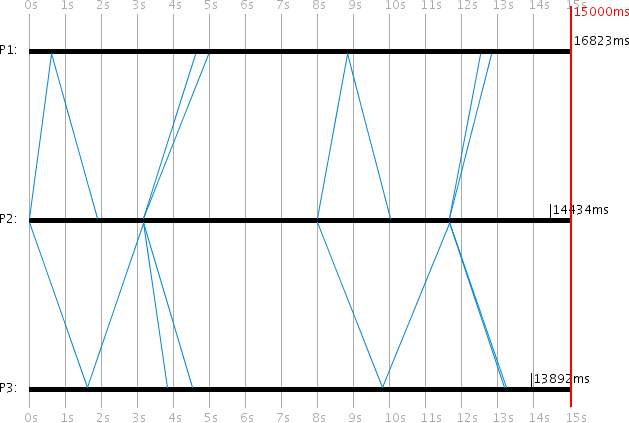
\includegraphics[width=10cm]{images/ss-protokoll-berkeley}}
	\caption{Der Berkeley Algorithmus zur internen Synchronisierung}
	\label{fig:BerkeleyProto}
\end{figure}

Der Berkeley Algorithmus zur internen Synchronisierung ist eine weitere M�glichkeit lokale Uhrzeiten abzugleichen. Dies ist das erste Protokoll, wo der Server die Anfragen startet. Der Server fungiert gewisserma�en Koordinator des Protokolls. Die Clientprozesse sind somit passiv und m�ssen warten, bis eine Serveranfrage eintrifft. Hierbei muss der Server wissen, welche Clientprozesse an dem Protokoll teilnehmen, was sich in den Protokolleinstellungen des Servers einstellen l�sst (s. Kap. 2.4.3.).

Wenn der Server seine lokale Zeit $t_s$ und auch die Prozesszeiten $t_i$ der Clients ($i = 1, ..., n$) synchronisieren m�chte, so verschickt er eine Serveranfrage. $n$ sei hierbei die Anzahl beteiligter Clients. Die Clients senden dann ihre lokalen Prozesszeiten in einer Nachricht zur�ck zum Server. Der Server hat dabei die RTTs $r_i$ bis zur Ankunft aller Clientantworten gemessen. 

Nachdem alle Antworten vorliegen, setzt er zun�chst seine eigene Zeit $t_s$ auf den Mittelwert $t_{avg}$ aller bekannten Prozesszeiten (seiner eigenen Prozesszeit eingeschlossen). Die �bertragungszeit einer Clientantwort wird auf die H�lfte der RTT gesch�tzt und in der Berechnung von $t_{avg}$ wie folgt ber�cksichtigt: 
\begin{equation*}
	t_{avg} :=
	\frac{1}{n+1} ( t_s +
		\sum_{\substack{
			i=1\\
		}}^n
		\frac{r_i}{2} + t_i
	)
\end{equation*}
\begin{equation*}
	t_s := t_{avg}
\end{equation*}

Anschlie�end berechnet der Server f�r jeden Client einen Korrekturwert $k_i := t_{avg} - t_i$, den er jeweils in einer separaten Nachricht an die einzelnen Clients zur�ckschickt. Diese setzten dann jeweils die lokalen Prozesszeiten auf $t'_i := t'_i + k_i$. Wobei $t'_i$ die lokale, aktuelle Prozesszeit des jeweiligen Clients ist. 

Im Beispiel in Abbildung \ref{fig:BerkeleyProto}. gibt es die 2 Clientprozesse P1 und P3 sowie den Serverprozess P2. Der Server startet nach jeweils \textit{0ms} und \textit{7500ms} eine Synchronisierungsanfrage (s. Tabelle \ref{tb:BerkeleyTasks}.). Hier f�llt auf, dass der Server stets 2 Korrekturwerte verschickt, die jeweils P1 und P3 erreichen. Es werden hier also pro Synchronisierungsvorgang insgesamt 4 Korrekturwerte ausgeliefert. Eine Korrekturnachricht enth�lt neben dem Korrekturwert $k_i$ auch die PID des Prozesses, f�r den die Nachricht bestimmt ist. Indem das Protokoll die PID �berpr�ft verarbeitet ein Client so nur die f�r ihn bestimmten Korrekturwerte.

\begin{table}
	\centering
	\fbox{
	\begin{tabular}{c|c|l}
		\textbf{Zeit (ms)} & \textbf{PID} & \textbf{Ereignis} \\
		\hline 
		 	0000 & 1 & Berkeley Client aktivieren \\
		 	0000 & 2 & Berkeley Server aktivieren \\
		 	0000 & 3 & Berkeley Client aktivieren \\
		 	0000 & 2 & Berkeley Serveranfrage starten\\
		 	7500 & 2 & Berkeley Serveranfrage starten\\
	\end{tabular}
	}
	\caption{Programmierte Ereignisse zum Berkeley Algorithmus}
	\label{tb:BerkeleyTasks}
\end{table}
\subsubsection{Protokollvariablen}

Dieses Protokoll verwendet folgende serverseitige Variable, die in den Prozesseinstellungen unter dem Punkt ``Berkeley Server'' konfiguriert werden kann. Clientseitig gibt es hierbei keine Einstellungsm\"{o}glichkeiten.

\begin{itemize}
	\item \textbf{PIDs beteiligter Prozesse} \textit{(Integer[]: [1,3])}: Dieser Vektor aus Integerwerten beinhaltet alle PIDs der Berkeley Clientprozesse, mit denen der Berkeley Server die Zeit synchronisieren soll. Das Protokoll funktioniert nicht, wenn hier eine PID angegeben wird die nicht existiert oder die das Berkeley Protokoll clientseitig nicht unterst�tzt. In diesem Fall w�rde ewig auf eine (fehlende) Clientantwort gewartet werden.
\end{itemize}

\section{Das Ein-Phasen Commit Protokoll \small{\textit{(one-phase-commit.dat)}}}

\begin{figure}[h]
	\centering
	\fbox{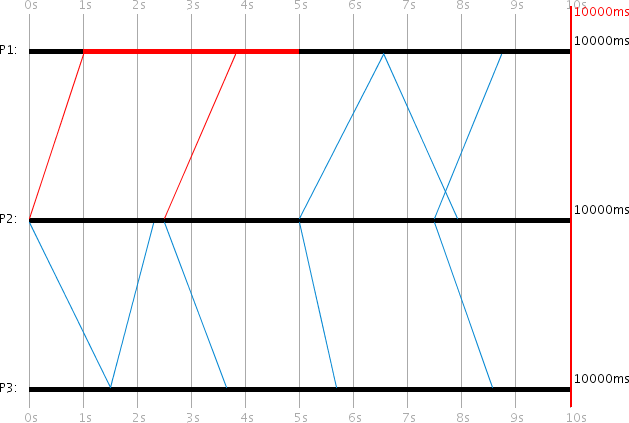
\includegraphics[width=10cm]{images/ss-protokoll-one-phase-commit}}
	\caption{Das Ein-Phasen Commit Protokoll}
	\label{fig:OnePhaseCommitProto}
\end{figure}

Das Ein-Phasen Commit Protokoll ist daf�r gedacht beliebig vielen Clients zu einer Festschreibung zu bewegen. Im realen Leben k�nnte dies beispielsweise das Erstellen oder L�schen einer Datei sein, von der auf jedem Client eine lokale Kopie existiert. Der Server ist der Koordinator und auch derjenige, der einen Festschreibewunsch initiiert. Hierbei verschickt der Server periodisch so oft den Festschreibewunsch, bis er von jedem Client eine Best�tigung erhalten hat. Hierf\"{u}r m\"{u}ssen f\"{u}r den Server die PIDs aller beteiligten Clientprozesse sowie ein Wecker f\"{u}r erneutes Versenden des Festschreibewunsches konfiguriert werden.

Die programmierten Ereignisse des Beispiels auf (s. Abb. \ref{fig:OnePhaseCommitProto}.) sind in Tabelle \ref{tb:OnePhaseCommitTasks}. aufgelistet. P1 und P3 simulieren jeweils einen Client und P2 den Server. Damit die Simulation mehrere Festschreibew�nsche verschickt, st�rzt in der Simulation P1 nach \textit{1000ms} ab und nach \textit{5000ms} steht er wieder zur Verf�gung. Die ersten beide Festschreibew�nsche erreichen dadurch P1 nicht und erst der dritte Versuch verl�uft erfolgreich. Bevor die Best�tigung von P1 bei P2 eintrifft, l�uft jedoch der Wecker erneut ab, so dass ein weiterer Festschreibewunsch versendet wird. Da P1 und P3 jeweils schon eine Best�tigung verschickt haben, wird diese Festschreibewunschnachricht ignoriert. Jeder Client best�tigt auf einen Festschreibewunsch nur ein einziges Mal.

\begin{table}
	\centering
	\fbox{
	\begin{tabular}{c|c|l}
		\textbf{Zeit (ms)} & \textbf{PID} & \textbf{Ereignis} \\
		\hline 
		 	0000 & 1 & 1-Phasen Commit Client aktivieren\\
		 	0000 & 2 & 1-Phasen Commit Server aktivieren\\
		 	0000 & 3 & 1-Phasen Commit Client aktivieren\\
		 	0000 & 2 & 1-Phasen Commit Serveranfrage starten\\
		 	1000 & 1 & Prozessabsturz\\
		 	5000 & 1 & Prozesswiederbelebung
	\end{tabular}
	}
	\caption{Programmierte Ein-Phasen Commit Ereignisse}
	\label{tb:OnePhaseCommitTasks}
\end{table}

\subsubsection{Protokollvariablen}

Dieses Protokoll verwendet folgende serverseitige Variablen, die in den Prozesseinstellungen unter dem Punkt ``1-Phasen Commit Server'' konfiguriert werden k�nnen. Clientseitig gibt es hier keine Variablen.

\begin{itemize}
	\item \textbf{Zeit bis erneute Anfrage} \textit{(Long: timeout = 2500)}: Gibt die Anzahl von Millisekunden an, die gewartet werden sollen, bis der Festschreibewunsch erneut verschickt wird.
	\item \textbf{PIDs beteiligter Prozesse} \textit{(Integer[]: pids = [1,3])}: Dieser Vektor aus Integerwerten beinhaltet alle PIDs der Clientprozesse, die festschreiben sollen. 
\end{itemize}


\section{Das Zwei-Phasen Commit Protokoll \small{\textit{(two-phase-commit.dat)}}}

\begin{figure}[h]
	\centering
	\fbox{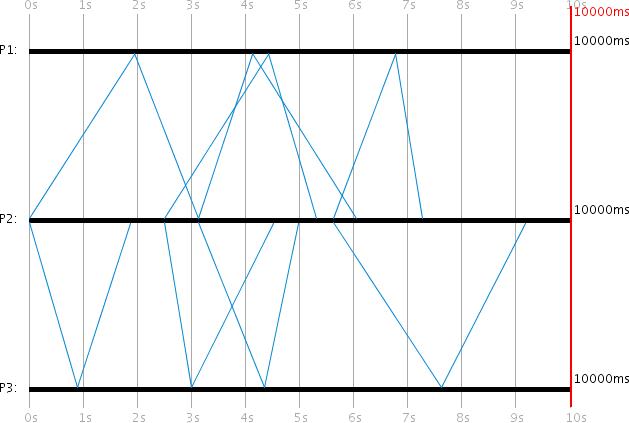
\includegraphics[width=10cm]{images/ss-protokoll-two-phase-commit}}
	\caption{Das Zwei-Phasen Commit Protokoll}
	\label{fig:TwoPhaseCommitProto}
\end{figure}

Das Zwei-Phasen Commit Protokoll ist eine Erweiterung des Ein-Phasen Commit Protokolls. Der Server startet zun�chst eine Anfrage an alle beteiligten Clients, ob festgeschrieben werden soll. Jeder Client antwortet dann mit \textit{true} oder \textit{false}. Der Server fragt periodisch so oft nach, bis alle Ergebnisse aller Clients vorliegen. Nach Erhalt aller Abstimmungen �berpr�ft der Server, ob alle mit \textit{true} abgestimmt haben. F�r den Fall dass mindestens ein Client mit \textit{false} abgestimmt hat, wird der Festschreibevorgang abgebrochen und als globales Abstimmungsergebnis \textit{false} an alle Clients verschickt. Wenn jedoch alle mit \textit{true} abstimmten, soll festgeschrieben werden. Dabei wird das globale Abstimmungsergebnis \textit{true} verschickt. Das globale Abstimmungsergebnis wird periodisch so oft erneut verschickt, bis von jedem Client eine Best�tigung des Erhalts vorliegt.

In dem Beispiel (s. Abb. \ref{fig:TwoPhaseCommitProto}.) sind P1 und P3 Clients und P2 der Server. Der Server verschickt nach \textit{0ms} seine erste Anfrage (s. Tabelle \ref{tb:TwoPhaseCommitTasks}.). Da diese Simulation recht un�bersichtlich ist, liegen in den Tabellen \ref{tb:TwoPhaseCommitLogs}. und \ref{tb:TwoPhaseCommitLogs2}. Ausz�ge aus dem Logfenster vor. Die Lamport- und Vektor-Zeitstempel sowie die lokalen Prozesszeiten sind hier nicht aufgef\"{u}hrt. Da keine Uhrabweichungen konfiguriert wurden, sind die lokalen Prozesszeiten stets identisch mit der globalen Zeit, weswegen in den Tabellen pro Logeintrag jeweils nur eine Zeit angegeben ist. Anhand der Nachrichten IDs lassen sich dort die einzelnen Sendungen zuordnen. In den Logs wird auch der Inhalt der verschickten Nachricht sowie die dazugeh�rigen Datentypen aufgef�hrt. Hier stimmen P1 und P3 jeweils mit \textit{true} ab, das hei�t es soll festgeschrieben werden. 

\begin{table}
	\centering
	\fbox{
	\begin{tabular}{c|c|l}
		\textbf{Zeit (ms)} & \textbf{PID} & \textbf{Ereignis} \\
		\hline 
		 	0000 & 1 & 2-Phasen Commit Client aktivieren\\
		 	0000 & 2 & 2-Phasen Commit Server aktivieren\\
		 	0000 & 3 & 2-Phasen Commit Client aktivieren\\
		 	0000 & 2 & 2-Phasen Commit Serveranfrage starten
	\end{tabular}
	}
	\caption{Programmierte Zwei-Phasen Commit Ereignisse}
	\label{tb:TwoPhaseCommitTasks}
\end{table}

\subsubsection{Protokollvariablen}

Dieses Protokoll verwendet folgende serverseitige Variablen, die in den Prozesseinstellungen unter dem Punkt ``2-Phasen Commit Server'' konfiguriert werden k�nnen:

\begin{itemize}
	\item \textbf{Zeit bis erneute Anfrage} \textit{(Long: timeout = 2500)}: Gibt die Anzahl von Millisekunden an, die gewartet werden sollen, bis der Festschreibewunsch erneut verschickt wird.
	\item \textbf{PIDs beteiligter Prozesse} \textit{(Integer[]: pids = [1,3])}: Dieser Vektor aus Integerwerten beinhaltet alle PIDs der Clientprozesse die �ber eine Festschreibung abstimmen und anschlie�end gegebenenfalls festschreiben sollen. 
\end{itemize}

Die folgende Clientvariable kann unter den Prozesseinstellungen unter dem Punkt ``2-Phasen Commit Client'' konfiguriert werden:

\begin{itemize}
	\item \textbf{Festschreibwahrscheinlichkeit} \textit{(Integer: ackProb = 50)}: Gibt die Wahrscheinlichkeit in Prozent an, die der Client mit \textit{true}, also f�r das Festschreiben, abstimmt.
\end{itemize}

\begin{table}
	\centering
	\fbox{
	\begin{tabular}{c|c|l}
		\textbf{Zeit (ms)} & \textbf{PID} & \textbf{Lognachricht} \\
			\hline
000000 & & Simulation gestartet\\
\hline
000000 & 1 & 2-Phasen Commit Client aktiviert\\
\hline
000000 & 2 & 2-Phasen Commit Server aktiviert\\
\hline
000000 & 2 & Nachricht versendet; ID: 94; Protokoll: 2-Phasen Commit\\
	& & Boolean: wantVote=true\\
\hline
000000 & 3 & 2-Phasen Commit Client aktiviert\\
\hline
000905 & 3 & Nachricht erhalten; ID: 94; Protokoll: 2-Phasen Commit\\
\hline
000905 & 3 & Nachricht versendet; ID: 95; Protokoll: 2-Phasen Commit\\
	& & Integer: pid=3; Boolean: isVote=true; vote=true\\
\hline
000905 & 3 & Abstimmung true versendet\\
\hline
001880 & 2 & Nachricht erhalten; ID: 95; Protokoll: 2-Phasen Commit\\
\hline
001880 & 2 & Abstimmung von Prozess 3 erhalten! Ergebnis: true\\
\hline
001947 & 1 & Nachricht erhalten; ID: 94; Protokoll: 2-Phasen Commit\\
\hline
001947 & 1 & Nachricht versendet; ID: 96; Protokoll: 2-Phasen Commit\\
	& & Integer: pid=1; Boolean: isVote=true; vote=true\\
\hline
001947 & 1 & Abstimmung true versendet\\
\hline
002500 & 2 & Nachricht versendet; ID: 97; Protokoll: 2-Phasen Commit\\
	& & Boolean: wantVote=true\\
\hline
003006 & 3 & Nachricht erhalten; ID: 97; Protokoll: 2-Phasen Commit\\
\hline
003006 & 3 & Nachricht versendet; ID: 98; Protokoll: 2-Phasen Commit\\
	& & Integer: pid=3; Boolean: isVote=true; vote=true\\
\hline
003006 & 3 & Abstimmung true versendet\\
\hline
003137 & 2 & Nachricht erhalten; ID: 96; Protokoll: 2-Phasen Commit\\
\hline
003137 & 2 & Abstimmung von Prozess 1 erhalten! Ergebnis: true\\
\hline
003137 & 2 & Abstimmungen von allen beteiligten Prozessen erhalten!\\
	& & Globales Ergebnis: true\\
\hline
003137 & 2 & Nachricht versendet; ID: 99; Protokoll: 2-Phasen Commit\\
	& & Boolean: isVoteResult=true; voteResult=true\\
\hline
004124 & 1 & Nachricht erhalten; ID: 99; Protokoll: 2-Phasen Commit\\
\hline
004124 & 1 & Globales Abstimmungsergebnis erhalten. Ergebnis: true\\
\hline
004124 & 1 & Nachricht versendet; ID: 100; Protokoll: 2-Phasen Commit\\
	& & Integer: pid=1; Boolean: isAck=true\\
\hline
004354 & 3 & Nachricht erhalten; ID: 99; Protokoll: 2-Phasen Commit\\
\hline
004354 & 3 & Globales Abstimmungsergebnis erhalten. Ergebnis: true\\
\hline
004354 & 3 & Nachricht versendet; ID: 101; Protokoll: 2-Phasen Commit\\
	& & Integer: pid=3; Boolean: isAck=true\\
\hline
004434 & 1 & Nachricht erhalten; ID: 97; Protokoll: 2-Phasen Commit\\
\hline
004434 & 1 & Nachricht versendet; ID: 102; Protokoll: 2-Phasen Commit\\
	& & Integer: pid=1; Boolean: isVote=true; vote=true\\
	\end{tabular}
	}
	\caption{Auszug aus dem Logfenster des Zwei-Phasen Commit Beispiels}
	\label{tb:TwoPhaseCommitLogs}
\end{table}

\begin{table}
	\centering
	\fbox{
	\begin{tabular}{c|c|l}
		\textbf{Zeit (ms)} & \textbf{PID} & \textbf{Lognachricht} \\
			\hline
004434 & 1 & Abstimmung true versendet\\
\hline
004527 & 2 & Nachricht erhalten; ID: 98; Protokoll: 2-Phasen Commit\\
\hline
004975 & 2 & Nachricht erhalten; ID: 101; Protokoll: 2-Phasen Commit\\
\hline
005311 & 2 & Nachricht erhalten; ID: 102; Protokoll: 2-Phasen Commit\\
\hline
005637 & 2 & Nachricht versendet; ID: 103; Protokoll: 2-Phasen Commit\\
	& & Boolean: isVoteResult=true; voteResult=true\\
\hline
006051 & 2 & Nachricht erhalten; ID: 100; Protokoll: 2-Phasen Commit\\
\hline
006051 & 2 & Alle Teilnehmer haben die Abstimmung erhalten\\
\hline
006766 & 1 & Nachricht erhalten; ID: 103; Protokoll: 2-Phasen Commit\\
\hline
006766 & 1 & Globales Abstimmungsergebnis erhalten. Ergebnis: true\\
\hline
006766 & 1 & Nachricht versendet; ID: 104; Protokoll: 2-Phasen Commit\\
	& & Integer: pid=1; Boolean: isAck=true\\
\hline
007279 & 2 & Nachricht erhalten; ID: 104; Protokoll: 2-Phasen Commit\\
\hline
007618 & 3 & Nachricht erhalten; ID: 103; Protokoll: 2-Phasen Commit\\
\hline
007618 & 3 & Globales Abstimmungsergebnis erhalten. Ergebnis: true\\
\hline
007618 & 3 & Nachricht versendet; ID: 105; Protokoll: 2-Phasen Commit\\
	& & Integer: pid=3; Boolean: isAck=true\\
\hline
009170 & 2 & Nachricht erhalten; ID: 105; Protokoll: 2-Phasen Commit\\
\hline
010000 & & Simulation beendet
	\end{tabular}
	}
	\caption{Auszug aus dem Logfenster des Zwei-Phasen Commit Beispiels (2)}
	\label{tb:TwoPhaseCommitLogs2}
\end{table}


\section{Der ungen�gende (Basic) Multicast \small{\textit{(basic-multicast.dat)}}}

\begin{figure}[h]
	\centering
	\fbox{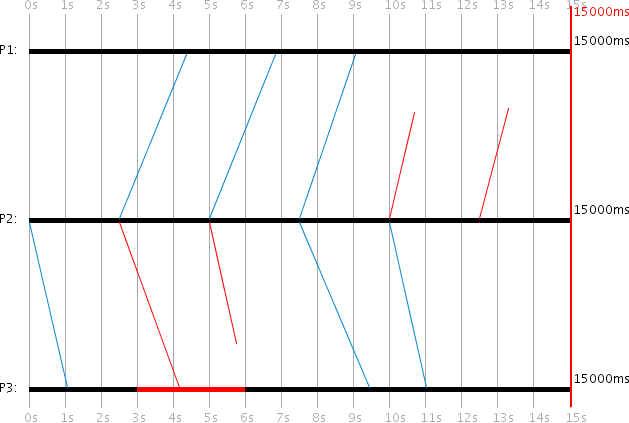
\includegraphics[width=10cm]{images/ss-protokoll-basic-multicast}}
	\caption{Das Basic-Multicast Protokoll}
	\label{fig:BasicMulticastProto}
\end{figure}

Das Basic-Multicast Protokoll ist sehr einfach aufgebaut. Im Beispiel in Abbildung \ref{fig:BasicMulticastProto}. sind P1 und P3 Server und P2 der Client. Bei diesem Protokoll startet der Client immer die Anfrage, welche bei diesem Protokoll eine einfache Multicast-Nachricht darstellt. Die Basic-Multicast Server dienen dabei lediglich zum Empfang einer Nachricht. Es werden keine Best�tigungen verschickt. Wie in Tabelle \ref{tb:BasicMulticastTasks}. aufgef�hrt verschickt P2 alle \textit{2500ms} jeweils eine Multicast-Nachricht, die alle voneinander v�llig unabh�ngig sind. 

P1 kann jedoch erst nach \textit{2500ms} Multicast-Nachrichten empfangen, da er vorher das Protokoll nicht unterst�tzt w�hrend P3 von \textit{3000ms} bis \textit{6000ms} abgest�rzt ist und in dieser Zeit auch keine Nachrichten empfangen kann. In diesem Beispiel ist P1 ein Server, der erst sp\"{a}ter ans Netz angeschlossen wird. Da die Einstellung ``Nur relevante Nachrichten anzeigen'' aktiviert ist, wird die erste Multicast-Nachricht von P2 an P1 nicht dargestellt. Bei jedem Prozess wurde die Nachrichtenverlustwahrscheinlichkeit auf \textit{30} Prozent gestellt, so dass alle in dieser Simulation verschickten Nachrichten mit einer Wahrscheinlichkeit von \textit{30} Prozent ausfallen. 

In diesem Beispiel ging die 3. Multicast-Nachricht auf den Weg zu P3- und die 5. sowie 6. Nachricht auf den Weg zu P1 verloren. Lediglich die 4. Multicast-Nachricht hat beide Ziele erreicht.

\begin{table}
	\centering
	\fbox{
	\begin{tabular}{c|c|l}
		\textbf{Zeit (ms)} & \textbf{PID} & \textbf{Ereignis} \\
		\hline 
		 	00000 & 2 & Basic Multicast Client aktivieren\\
		 	00000 & 3 & Basic Multicast Server aktivieren\\
		 	00000 & 2 & Basic Multicast Clientanfrage starten\\
		 	02500 & 1 & Basic Multicast Server aktivieren\\
		 	02500 & 2 & Basic Multicast Clientanfrage starten\\
		 	03000 & 3 & Prozessabsturz\\
		 	05000 & 2 & Basic Multicast Clientanfrage starten\\
		 	06000 & 3 & Prozesswiederbelebung\\
		 	07500 & 2 & Basic Multicast Clientanfrage starten\\
		 	10000 & 2 & Basic Multicast Clientanfrage starten\\
		 	12500 & 2 & Basic Multicast Clientanfrage starten
	\end{tabular}
	}
	\caption{Programmierte Basic-Multicast Ereignisse}
	\label{tb:BasicMulticastTasks}
\end{table}


\section{Das zuverl�ssige (Reliable) Multicast Protokoll \small{\textit{(reliable-multicast.dat)}}}

\begin{figure}[h]
	\centering
	\fbox{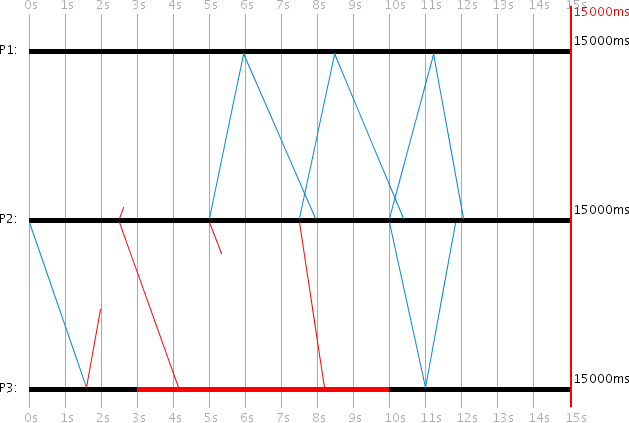
\includegraphics[width=10cm]{images/ss-protokoll-reliable-multicast}}
	\caption{Das Reliable-Multicast Protokoll}
	\label{fig:ReliableMulticastProto}
\end{figure}

Bei dem  zuverl�ssigen (Reliable) Multicast verschickt der Client periodisch so oft seine Multicast-Nachricht, bis er von allen beteiligten Servern eine Best�tigung erhalten hat. Nach jedem erneuten Versuch vergisst der Client, von welchen Servern er bereits eine Best�tigung erhalten hat, wodurch jede erneute Anfrage von allen Teilnehmern aufs Neue best\"{a}tigt werden muss. In dem Beispiel (s. Abb. \ref{fig:ReliableMulticastProto}., Tabelle \ref{tb:ReliableMulticastTasks}., \ref{tb:ReliableMulticastLogs}. und \ref{tb:ReliableMulticastLogs2}.) ist P2 der Multicast-verschickende Client, w�hrend P1 und P3 die Server darstellen. Bei \textit{0ms} initiiert der Client seine Multicast-Nachricht. Die Nachrichtenverlustwahrscheinlichkeiten sind bei allen Prozessen auf \textit{30} Prozent eingestellt.

In diesem Beispiel ben�tigt der Client bis zur erfolgreichen Auslieferung des zuverl�ssigen Multicasts genau 5 Versuche:

\begin{enumerate}
	\setlength{\itemsep}{-1mm}
	\item Versuch: 
		\begin{itemize}
			\setlength{\itemsep}{-2.5mm}
			\item P1 unterst�tzt das Reliable-Multicast Protokoll noch nicht, und kann somit weder Multicast-Nachricht erhalten noch eine Best�tigung verschicken.
			\item P3 empf�ngt die Multicast-Nachricht, jedoch geht seine Best�tigungsnachricht verloren.
		\end{itemize}
	\item Versuch: 
		\begin{itemize}
			\setlength{\itemsep}{-2.5mm}
			\item P1: Die Multicast-Nachricht geht unterwegs zu P1 verloren.
			\item P3: Die Multicast-Nachricht erreicht P3, aber P3 ist abgest�rzt und kann somit keine Nachricht verarbeiten.
		\end{itemize}
	\item Versuch: 
		\begin{itemize}
			\setlength{\itemsep}{-2.5mm}
			\item P1 empf�ngt die Multicast-Nachricht und seine Best�tigung kommt wie geplant bei P2 an. 
			\item P3: Die Multicast-Nachricht geht unterwegs zu P3 verloren.
		\end{itemize}
	\item Versuch: 
		\begin{itemize}
			\setlength{\itemsep}{-2.5mm}
			\item P1 empf�ngt die Multicast-Nachricht und seine Best�tigung kommt wie geplant bei P2 an. 
			\item P3: Die Multicast-Nachricht erreicht P3, aber P3 ist abgest�rzt und kann somit keine Nachricht verarbeiten.
		\end{itemize}
	\item Versuch: 
		\begin{itemize}
			\item P1 empf�ngt die Multicast-Nachricht und seine Best�tigung kommt wie geplant bei P2 an. 
			\setlength{\itemsep}{-2.5mm}
			\item P3 empf�ngt die Multicast-Nachricht und seine Best�tigung kommt wie geplant bei P2 an. 
		\end{itemize}
\end{enumerate}

\begin{table}
	\centering
	\fbox{
	\begin{tabular}{c|c|l}
		\textbf{Zeit (ms)} & \textbf{PID} & \textbf{Ereignis} \\
		\hline 
		 	00000 & 3 & Reliable Multicast Server aktivieren\\
		 	00000 & 2 & Reliable Multicast Client aktivieren\\
		 	00000 & 2 & Reliable Multicast Clientanfrage starten\\
		 	02500 & 1 & Reliable Multicast Server aktivieren\\
		 	03000 & 3 & Prozessabsturz\\
		 	10000 & 3 & Prozesswiederbelebung\\
	\end{tabular}
	}
	\caption{Programmierte Reliable-Multicast Ereignisse}
	\label{tb:ReliableMulticastTasks}
\end{table}

\begin{table}
	\centering
	\fbox{
	\begin{tabular}{c|c|l}
		\textbf{Zeit (ms)} & \textbf{PID} & \textbf{Lognachricht} \\
			\hline
000000 & & Simulation gestartet\\
\hline
000000 & 2 & Reliable Multicast Client aktiviert\\
\hline
000000 & 2 & Nachricht versendet; ID: 280; Protokoll: Reliable Multicast;\\
	   & & Boolean: isMulticast=true\\
\hline
000000 & 3 & Reliable Multicast Server aktiviert\\
\hline
001590 & 3 & Nachricht erhalten; ID: 280; Protokoll: Reliable Multicast\\
\hline
001590 & 3 & Nachricht versendet; ID: 281; Protokoll: Reliable Multicast\\
	   & & Integer: pid=3; Boolean: isAck=true\\
\hline
001590 & 3 & ACK versendet\\
\hline
002500 & 1 & Reliable Multicast Server aktiviert\\
\hline
002500 & 2 & Nachricht versendet; ID: 282; Protokoll: Reliable Multicast\\
	   & & Boolean: isMulticast=true\\
\hline
003000 & 3 & Abgest�rzt\\
\hline
005000 & 2 & Nachricht versendet; ID: 283; Protokoll: Reliable Multicast\\
	   & & Boolean: isMulticast=true\\
\hline
005952 & 1 & Nachricht erhalten; ID: 283; Protokoll: Reliable Multicast\\
\hline
005952 & 1 & Nachricht versendet; ID: 284; Protokoll: Reliable Multicast\\
	   & & Integer: pid=1; Boolean: isAck=true\\
\hline
005952 & 1 & ACK versendet\\
\hline
007500 & 2 & Nachricht versendet; ID: 285; Protokoll: Reliable Multicast\\
	   & & Boolean: isMulticast=true\\
\hline
007937 & 2 & Nachricht erhalten; ID: 284; Protokoll: Reliable Multicast\\
\hline
007937 & 2 & ACK von Prozess 1 erhalten!\\
\hline
008469 & 1 & Nachricht erhalten; ID: 285; Protokoll: Reliable Multicast\\
\hline
008469 & 1 & Nachricht versendet; ID: 286; Protokoll: Reliable Multicast\\
	   & & Integer: pid=1; Boolean: isAck=true\\
\hline
008469 & 1 & ACK erneut versendet\\
\hline
010000 & 2 & Nachricht versendet; ID: 287; Protokoll: Reliable Multicast\\
	   & & Boolean: isMulticast=true\\
\hline
010000 & 3 & Wiederbelebt\\
\hline
010395 & 2 & Nachricht erhalten; ID: 286; Protokoll: Reliable Multicast\\
\hline
010995 & 3 & Nachricht erhalten; ID: 287; Protokoll: Reliable Multicast\\
\hline
010995 & 3 & Nachricht versendet; ID: 288; Protokoll: Reliable Multicast\\
	   & & Integer: pid=3; Boolean: isAck=true\\
\hline
010995 & 3 & ACK erneut versendet\\
\hline
011213 & 1 & Nachricht erhalten; ID: 287; Protokoll: Reliable Multicast\\
\hline
011213 & 1 & Nachricht versendet; ID: 289; Protokoll: Reliable Multicast\\
	   & & Integer: pid=1; Boolean: isAck=true\\
	\end{tabular}
	}
	\caption{Auszug aus dem Logfenster des Reliable-Multicast Beispiels}
	\label{tb:ReliableMulticastLogs}
\end{table}

\begin{table}
	\centering
	\fbox{
	\begin{tabular}{c|c|l}
		\textbf{Zeit (ms)} & \textbf{PID} & \textbf{Lognachricht} \\
			\hline
011213 & 1 & ACK erneut versendet\\
\hline
011813 & 2 &  Nachricht erhalten; ID: 288; Protokoll: Reliable Multicast\\
\hline
011813 & 2 &  ACK von Prozess 3 erhalten!\\
\hline
011813 & 2 &  ACKs von allen beteiligten Prozessen erhalten!\\
\hline
012047 & 2 &  Nachricht erhalten; ID: 289; Protokoll: Reliable Multicast\\
\hline
015000 & & Simulation beendet\\
	\end{tabular}
	}
	\caption{Auszug aus dem Logfenster des Reliable-Multicast Beispiels (2)}
	\label{tb:ReliableMulticastLogs2}
\end{table}

\subsubsection{Protokollvariablen}

Dieses Protokoll verwendet folgende serverseitige Variablen, die in den Prozesseinstellungen unter dem Punkt ``Reliable Multicast Server'' konfiguriert werden k�nnen:

\begin{itemize}
	\item \textbf{Zeit bis erneute Anfrage} \textit{(Long: timeout = 2500)}: Gibt die Anzahl von Millisekunden an, die gewartet werden sollen, bis der Muticast erneut verschickt wird.
	\item \textbf{PIDs beteiligter Prozesse} \textit{(Integer[]: pids = [1,3])}: Dieser Vektor aus Integerwerten beinhaltet alle PIDs der Serverprozesse, die die Multicast-Nachricht erhalten sollen.
\end{itemize}


\section{Weitere Beispiele}

Bisher wurden alle verf�gbaren Protokolle anhand von Beispielen aufgef�hrt. Mit dem Simulator lassen sich jedoch noch weitere Szenarien simulieren. Aus diesem Grund soll hier auf weitere Anwendungsbeispiele eingegangen werden.

\subsection{Simulation von Lamport- und Vektor-Zeitstempel}

\begin{figure}[h]
	\centering
	\fbox{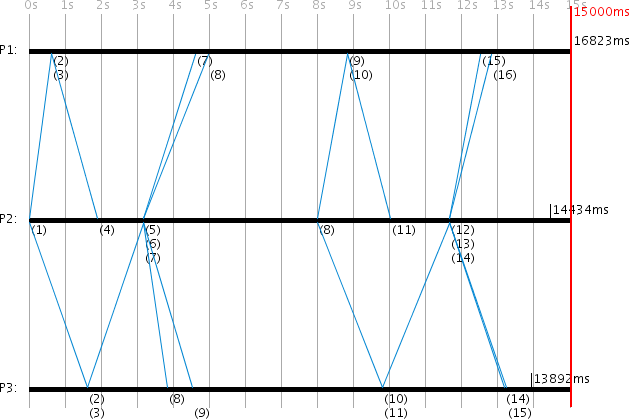
\includegraphics[width=10cm]{images/ss-protokoll-berkeley-lamport}}
	\caption{Lamport-Zeitstempel}
	\label{fig:Lamportzeit}
\end{figure}

Die Vektor- und Lamport-Zeitstempel lassen sich sehr gut am bereits behandeltem Beispiel des Berkeley-Protokoll's (vgl. Kap. 3.6.) demonstrieren. Nach Aktivierung des Lamportzeit-Schalters erscheint bei jedem Ereignis eines Prozesses der aktuelle Lamport-Zeitstempel (s. Abb. \ref{fig:Lamportzeit}.). Jeder Prozess besitzt einen eigenen Lamport-Zeitstempel, der beim Versenden und Erhalten einer Nachricht inkrementiert wird. Jeder Nachricht wird die aktuelle Lamportzeit $t_l(i)$ des Senderprozesses $i$ beigef�gt. Wenn ein weiterer Prozess $j$ diese Nachricht erh�lt, so wird der aktuelle Lamport-Zeitstempel $t_l(j)$ von Prozess $j$ wie folgt neu berechnet:

\begin{equation*}
	t_l(j) := 1 + max(t_l(j), t_l(i))
\end{equation*}

Es wird also stets die gr��ere Lamportzeit vom Sender- und Empf�ngerprozess verwendet und anschlie�end um \textit{1} inkrementiert. Nach Ablauf der Berkeley-Simulation hat P1 \textit{(16)}, P2 (\textit{14}) und P3 (\textit{15}) als Lamport-Zeitstempel abgespeichert. 

\begin{figure}[h]
	\centering
	\fbox{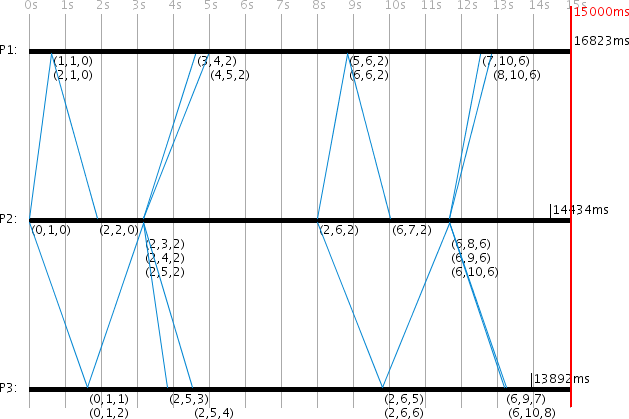
\includegraphics[width=10cm]{images/ss-protokoll-berkeley-vektor}}
	\caption{Vektor-Zeitstempel}
	\label{fig:Vektorzeit}
\end{figure}

Mit aktivem Vektorzeit-Schalter werden alle Vektor-Zeitstempel angezeigt (s. Abb. \ref{fig:Vektorzeit}.). Wie beim Lamport-Zeitstempel wird auch hier jeder Nachricht der aktuelle Vektor-Zeitstempel des Senderprozesses beigef�gt. Bei $n$ beteiligten Prozessen hat der Vektor-Zeitstempel $v$ die Gr��e $n$. Somit gibt es f�r jeden beteiligten Prozess $i$ einen eigenen Index $i$. Mit $v(i)$ kann jeder Prozess auf seinen lokalen Eintrag zugreifen. Wenn $v$ der Vektor-Zeitstempel des Empf�ngerprozesses $j$ ist und $w$ der Vektor-Zeitstempel des Senderprozesses ist, dann wird der neue lokale Vektor-Zeitstempel wie folgt neu berechnet:

\textbf{Pseudo-Code}

\begin{code}
for (i := 0; i < n; i++) {
    if (i = j) {
        v(i)++;
    } else if (v(i) < w(i)) {
        v(i) := w(i);
    }
}
\end{code}

Standardm��ig wird der Vektor-Zeitstempel nur inkrementiert, wenn eine Nachricht verschickt- oder erhalten wird. Bei beiden F�llen inkrementiert der Sender- und Empf�ngerprozess jeweils seinen eigenen Index im Vektor-Zeitstempel um \textit{1}. Beim Empfang einer Nachricht wird anschlie�end der lokale Vektor-Zeitstempel mit dem des Senderprozesses verglichen und f�r alle Indizes stets der gr��ere Wert in den lokalen Vektor-Zeitstempel �bernommen.

Im Beispiel (vgl. Abbildung \ref{fig:Vektorzeit}.) hat P1 \textit{(8,10,6)}, P2 \textit{(6,10,6)}. und P3 \textit{(6,10,8)} als Vektor-Zeitstempel abgespeichert.

Wenn w�hrend einer Simulation Prozesse entfernt- oder neue Prozesse hinzugef�gt werden, so passt sich die Gr��e der Vektor-Zeitstempel aller anderen Prozesse automatisch der Gesamtzahl der Prozesse an.

Wie bereits beschrieben gibt es in den Simulationseinstellungen die boolschen Variablen ``Lamportzeiten betreffen alle Ereignisse'' und ``Vektorzeiten betreffen alle Ereignisse'', die standardm��ig auf \textit{false} gesetzt sind. Mit \textit{true} werden alle Ereignisse, und nicht nur der Empfang oder das Versenden einer Nachricht, ber�cksichtigt. F�r eine weitere Betrachtung der Lamport- sowie Vektor-Zeitstempel siehe \cite{Vorlesung} oder \cite{Tanenbaum}.

\subsection{Simulation langsamer Verbindungen \small{\textit{(slow-connection.dat)}}}

Mit dem Simulator lassen sich auch langsame Verbindungen zu einem bestimmten Prozess simulieren. F�r die Demonstration wird das Beispiel aus Kapitel 3.5. wieder aufgegriffen, wo das Protokoll zur internen Synchronisation (durch P1) mit der Christians-Methode (durch P3) parallel simuliert wurden. P2 stellt den Server beider Protokolle zur Verf�gung. In diesem Szenario soll P3 eine schlechte Netzwerkverbindung besitzen, so dass Nachrichten von- und an P3 stets eine l�ngere �bertragungszeit ben�tigen.

Die Ereignisse sind so wie bereits in Tabelle \ref{tb:InterneSync2Tasks}. dargestellt wurde programmiert. In den Simulationseinstellungen ist hier die Einstellung ``Mittelwerte der �bertragungszeiten bilden'' aktiviert. In den Prozesseinstellungen von P3 wurde die ``Minimale �bertragungszeit'' auf \textit{2000ms} und die ``Maximale �bertragungszeit'' auf \textit{8000ms} gestellt. P1 und P2 behalten als Standardeinstellungen f�r die minimale und maximale �bertragungszeiten die Werte \textit{500ms} und \textit{2000ms}, die Simulationsdauer betr\"{a}gt nun \textit{20000ms}.

\begin{figure}[h]
	\centering
	\fbox{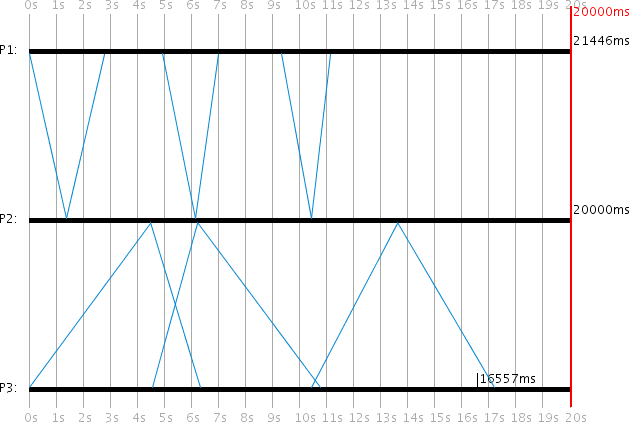
\includegraphics[width=10cm]{images/ss-protokoll-time-sync-2-long-transfer}}
	\caption{Simulation einer langsamen Verbindung}
	\label{fig:TimeSync2LongTransferProto}
\end{figure}

Als Folge (s. Abb. \ref{fig:TimeSync2LongTransferProto}.) ben�tigen Nachrichten, die von- und an P3 verschickt werden, f�r eine �bertragung immer mehr Zeit. Bevor P3 eine Antwort auf seine vorherige Anfrage bekommt, verschickt er eine erneute Anfrage. Da P3 die Serverantworten immer stets seiner letzten verschickten Anfrage zuordnet, berechnet er alle RTTs inkorrekt und seine lokale Zeit wird dadurch bei jedem Durchgang erneut falsch bestimmt. Die Berechnungsformeln der �bertragungszeiten wurde bereits in Kapitel 2.4.3. bei den Prozesseinstellungen behandelt. Konkret bedeutet dies hier f�r die �bertragungszeiten alle Nachrichten von- und an P3 jeweils:

\begin{equation*}
	\frac{1}{2} (rand(500, 2000) + rand(2000, 8000)) = \frac{1}{2} rand(2500, 10000) = rand(1250, 5000) ms
\end{equation*}

In dem Beispiel in Abbildung \ref{fig:TimeSync2LongTransferProto}. ist die lokale Prozesszeit von P1 bis auf \textit{20000 - 21446 = - 1446ms} synchronisiert, w\"{a}hrend die Prozesszeit von P3 ganze \textit{20000 - 16557 = 3443ms} falsch geht.

\chapter{Die Implementierung}

In diesem Kapitel wird auf die Implementierung des Simulators eingegangen. Der Simulator wurde in der Programmiersprache Java entwickelt. Bei der Betrachtung der Zielgruppe wird klar, dass Java f\"{u}r die gestellte Aufgabe die geigneste Programmiersprache ist. Der Simulator ist somit auf jeder Platform verf\"{u}gbar, f\"{u}r die es die JRE (Java Runtime Environment) gibt und erstreckt sich somit \"{u}ber alle g\"{a}ngigen Betriebssysteme. Da an der Fachhochschule Aachen auch Java gelehrt wird, sollten hier die meisten Studenten auch eigene Erweiterungen, wie eigene Protokolle, entwerfen k\"{o}nnen. Der Simulator wurde mit dem derzeit aktuellsten Java SDK (Software Development Kit) in der Version 6 (1.6) entwickelt.

\begin{table}
	\fbox{
	\begin{tabular}{l|l}
		\textbf{Paketname} & \textbf{Beschreibung} \\
		\hline 
		\textit{core} & Klassen f\"{u}r Prozesse und Nachrichten\\
		\textit{core.time} & Klassen f\"{u}r Zeitformate\\
		\textit{events} & Basisklassen f\"{u}r Ereignisse\\
		\textit{events.implementations} & Implementierungen von Ereignissen\\
		\textit{events.internal} & Implementierungen von internen Ereignissen\\
		\textit{exceptions} & Klassen f\"{u}r Fehlerbehandlungen\\
		\textit{prefs} & Klassen f\"{u}r die Einstellungen\\
		\textit{prefs.editors} & Klassen f\"{u}r die Editoren\\
		\textit{protocols} & Basisklassen f\"{u}r Protokolle\\
		\textit{protocols.implementations} & Implementierungen von Protokollen\\
		\textit{serialize} & Helferklassen f\"{u}r die Serialisierung von Simulationen\\
		\textit{simulator} & Klassen f\"{u}r die GUI und die Visualisierung\\
		\textit{utils} & Diverse Helferklassen\\
	\end{tabular}
	}
	\caption{Die Paketstruktur}
	\label{tb:Pakete}
\end{table}

Da es sonst den Rahmen sprengen w\"{u}rde, soll im Folgenden der komplette Quelltext nicht bis in das letzte Detail behandelt werden. Der Quelltext erstreckt sich n\"{a}mlich, einschlie�lich Kommentare, auf \"{u}ber 15.000 Zeilen und \"{u}ber 59 Dateien. Zudem ist die generierte Quelltext-Dokumentation (Javadoc) \"{u}ber 2MB gro�. Alle folgenden UML-Diagramme stellen aufgrund der \"{U}bersichtlichkeit lediglich die wesentlichen Dinge dar. Alle Details lassen sich im Quelltext und der dazugeh\"{o}rigen Dokumentation einsehen. Die Paketstruktur des Quelltextes ist in Tabelle \ref{tb:Pakete} in alphanumerischer Reihenfolge aufgef\"{u}hrt.  

\section{Programmierrichtlinien}

Die Programmierrichtlinien entsprechen in den meisten F\"{a}llen denen aus der Vorlesung \cite{OOS}. Die Main-Methode befindet sich in der Klasse \textit{simulator.VSMain}. 

\begin{itemize}
	\item Alle Klassen- und Interfacenamen beginnen mit gro�en Buchstaben, w\"{a}hrend alle Variablen-, Methoden- und Attributnamen mit kleinen Buchstaben beginnen. Namen statischer Variablen und Attribute sind komplett in Gro�buchstaben gehalten.
	\item Alle Quelltext-Dateien besitzen einen Header, der Informationen der verwendeten Lizenz angibt.
	\item Alle Quelltext-Dateien sind vollst\"{a}ndig mit Javadoc dokumentiert worden. 
	\item Der komplette Quelltext inklusive Dokumentation wurde in englischer Sprache verfasst. 
	\item Eine Quelltext-Datei hat eine maximale Zeilenl\"{a}nge von 80 Zeichen. Eine Ausnahme stellt die Klasse \textit{prefs.VSDefaultPrefs} dar, denn hier befinden sich auch l\"{a}ngere Texte die in Strings abgespeichert werden, wo manuelle Zeilenumbr\"{u}che wenig Sinn ergeben. 
	\item Es werden zuerst Klassen aus der Java-Standardbibliothek importiert, bevor Klassen aus dem VS-Simulator selbst importiert werden.
	\item F\"{u}r die Einr\"{u}ckung des Quelltextes wird das Tool \textit{astyle} mit den Aufrufparametern \textit{--style=java --mode=java} verwendet. Hierbei wird eine Einr\"{u}ckungsl\"{a}nge von 4 Zeichen verwendet.
	\item Namen abstrakter Klassen tragen stets das Prefix \textit{VSAbstract}.
	\item Namen aller Klassen und Interfaces tragen als Prefix stets \textit{VS}, was f\"{u}r Verteilte Systeme steht. 
	\item Namen aller Protokollklassen tragen als Postfix \textit{Protocol}, zum Beispiel \textit{VSPingPongProtocol}.
	\item \"{U}berall wo es Sinn ergibt werden Java-Generic-Datentypen verwendet (z.B. \textit{java.util.Vector<Integer>} anstelle von \textit{java.util.Vector}.
\end{itemize}



\section{Einstellungen und Editoren}

Eine Simulation ist von einer Vielzahl von Einstellungen abh\"{a}ngig. Da auf diese Einstellungen in den weiteren Teilkapitel sets zur\"{u}ckgegriffen wird, macht es Sinn die dazugeh\"{o}rigen Klassen zuerst zu betrachten.

\subsection{Einstellungsobjekte}

Auf Abbilung \ref{fig:PackagePrefs} ist der Aufbau des Pakets \textit{prefs} zu sehen. In einer Instanz der Klasse \textit{VSPrefs} lassen sich viele verschiedene Daten als Variablen f\"{u}r eine sp\"{a}tere Verwendung dynamisch ablegen und stellt somit einen Container f\"{u}r diese Daten dar. In einem \textit{VSPrefs}-Objekt speichert der Simulator alle seine Einstellungen ab. Zudem besitzt jedes Prozessobjekt und jedes Ereignisobjekt (und da Protokolle auch Ereignisse sind auch jedes Protokollobjekt) f\"{u}r lokale Einstellungen seine eigene Instanz von \textit{VSPrefs}. Selbst Nachrichtenobjekte besitzt hiervon eine eigene Instanz, wobei hier die zu verschickenden Daten abgelegt werden k\"{o}nnen.

\begin{figure}[h]
	\centering
	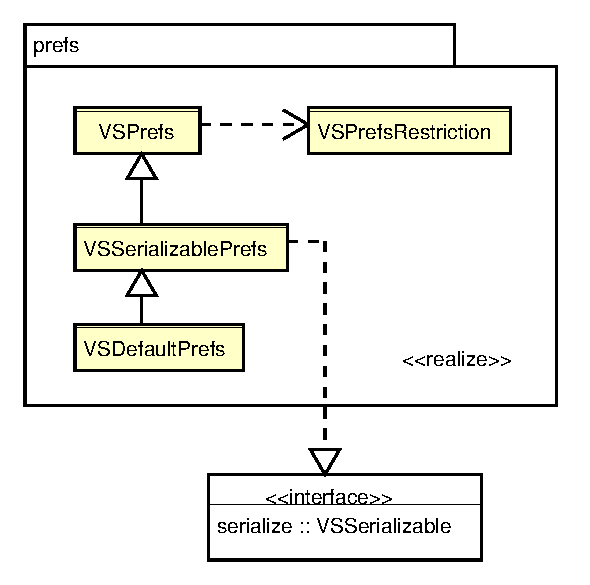
\includegraphics[width=7cm]{images/prefs}
	\caption{Das Paket \textit{prefs}}
	\label{fig:PackagePrefs}
\end{figure}

Jede Variable besteht aus einen Datentypen, einen Variablenamen und einer optionalen Beschreibung sowie einen Wert. Einige Datentypen unterst\"{u}tzen auch die Angabe von Minimum- und Maximumwerten (zum Beispiel besteht eine Prozentangabe aus einen Integerwert zwischen \textit{0} und \textit{100}), was mithilfe der \textit{VSPrefsRestriction}-Klasse implementiert wird. Da man beispielsweise bei Prozent ein \textit{\%} und bei Millisekunden ein \textit{ms} hinter der Variable sehen m\"{o}chte, kann f\"{u}r jede Variable auch ein optionaler Einheiten-String abgespeichert werden. 

Eine Variablenbeschreibung wird f\"{u}r die Darstellung im GUI verwendet, w\"{a}hrend der Variablenname eher f\"{u}r die interne Verwendung vom Simulator verwendet wird. Zum Beispiel hat die Variable \textit{message.prob.outage} (Verlustwahrscheinlichkeit einer Nachricht) die Variablenbeschreibung ``Nachrichtenverlustw'keit''. Wenn f\"{u}r eine Variable keine Beschreibung existiert so wird, wie auf Abbildung \ref{fig:SimulationseinstellungenExperten} anhand der Farbvariablen schon gesehen wurde, f\"{u}r die Anzeige f\"{u}r eine Variable der Datentyp und der Variablenname verwendet. Variablennamen verwenden die auf Tabelle \ref{tb:VariablenPrefixe} angegebenen Prefixe. Alle verf\"{u}gbaren Typen wurden bereits in Tabelle \ref{tb:VariablenDatentypen} aufgelistet. \textit{VSPrefs} stellt f\"{u}r alle Variablen entsprechende Zugriffsmethoden zur Verf\"{u}gung.  

Im Folgenden werden nicht alle exisierenden Methoden aufgelistet, da diese auch in der Quelltext-Dokumentation (Javadoc) eingesehen werden k\"{o}nnen. Die Methoden werden nun nur anhand des Integer-Datentyps verdeutlicht. F\"{u}r alle anderen Typen gilt fast alles analog. F\"{u}r Integer stehen in \textit{VSPrefs} folgende Methoden zur Verf\"{u}gung:

\begin{itemize}
	\setlength{\itemsep}{-2mm}
	\item \textit{void setInteger(String key, Integer val)}
	\item \textit{void setInteger(String key, Integer val, String descr)}
	\item \textit{void setInteger(String key, int val)}
	\item \textit{void setInteger(String key, int val, String descr)}
	\item \textit{Integer getIntegerObj(String key)}
	\item \textit{int getInteger(String key)}
	\item \textit{java.util.Set<String> getIntegerKeySet()}
	\item \textit{void initInteger(String key, int val) }
	\item \textit{void initInteger(String key, int val, String descr) }
	\item \textit{void initInteger(String key, int val, String descr, int minValue, int maxValue) }
	\item \textit{void initInteger(String key, int val, String descr, int minValue, int maxValue, String unit) }
	\item \textit{void initInteger(String key, int val, String descr, VSPrefsRestriction.VSIntegerPrefsRestriction r) }
	\item \textit{void initInteger(String key, int val, String descr, VSPrefsRestriction.VSIntegerPrefsRestriction r, String unit) }
\end{itemize}

\begin{table}
	\fbox{
	\begin{tabular}{c|l|l}
		\textbf{Variablen-Prefix} & \textbf{Beschreibung}  & \textbf{Beispiel}\\
		\hline 
		\textit{col} & Farbvariablen & \textit{Color: col.background = Color-Objekt}\\
		\textit{div} & Diverse versteckte Variablen & \textit{Integer: div.window.loggsize = 300} \\
		\textit{keyevent} & Variablen, die Tastaturk\"{u}rzel definieren & \textit{Integer: keyevent.close = KeyEvent.VK\_C} \\
		\textit{lang} & Variablen, die Text beinhalten & \textit{String: lang.activate = aktivieren}\\
		\textit{message} & Variablen, die Nachrichten betreffen & \textit{Integer: message.prob.outage = 0}\\
		\textit{process} & Variablen, die Prozesse betreffen & \textit{Integer: process.prob.crash = 0}\\
		\textit{sim} & Allgemeine Simulationsvariablen & \textit{Integer: sim.process.num = 3}\\
	\end{tabular}
	}
	\caption{Konventionen f\"{u}r Variablennamen-Prefixe in \textit{VSDefautPrefs}}
	\label{tb:VariablenPrefixe}
\end{table}

Hierbei stellt \textit{key} den Variablennamen- und \textit{val} den Variablenwert dar. \textit{descr} ist eine optionale Variablenbeschreibung. Es k\"{o}nnen sowohl Java's Integer-Objekte, als auch Java's primitiver Integer-Typ \textit{int} verwendet werden. Ein \textit{int}-Wert wird intern allerdings als Integer-Objekt abgespeichert und macht somit keinen gro�en Unterschied. Die Methode \textit{getIntegerKeySet} gibt alle vorhandenen Integer-Variablennamen (\textit{key}s) als \textit{Set} zur\"{u}ck.

\textit{VSPrefs} bietet auch eine Reihe von \textit{initInteger}-Methoden an, welche sich von den \textit{setInteger}-Methoden dadurch unterscheiden, dass sie eine Variable nur einen Wert zuweisen, wenn sie vorher noch nicht initialisiert wurde, was durch \textit{setInteger} oder \textit{initInteger} selbst geschehen sein kann. Eine komplette \"{U}bersicht aller Methoden (auch f\"{u}r andere Datentypen) gibt es in der Quelltext-Dokumentation.

\textit{VSPrefs} speichert alle Integervariablen in einem \textit{HashMap<String,Integer>}-Objekt ab, wobei der String-Wert den Variablenamen \textit{key} angibt. F\"{u}r die Beschreibung \textit{descr}, den Einheiten-String \textit{unit} sowie m\"{o}glichen Minimum- und Maximumwerte werden separate Instanzen von \textit{HashMap} verwendet. Da alle \textit{HashMap}-Objekte synchronisiert sind, k\"{o}nnen alle Methoden von verschiednenen Threads gleichzeitig verwendet werden. 

Die Klasse \textit{VSDefaultPrefs} erweitert \textit{VSPrefs} und initialisiert bei Instanzierung automatisch alle verf\"{u}gbaren Simulationsvariablen mit ihren Standardwerten. Dort sind auch alle Spracheinstellungen abgelegt. Sollte jemand den Simulator in eine andere Sprache, zum Beispiel ins Englische, \"{u}bersetzen wollen, so mu� er lediglich diese Datei und die Protokoll-Klassen (mehr dazu sp\"{a}ter) editieren. Die Spracheinstellungen sind n\"{a}mlich in einem \textit{VSPrefs}--Objekt als versteckte String-Variablen abgespeichert. Spracheinstellungen f\"{u}r Protokolle wurden in den Protokollklassen direkt angegeben, da dies mehr Komfort f\"{u}r den Protokollentwickler bietet und f\"{u}r jede neue Textausgabe nicht st\"{a}ndig \textit{VSDefaultPrefs.java} editiert werden muss. 

Alle Variablen die als Prefix \textit{lang}, \textit{keyevent}, \textit{div} oder \textit{col} tragen, sind versteckte Variablen und werden in einem Editor nicht angezeigt. Im Expertenmodus sind hingegen nur Variablen die mit \textit{lang} und \textit{keyevent} beginnen versteckt. Somit lassen sich im Expertenmodus weitere Variablen vom Anwender editieren.

\subsection{Editorobjekte}

\begin{figure}[h]
	\centering
	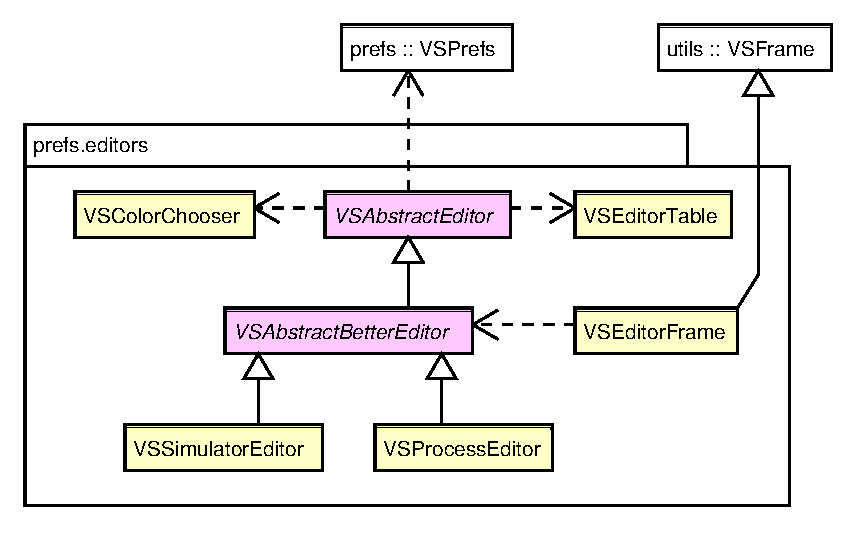
\includegraphics[width=11cm]{images/prefs-editors}
	\caption{Das Paket \textit{prefs.editors}}
	\label{fig:PackagePrefsEditors}
\end{figure}

Wie Variablen intern abgespeichert werden ist bereits bekannt. F\"{u}r das Editieren der Variablen werden Editor-Objekte verwendet. Auf Abbildung \ref{fig:PackagePrefsEditors} ist die Klassenstruktur des dazugeh\"{o}rigen Paketes \textit{prefs.editors} angegeben. 

Die Basis eines Editors stellt die abstrakte Klasse \textit{VSAbstractEditor} dar, dem ein \textit{VSPrefs} Objekt zum Editieren \"{u}bergeben wird. Ein Editor stellt alle verf\"{u}gbaren und nicht-versteckten Variablen des \textit{VSPrefs}-Objektes im GUI dar und bietet gleichzeitig die M\"{o}glichkeit alle Variablen dar\"{u}ber zu editieren an. F\"{u}r das Editieren von Farbwerten wird auf \textit{VSColorChooser} zur\"{u}ckgegriffen. Die Klasse \textit{VSEditorTable} ist f\"{u}r das \textit{JTable}-Objekt aus Java's Swing-Bibliothek zust\"{a}ndig, welches bei der graphischen Darstellung aller Variablen eingesetzt wird. Die abstrakte Klasse \textit{VSAbstractBetterEditor} wurde, wegen der \"{U}bersicht, als Zwischenschritt eingef\"{u}gt. 

Die Klasse \textit{VSSimulatorEditor} dient f\"{u}r das Editieren der globalen Simulationseinstellungen und \textit{VSProcessEditor} f\"{u}r das Editieren der Prozesseinstellungen sowie der dazugeh\"{o}rigen Protokollvariablen. Da diese beiden Klassen von \textit{VSAbstractBetterEditor} erben, k\"{o}nnen sie mithilfe von \textit{VSEditorFrame} in einem separaten Fenster angezeigt werden. Alternativ k\"{o}nnen die Editoren auch in der Sidebar im Tab ``Variablen'' angezeigt werden. Auf Abbildung \ref{fig:Simulationseinstellungen} wurde bereits ein \textit{VSEditorFrame} in Aktion gesehen.

F\"{u}r Protokolle gibt es keine separate Editor-Klasse, da sie bereits vom Prozesseditor aus editiert werden k\"{o}nnen. Dabei iteriert der Prozesseditor \"{u}ber alle f\"{u}r den jeweiligen Prozess verf\"{u}gbaren Protokollobjekte und f\"{u}gt deren Variablen zus\"{a}tzlich in den Prozesseditor ein. Somit erscheinen die Prozess- und die dazugeh\"{o}rigen Protokollvariablen im selben Editor, womit dem Benutzer eine bessere \"{U}bersicht geboten wird. 

\section{Ereignisse}

\subsection{Funktionsweise von Ereignissen}

F\"{u}r jedes Ereignis existiert eine dazugeh\"{o}rige Klasse, welche die auszuf\"{u}hrenden Aktionen implementiert. Eine Instanz davon wird, f\"{u}r eine sp\"{a}tere Ausf\"{u}hrung, in einem \textit{VSTask}-Objekt verpackt dem Task-Manager \"{u}bergeben. Auf den Task-Manager wird sp\"{a}ter noch genauer eingegangen. 
\begin{figure}[h]
	\centering
	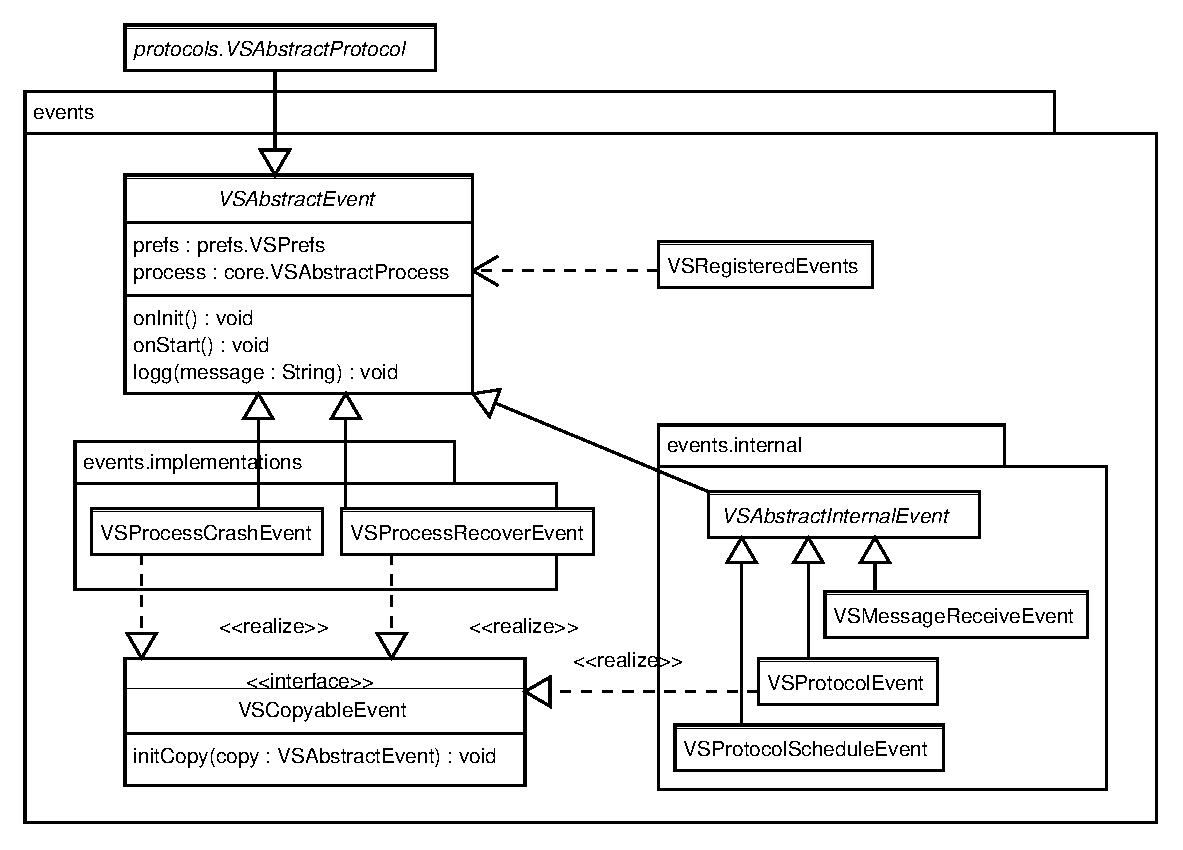
\includegraphics[width=13.5cm]{images/events}
	\caption{Die Pakete \textit{events} und \textit{events.*}}
	\label{fig:PackageEvents}
\end{figure}

Jedes programmierbare Ereignis mu�, bevor es vom Simulator verwendet werden kann, in der statischen Klasse \textit{VSRegisteredEvents} registriert werden. Da sich die Anzahl der verf\"{u}gbaren Ereignisse bei Laufzeit des Simulators nicht \"{a}ndert, gibt es keine Instanzen von \textit{VSRegisteredEvents}. Alle Methoden und Klassenattribute sind hier statisch. Wenn beispielsweise eigene Ereignisse implementiert werden, dann m\"{u}ssen alle neuen Ereignisse per Hand in die Datei \textit{VSRegisteredEvents.java} \"{u}bernommen- und der Simulator erneut kompiliert werden.

In der Implementierung wird zwischen drei Haupttypen von Ereignissen unterschieden, die jeweils in verschiedenen Paketen liegen (siehe auch die leicht vereinfachte Abbildung \ref{fig:PackageEvents}):

\begin{enumerate}
	\item \textit{events.implementations}: In diesem Paket befinden sich alle Ereignisse, die ohne weitere Spezialbehanldung im Simulator eingesetzt werden k\"{o}nnen und vom Benutzer direkt im Ereigniseditor programmierbar sind. 
		\begin{itemize}
			\item \textit{VSProcessCrashEvent}: Dieses Ereignis l\"{a}sst den dazugeh\"{o}rigen Prozess abst\"{u}rzen.
			\item \textit{VSProcessRecoverEvent}: Dieses Ereignis l\"{a}sst den dazugeh\"{o}rigen Prozess wiederbeleben.
		\end{itemize}

	\item \textit{events.internal}: In diesem Paket befinden sich alle Ereignisse, die vom Simulator intern verwendet werden und dadurch eine direkte Programmierung via Ereigniseditor ausschlie�en. 		
		\begin{itemize}
			\item \textit{VSAbstractInternalEvent}: Diese Klasse stellt weitere Methoden zur Verf\"{u}gung, die von allen internen Ereignissen ben\"{o}tigt werden. Derzeit betrifft dies nur Methoden zur Serialisierung der gegebenen Objekte. Auf die Serialisierung (Abspeichern/Laden) von Simulationen wird sp\"{a}ter noch genauer eingegangen.
			\item \textit{VSMessageReceiveEvent}: Diese Klasse wird f\"{u}r die Ankunft einer Nachricht bei einem Empf\"{a}ngerprozess ben\"{o}tigt. Sie kapselt die eigentliche Nachricht und \"{u}berpr\"{u}ft, ob der Empf\"{a}ngerprozess das zur Nachricht dazugeh\"{o}rige Protokoll versteht. Diese Klasse \"{u}berpr\"{u}ft auch die Simulationseinstellung ``Nur relevante Nachrichten anzeigen'' und entscheidet, ob die Nachricht nach Eintreffen in der Visualisierung und im Loggfenster ber\"{u}cksichtigt werden soll oder nicht.
			\item \textit{VSProtocolEvent}: Diese Klasse implementiert gleichzeitig vier verschiedene Ereignisse: Das Aktivieren/Deaktivieren eines Servers/Clients eines gegebenen Protokolls. Der Ereigniseditor berechnet anhand der verf\"{u}gbaren Protokolle automatisch alle m\"{o}glichen Kombinationen und bietet sie dem Anwender in seiner Auswahl an. F\"{u}r alle dieser vier Ereignisse wird jeweils ein Objekt von \textit{VSProtocolEvent} verwendet, jedoch mit jeweils anderen Attributwerten.  
			\item \textit{VSProtocolScheduleEvent}: Diese Klasse wird f\"{u}r die Wecker-Ereignisse ben\"{o}tigt. Wecker-Ereignisse k\"{o}nnen nur von Protokollen (mehr dazu sp\"{a}ter) erstellt werden. \textit{VSProtocolScheduleEvent} besitzt eine Referenz auf das gegebene Protokoll und ruft bei Ereigniseintrittszeit entweder die Methode \textit{onServerScheduleStart} bei einem Server- oder \textit{onClientScheduleStart} bei einem Clientprotokoll auf. 
		\end{itemize}
	\item \textit{protocols.implementations}: In diesem Paket befinden sich alle Protokollimplementierung. Jedes Protokoll besitzt hier seine eigene Klasse. Alle Protokolle erben hierbei von der auf Abbildung \ref{fig:PackageEvents} zu sehenden Klasse \textit{protocols.VSAbstractProtocol}. Da \textit{protocols.VSAbstractProtocol} von \textit{events.VSAbstractEvent} erbt, kann ein Protokollobjekt auch als Ereignis eingesetzt werden. Ein solches Ereignis ruft bei Eintritt entweder die Methode \textit{onServerStart} oder die Methode \textit{onClientStart} des Protokolls auf, was einer Server- beziehungsweise einer Clientanfrage entspricht. Die Implementierung von Protokollen wird sp\"{a}ter genauer behandelt. 
\end{enumerate}

Alle Ereignisse, die das Interface \textit{VSCopyableEvent} implementieren, k\"{o}nnen vom Anwender im Ereigniseditor mit einem Rechtsklick kopiert werden und m\"{u}ssen die Methode \textit{initCopy(VSAbstractEvent copy)} implementieren. Dort werden alle relevanten Attribute in das neue Ereignis \textit{copy} kopiert. 

Alle Ereignisklassen erweitern die abstrakte Klasse \textit{VSAbstractEvent} und m\"{u}ssen folgende abstrakten Methoden implementieren:

\begin{itemize}
	\item \textit{abstract public void onInit()}: Bevor ein Ereignisobjekt vom Simulator verwendet werden kann, mu� es initialisiert werden. Je nach Ereignis k\"{o}nnen hier verschiedene Werte initialisiert werden. Diese Methode wird pro Ereignisobjekt nach Erstellung nur ein einziges Mal ausgef\"{u}hrt. 
	\item \textit{abstract public void onStart()}: Diese Methode wird jedes Mal ausgef\"{u}hrt, wenn das Ereignis eintritt. Sie stellt somit das Kernst\"{u}ck eines Ereignisses dar. 
\end{itemize}

Des Weiteren werden folgende nicht-abstrakte Methoden von \textit{VSAbstractEvent} vererbt:

\begin{itemize}
	\item \textit{public void logg(String message)}: Diese Methode schreibt eine Loggnachricht in das Simulationsloggfenster.
	\item \textit{public VSAbstractEvent getCopy()}: Diese Methode erstellt vom aktuellen Ereignis eine Kopie, wovon eine Referenz zur\"{u}ckgegeben wird. Alle Ereignisse die kopiert werden k\"{o}nnen m\"{u}ssen ebenso das Interface \textit{VSCopyableEvent} implementieren. Wenn ein Ereignis dies nicht tut und \textit{getCopy()} aufgerufen wird, dann wird von Java die Ausnahme \textit{exceptions.VSEventNotCopyable} geworfen.
	\item \textit{public VSAbstractEvent getCopy(VSInternalProcess process)}: Diese Methode erstellt vom aktuellen Ereignis ebenfalls eine Kopie, jedoch mit dem Unterschied, dass das Ereignis einem anderen Prozess zugewiesen wird. 
\end{itemize}

Jede Ereiginsklasse hat zudem Zugriff auf folgende Attribute, die von \textit{VSAbstractEvent} vererbt werden:

\begin{itemize}
	\item \textit{protected VSPrefs prefs}: Eine Referenz auf das Simulationseinstellungsobjekt. Hier\"{u}ber lassen sich alle Simulationseinstellungen beziehen. \textit{prefs} ist nicht zu verwechseln mit den TODO 
	\item \textit{protected VSAbstractProcess process}: Eine Referenz auf das Prozessobjekt des jeweiligen Prozesses, auf welches das Ereignis angewendet wird.
\end{itemize}

\subsection{Beispielimplementierung eines Ereignisses}

Im Folgenden wird als Beispiel die Implementierung des Prozessabsturzereignisses \textit{VSProcessCrashEvent} behandelt. Da die dazugeh\"{o}rige Klasse keine Attribute besitzt, verleibt hier auch die \textit{initCopy}-Methode mit leerem Rumpf. Jede Ereignisklasse muss in \textit{onInit()} mit \textit{setClassname} den eigenen Klassennamen mitteilen. In \textit{onStart()} wird das eigentliche Ereignis ausgef\"{u}hrt. Hier wird obligatorisch \"{u}berpr\"{u}ft, ob der Prozess bereits abgest\"{u}rzt (hier eigentlich nicht Notwendig, verbessert aber die Lesbarkeit der Logik) ist und gegebenenfalls wird der Prozess dann zum Absturz bewegt. Der Task-Manager \"{u}berpr\"{u}ft bereits, ob der Prozess abgest\"{u}rzt ist oder nicht, d.h. ein Ereignis wird bei einem abgest\"{u}rztem Prozess gar nicht erst ausgef\"{u}hrt. Die einzige Ausnahme bildet ein Wiederbelebungsereignis (\text{VSProcessRecover}), welches vom Task-Manager ausgef\"{u}hrt wird, auch wenn der Prozess abgest\"{u}rzt ist. Mit \textit{logg} wird eine Nachricht in das Loggfenster geschrieben, welche ueber das \textit{VSPrefs}-Objekt \textit{prefs} bezogen wird:
\begin{code}
package events.implementations;

import events.*;

public class VSProcessCrashEvent 
extends VSAbstractEvent implements VSCopyableEvent {
    public void initCopy(VSAbstractEvent copy) {
    }

    public void onInit() {
        setClassname(getClass().toString());
    }

    public void onStart() {
        if (!process.isCrashed()) {
            process.isCrashed(true);
            logg(prefs.getString("lang.crashed"));
        }
    }
}
\end{code}

\section{Zeitformate, Prozesse, Nachrichten sowie Task-Manager}

\subsection{Funktionsweise}

Das Paket \textit{core.time} auf Abbildung \ref{fig:PackageCoreTime} stellt lediglich die Klassen f\"{u}r die Vektor- und Lamportzeitstempel zur Verf\"{u}gung. F\"{u}r die normale lokale Prozesszeit wird aus Performancegr\"{u}nden keine eigene Klasse, sondern ein einfaches \textit{long}-Attribut des Prozessobjektes verwendet.

\begin{figure}[h]
	\centering
	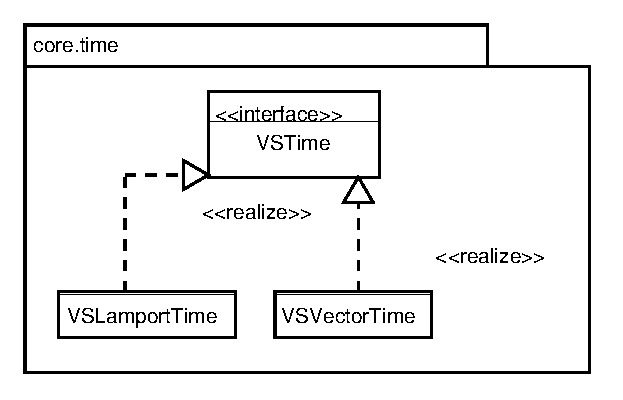
\includegraphics[width=7cm]{images/core-time}
	\caption{Das Paket \textit{core.time}}
	\label{fig:PackageCoreTime}
\end{figure}

Auf Abbildung \ref{fig:PackageCore} ist stark vereinfacht (in Wirklichkeit existieren in den angegebenen Klassen viel mehr Attribute und Methoden) das Paket \textit{core} dargestellt. F\"{u}r jedes auszuf\"{u}hrendes Ereignis wird eine Instanz von \textit{VSTask} ben\"{o}tigt, welche die Ereigniseintrittszeit als Attribut abgespeichert hat sowie eine Referenz auf das Objekt des auszuf\"{u}hrenden Ereignisses (\textit{VSAbstractEvent}) und dem Prozessobjekt besitzt. Geplante \textit{VSTask}-Instanzen werden f\"{u}r eine sp\"{a}tere Ausf\"{u}hrung dem Task-Manager \"{u}bergeben.

Die Kapselung eines \textit{VSAbstractEvent}-Objektes in einem \textit{VSTask}-Objekt erlaubt es, dass die selbe \textit{VSAbstractEvent}-Instanz mehrmals auf einmal im Task-Manager geplant werden kann. Ohne dieser Kapselung g\"{a}be es f\"{u}r jedes Ereignis lediglich nur eine einzige m\"{o}gliche Eintrittszeit. Von dieser M\"{o}glichkeit wird zum Beispiel bei den Server- und Clientanfragen eines Protokollobjektes Gebrauch gemacht. F\"{u}r jedes Protokoll kann der Anwender in einer Simulation beliebig viele Anfragen programmieren, wobei f\"{u}r jede Anfrage stets das selbe Protokollobjekt als Ereignis verwendet wird.

Jede Simulation besitzt genau eine Instanz von \textit{VSTaskManager}. Eine Instanz dieser Klasse stellt den Task-Manager dar. Er verwaltet alle \textit{VSTask}-Instanzen und \"{u}berpr\"{u}ft periodisch, ob es auszuf\"{u}hrende Ereignisse gibt. Der Task-Manager unterscheidet zwischen globalen und lokalen Ereignissen. Hierbei werden alle globalen Ereignisse (gekapselt in einem \textit{VSTask}-Objekt) in einer Priorit\"{a}ts-Warteschlange abgelegt. Die Priorit\"{a}ts-Warteschlange stellt hierbei die korrekte Ereigniseintrittsreihenfolge sicher. Da sich die lokalen Zeiten aller beteiligten Prozesse voneinander unterscheiden k\"{o}nnen, muss f\"{u}r jeden Prozess eine separate lokale Priorit\"{a}ts-Warteschlange verwendet werden, auf die jedes Prozessobjekt seine eigene Referenz hat. In den lokalen Warteschlangen sind die geplanten lokalen Ereignisse (auch gekapselt in einem \textit{VSTask}-Objekt) abgelegt. Der Task-Manager greift \"{u}ber eine \textit{java.util.ArrayList} auf alle Prozessobjekte zu und kann somit auch auf alle lokalen Warteschlangen zugreifen und diese verwalten.

\begin{figure}[h]
	\centering
	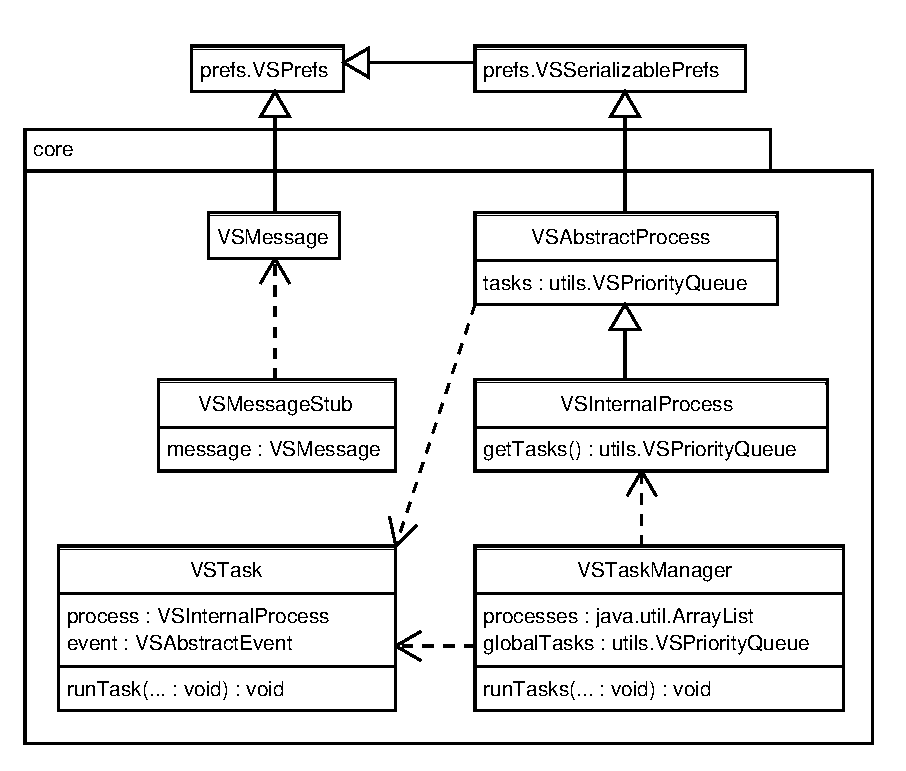
\includegraphics[width=10.0cm]{images/core}
	\caption{Das Paket \textit{core}}
	\label{fig:PackageCore}
\end{figure}

Eine Instanz von \textit{VSMessage} stellt eine Nachricht dar, die von einem Prozess verschickt wird. F\"{u}r jedes Versenden einer Nachricht wird hiervon eine Instanz gebildet, wo der Senderprozess die zu verschickende Daten ablegt. Da \textit{VSMessage} von \textit{VSPrefs} erbt, k\"{o}nnen zwischen zwei Prozessen beliebige Datentypen (Tabelle \ref{tb:VariablenDatentypen}) \"{u}ber eine Nachricht verschickt werden. Anschlie�end wird f\"{u}r jeden Empf\"{a}ngerprozess das neues Ereignisobjekt der Klasse \textit{VSMessageReceiveEvent} angelegt, welche eine Referenz der verschickten Nachricht besitzt. Danach wird ein \textit{VSTask}-Objekt instanziert, wo die Referenz auf das Ereignisobjekt und das dazugeh\"{o}rige Prozessobjekt sowie die Ereigniseintrittszeit als Attribute gespeichert werden. Das \textit{VSTask}-Objekt wird dann dem Task-Manager "{u}bergeben, der das dazugeh\"{o}rige Ereignis ausf\"{u}hrt, wenn die Ereigniseintrittszeit eingetroffen ist. Via Java-Polymorphie wird das \textit{VSMessageReceiveEvent}-Objekt in ein \textit{VSAbstractEvent} umgewandelt. 

Erw\"{a}hnentswert ist auch die Klasse \textit{VSMessageStub}, welche ein \textit{VSMessage} kapselt. Ihr Zweck ist das Verstecken einiger Methoden von \textit{VSMessage} im Protokoll-API, welches f\"{u}r die Erstellung eigener Protokolle dient. Der Protokoll-Entwickler soll m\"{o}glichst nichts falsch machen k\"{o}nnen und deswegen soll den Protokoll-API ein eingeschr\"{a}nkter Funktionsumpfang zur Verf\"{u}rung gestellt werden. Da sich \textit{VSMessageStub} im selben Paket wie \textit{VSMessage} befindet, kann \textit{VSMessageStub} auf paket-private Methoden von \textit{VSMessage} zugreifen. Protokolle hingegen werden in einem anderen Paket implementiert und haben somit keinen Zugriff auf diese paket-privaten Methoden. Zwar kann der Protokollentwickler ein eigenes \textit{VSMessageStub}-Objekt anlegen, jedoch kann er auf diese Weise besser unterscheiden, auf welche Mehhoden er zugreifen sollte und auf welche nicht. Das Protokoll-API wird sp\"{a}ter genauer behandelt. 

Der Task-Manager speichert anschlie�end die Empfangsereignisse in den lokalen Warteschlangen der Empf\"{a}ngerprozesse. Die Nachricht kommt bei einem Empf\"{a}ngerprozess an, sobald das Ereignis f\"{u}r den Empfang eintritt. F\"{u}r die korrekte Implementierung der Lamport- und Vektor-Zeitstempel wird jeder Nachricht automatisch eine Referenz auf die Lamport- sowie auf die Vektorzeit des sendenden Prozesses als Attribut beigef\"{u}gt. F\"{u}r die \"{U}berpr\"{u}fung des Protokolls wird in jeder Nachricht auch der Klassenname des jeweiligen Protokolls abgespeichert.

Eine Instanz von \textit{VSInternalProcess} repr\"{a}sentiert einen simulierten Prozess. Ein \textit{VSInternalProcess} stellt alle vom Simulator intern verwendeten Methoden zur Verf\"{u}gung, w\"{a}hrend ein \textit{VSAbstractProcess} lediglich Methoden hat, die man im Protokoll-API f\"{u}r die Erstellung eigener Protokolle verwenden darf. Da \textit{VSAbstractProcess} abstrakt ist und hiervon keine Instanz gebildet werden darf, muss f\"{u}r einen neuen Prozesses stets ein \textit{VSInternalProcess}-Objekt erstellt werden. Via Polymorphie wird dieses Objekt nach \textit{VSAbstractProcess} umgewandelt und so dem Protokoll-API zur Verf\"{u}gung gestellt. Beispielsweise darf mit \textit{getTasks()} nur vom Simulator intern auf die Priorit\"{a}ts-Warteschlangen zugegriffen werden, w\"{a}hrend man im Protokoll-API selbiges vermeiden sollte und auch gar nicht direkt m\"{o}glich ist. Hierf\"{u}r h\"{a}tte man auch ein Stub-Objekt \textit{VSProcessStub} verwenden k\"{o}nnen. Da aber so gut wie alle paar Millisekunden auf die Methoden von \textit{VSInternalProcess} zugegriffen wird, wurde hier aus Performancegr\"{u}nden der Weg \"{u}ber eine Vererbungungsstufe preferiert. 

Alle einstellbaren Prozessvariablen werden von der Klasse \textit{VSPrefs} vererbt. Damit bei Neuberechnungen die Variablen nicht dauernd \"{u}ber eine \textit{HashMap} von \textit{VSPrefs} zugregriffen werden mu�, speichert \textit{VSInternalProcess} aus Performancegr\"{u}nden einige Variablen als lokale Kopie ab. Zum Beispiel wird f\"{u}r die lokale Prozesszeit nicht auf das \textit{HashMap<String,Long>}-Objekt von \textit{VSPrefs}, sondern auf das Klassenattribut \textit{private long localTime} zugegriffen. Vor- und nach dem Editieren \"{u}ber den Prozesseditor werden die \textit{VSPrefs} beziehungsweise die lokalen Kopien auf den neusten Stand gebracht. Selbiges gilt f\"{u}r weitere Variablen wie zum Beispiel der Uhrabweichung eines Prozesses.

\subsection{Beispiel f\"{u}r die Erstellung von Prozessereignissen}

Anhand der Prozessabsturz- und Wiederbelebungsereignisse l\"{a}�t sich wie folgt sehr gut demonstieren, wie intern Ereignisse angelegt werden k\"{o}nnen:
\begin{code}
void createCrashAndRecoverExample(VSTaskManager taskManager,
                                  VSInternalProcess process) {
    VSAbstractEvent crashEvent = new VSProcessCrashEvent();
    VSTask localTask = new VSTask(process.getTime()+500, process, 
                                  crashEvent, VSTask.LOCAL);
    taksManager.addTask(localTask);

    VSAbstractEvent recoverEvent = new VSProcessRecoverEvent();
    VSTask globalTask = new VSTask(2000, process, 
                                   recoverEvent, VSTask.GLOBAL);
    taksManager.addTask(globalTask);
}
\end{code}

In diesem Beispiel wurden zwei Ereignisse (Absturz- und Wiederbelebung eines gegebenen Prozesses) angelegt. Das Absturzereignis tritt bei der aktuellen lokalen Prozesszeit plus \textit{500ms} ein, w\"{a}hrend das Wiederbelebungsereignis bei einer globalen Zeit von \textit{2000ms} stattfindet. F\"{u}r den Fall, dass das Wiederbelebungsereignis vor dem Absturzereignis eintritt wird es nicht ausgef\"{u}hrt, da der Prozess noch nicht abgest\"{u}rzt ist. 

\section{Protokolle}

\subsection{Funktionsweise des Protokoll-APIs}

\begin{figure}[h]
	\centering
	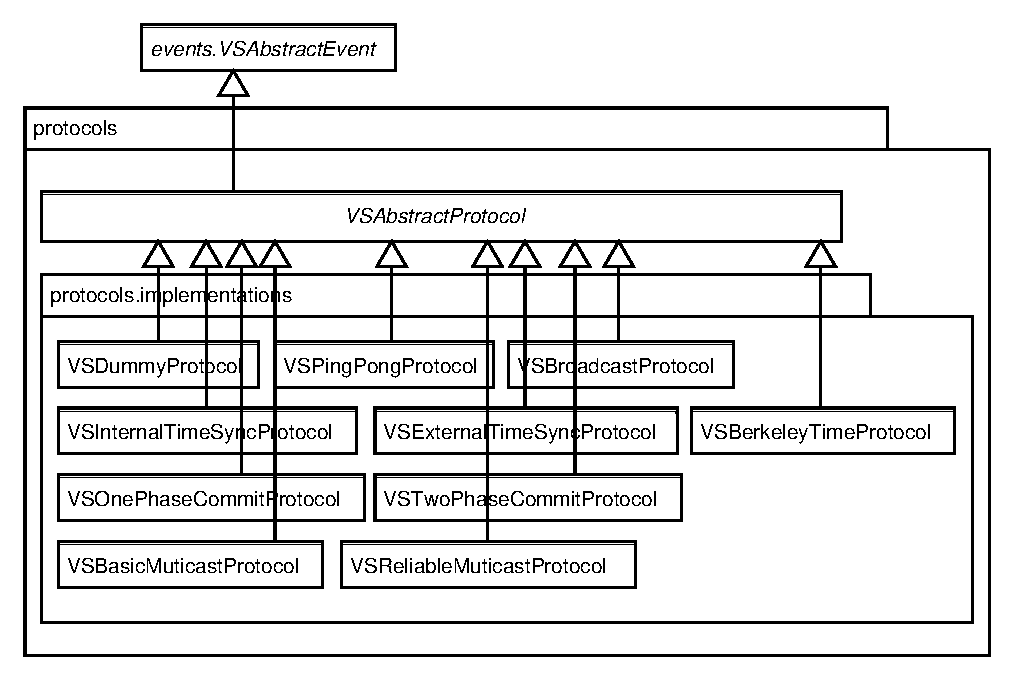
\includegraphics[width=12cm]{images/protocols}
	\caption{Die Pakete \textit{protocols} und \textit{protocols.*}}
	\label{fig:PackageProtocols}
\end{figure}

In diesem Abschnitt wird auf die Implementierung der Protokolle eingegangen. Auf Abbildung \ref{fig:PackageProtocols} sind die Pakete \textit{protocols} und \textit{protocols.implementations} dargestellt, welche f\"{u}r die Protokollimplementierungen zust\"{a}ndig sind. \textit{VSAbstractProtocol} stellt lediglich gemeinsame Methoden und Attribute zur Verf\"{u}gung, die von allen Protokollen verwendet werden k\"{o}nnen. Jedes Protokoll hat im Paket \textit{protocols.implementations} seine eigene Klasse, die von \textit{VSAbstractProtocol} erbt. Wie bereits erw\"{a}hnt erbt \textit{VSAbstractProtocol} von \textit{VSAbstractEvent}, sodass jedes Protokoll auch als Ereignis (Server- beziehnungsweise Clientanfrage starten) eingesetzt werden kann.

Jede Protokollklasse mu� die folgenden Methoden implementieren:

\begin{itemize}
	\item Einen \"{o}ffentlichen (\textit{public}) Konstruktor. Der Konstruktor mu� angeben, ob bei dem gegebene Protokoll der Client oder der Server die Anfragen startet. 
	\item \textit{abstract public void onClientInit()}: Bevor das Protokollobjekt benutzt werden kann, mu� es initialisiert werden. Diese Methode wird vor dem ersten Verwenden des Protokolls innerhalb einer Simulation ausgef\"{u}hrt. In der Regel werden hier Protokollvariablen unter Verwendung von \textit{VSPrefs} und Attribute der Protokollklasse initialisiert. Die hier initialisierten Protokollvariablen lassen sich vom Benutzer im Prozesseditor des jeweiligen Prozesses editieren.
	\item \textit{abstract public void onClientReset()}: Dese Methode wird jedes Mal ausgef\"{u}hrt, wenn die Simulation zur\"{u}ckgesetzt wird.
	\item \textit{abstract public void onClientStart()}: Diese Methode wird nur ben\"{o}tigt, wenn der Client immer die Anfragen startet. Diese Methode generiert in der Regel immer eine Clientanfrage, die via \textit{VSMessage}-Objekt an alle beteiligten Prozesse verschickt wird.
	\item \textit{abstract public void onClientRecv(VSMessage message)}: Diese Methode wird jedes Mal Ausgef\"{u}hrt, wenn eine Servernachricht \textit{message} bei dem Client eintrifft. 
	\item \textit{abstract public void onClientSchedule()}: Diese Methode wird jedes Mal ausgef\"{u}hrt, wenn ein Wecker-Ereignis eintritt. 
	\item \textit{public String toString()}: Diese Methode ist nur optional. Hiermit lassen sich die Loggnachrichten eines Protokolls anpassen. Wenn diese Methode in einer Protokollimplementierung ausgelassen wird, so wird stets die \textit{toString}-Methode der Mutterklasse \textit{VSAbstractProtocol} verwendet.
\end{itemize}

F\"{u}r alle hier aufgelisteten Client-Methoden sind auch die korespondierenen Server-Methoden anzugeben. Die Server-Methoden sind analog zu den Client-Methoden aufgebaut. 

\subsection{Beispielimplementierung eines Protokolls}

Im Folgenden wird die Implementierung des zuverl\"{a}ssigen Multicast-Protokolls \textit{VSReliableMulticastProtocol.java} als Beispiel aufgef\"{u}hrt. Die Funktionsweise des Protokolls wurde bereits in Kapitel 2.5.10 beschrieben. Client- und Serverseite werden in der selben Klasse implementiert.

Im Konstruktor mu� stets angegeben werden, ob beim gegebenen Protokoll der Client oder der Server die Anfragen startet. Mit \textit{HAS\_ON\_CLIENT\_START} wird dem API mitgeteilt, dass der Client die Anfragen startet. F\"{u}r \textit{HAS\_ON\_SERVER\_START} und Serveranfragen gilt Selbiges analog:
	
\begin{code}
package protocols.implementations;

import java.util.ArrayList;
import java.util.Vector;
import protocols.VSAbstractProtocol;
import core.VSMessage;

public class VSReliableMulticastProtocol 
	extends VSAbstractProtocol {
    public VSReliableMulticastProtocol() {
        super(VSAbstractProtocol.HAS_ON_CLIENT_START);
        setClassname(getClass().toString());
    }
\end{code}

\subsubsection{Clientseite des Protokolls}

Das private Klassenattribut \textit{pids} wird f\"{u}r die Zwischenspeicherung beteiligter PIDs ben\"{o}tigt. Hier sind alle PIDs abgelegt, von denen noch Best\"{a}tigungsnachrichten erwartet werden. Hier werden als Standard-PIDs \textit{1} und \textit{3} verwendet. Die Methoden \textit{initVector} und \textit{initLong} wurden von \textit{VSPrefs} vererbt und initialisieren die Protokollvariablen \textit{pids} und \textit{timeout}, welche vom Benutzer im Prozesseditor editiert werden k\"{o}nnen:
\begin{code}
    private ArrayList<Integer> pids;

    public void onClientInit() {
        Vector<Integer> vec = new Vector<Integer>();
        vec.add(1); vec.add(3);
        initVector("pids", vec, "PIDs beteilitger Prozesse");
        initLong("timeout", 2500, 
                 "Zeit bis erneute Anfrage", "ms");
    }
\end{code}

Wenn die Simulation zur\"{u}ckgesetzt wird, dann wird auch \textit{pids} reinitialisiert:
\begin{code}
    public void onClientReset() {
       	pids.clear();
        pids.addAll(getVector("pids"));
    }
\end{code}

In \textit{onClientStart} wird gepr\"{u}ft, ob eine Clientanfrage gestartet werden soll. Wenn dies der Fall ist (wenn von mindestens einem beteiligten Prozess noch keine Best\"{a}tigung erhalten wurde), wird ein neues Nachrichtenobjekt erstellt, und mit dem Inhalt \textit{Boolean: isMulticast=true} verschickt (intern wird hier f\"{u}r jeden Empf\"{a}ngerprozess ein \textit{VSMessageReceiveEvent} erzeugt). Mit \textit{scheduleAt} wird ein Wecker festgelegt, zur welchen lokalen Prozesszeit die Methode \textit{onClientSchedule} aufgerufen werden soll (intern wird hier ein \textit{VSProtocolScheduleEvent} erzeugt): 
\begin{code}
    public void onClientStart() {
        if (pids.size() != 0) {
            long timeout = getLong("timeout") + process.getTime();
            scheduleAt(timeout);

            VSMessage message = new VSMessage();
            message.setBoolean("isMulticast", true);
            sendMessage(message);
        }
    }
\end{code}

Wenn eine Serverantwort eintrifft, dann wird \textit{onClientRecv} aufgerufen. Hier wird \"{u}berpr\"{u}ft, ob \"{u}berhaupt noch Multicast-Best\"{a}tigungen ben\"{o}tigt werden. Wenn dies der Fall ist, dann wird geschaut, ob es sich bei der Antwort um eine noch nicht eingetroffene Best\"{a}tigung handelt. Gegebenenfalls wird die jeweilige PID aus \textit{pids} entfernt. Wenn \textit{pids} leer ist, dann wurde von allen beteiligten Prozessen eine Best\"{a}tigung erhalten und der Client entfernt mit \textit{removeSchedules} alle seine derzeit programmierten Wecker.

\begin{code}
    public void onClientRecv(VSMessage recvMessage) {
        if (pids.size() != 0 && recvMessage.getBoolean("isAck")) {
            Integer pid = recvMessage.getIntegerObj("pid");

            if (pids.contains(pid)) 
                pids.remove(pid);
            else 
                return;

            logg("ACK von Prozess " + pid + " erhalten!");

            if (pids.size() == 0) {
                logg("ACKs von allen beteiligten Prozessen " +
                     "erhalten!");

                removeSchedules();
            }
        }
    }
\end{code}

F\"{u}r das erneute Verschicken einer Clientanfrage ruft \textit{onClientSchedule} lediglich die Methode \textit{onClientStart} auf, die wiederum einen neuen Wecker planen kann:
\begin{code}
    public void onClientSchedule() {
        onClientStart();
    }
\end{code}

\subsubsection{Serverseite des Protokolls}

Die Serverseite des Protokolls speichert im Attribut \textit{ackSent} ab, ob es bereits eine Best\"{a}tigung des Multicasts verschickt hat oder nicht. In diesem Protokoll werden in \textit{onServerInit} keine Initialisierungen vorgenommen. Demach gibt es f\"{u}r den Benutzer auch keine serverseitigen Protokollvariablen zu editieren. Beim Zur\"{u}cksetzen der Simulation wird lediglich \textit{ackSent} auf den Ursprungswert gesetzt:
\begin{code}
    private boolean ackSent;

    public void onServerInit() { }

    public void onServerReset() {
        ackSent = false;
    }
\end{code}

Wenn der Server eine Clientanfrage erhalten hat, so \"{u}berpr\"{u}ft der Server, ob es sich um eine Multicast-Nachricht handelte. Anschlie�end wird gegebenenfalls die Best\"{a}tigungsnachricht mit \textit{Boolean: isAck=true} und der Server-PID verschickt. Jenachdem ob bereits eine Best\"{a}tigung verschickt wurde oder nicht wird eine andere Nachricht geloggt: 
\begin{code}
    public void onServerRecv(VSMessage recvMessage) {
        if (recvMessage.getBoolean("isMulticast")) {
            VSMessage message = new VSMessage();
            message.setBoolean("isAck", true);
            message.setInteger("pid", process.getProcessID());
            sendMessage(message);

            if (ackSent) {
                logg("ACK erneut versendet");
            } else {
                logg("ACK versendet");
                ackSent = true;
            }
        }
    }
\end{code}

Der Server benutzt in diesem Beispiel keinen Wecker. Dementsprechend hat die Methode \textit{onServerSchedule} auch einen leeren Rumpf:
\begin{code}
    public void onServerSchedule() { }
}
\end{code}

\subsection{Erstellung eigener Protokolle}

Hier werden alle Schritte zusammegefasst, die f\"{u}r die Erstellung eines eigenen Protokolls \textit{VSMyProtocol} durchgef\"{u}rt werden m\"{u}ssen.

\begin{enumerate}
	\item VS-Simulator Quelltext beziehen und in das Verzeichnis \textit{vs/sources/protocols/implementations} wechseln.
	\item Das Template-Protokoll \textit{VSDummyProtocol.java} nach \textit{VSMyProtocol.java} kopieren.
	\item \textit{VSDummyProtocol.java} editieren und den Klassennamen dort anpassen (\textit{VSDummyProtocol} $\rightarrow$ \textit{VSMyProtocol}).
	\item In das oberste Verzeichnis \textit{vs/} wechseln
	\item Die datei \textit{sources/events/VSRegisteredEvents.java} editieren, und in der \textit{init}-Methode folgende Zeile hinzuf\"{u}gen:
	\begin{code}
registerEvent("protocols.implementations.VSMyProtocol", 
              "Langer Name des Protokolls", // Langer name
              "Neues Protokoll"); // Kurzer Name
	\end{code}
	\item Mit dem Befehl \textit{ant compile} die \"{A}nderungen \"{u}bernehmen und mit \textit{ant test} testen, ob der Simulator das Protokoll \"{u}bernommen hat. Hierbei wird der Simulator direkt aus dem Quellverzeichnis gestartet. ``Neues Protokoll'' sollte nun im Ereigniseditor programmiert werden k\"{o}nnen.
	\item Mit dem Befehl \textit{ant dist} das Archiv \textit{dist/lib/VS-Sim-Latest.jar} erstellen und verwenden.
\end{enumerate}

\section{GUI sowie Simulationsvisualisierung}

Vektor-Lamport Paint-Pos

\section{Serialisierung von Simulationen}

\subsubsection{R\"{u}ckw\"{a}rtskompatibel}

\section{Helfer- und Ausnahmeklassen}

Es wurden noch nicht die Klassen der Pakete \textit{utils} (Abbildung \ref{fig:PackageUtils}) sowie \textit{exceptions} (Abbildung \ref{fig:PackageExceptions}) vorgestellt. \textit{utils} fasst lediglich einige Helferklassen zusammen, die vom restlichen Quelltext verwendet werden.

\begin{figure}[h]
	\centering
	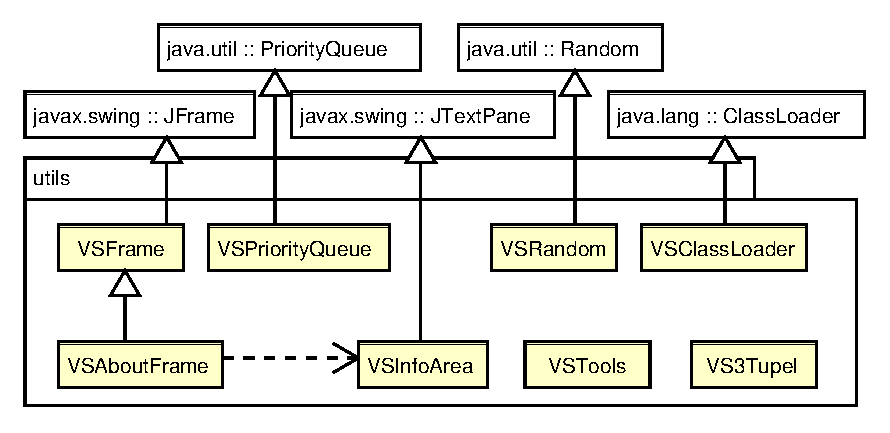
\includegraphics[width=11cm]{images/utils}
	\caption{Das Paket \textit{utils}}
	\label{fig:PackageUtils}
\end{figure}

\begin{itemize}
	\item \textit{VSFrame}: Alle Objekte, die ein eigenes Swing-Fenster besitzen, erben von der Klasse \textit{VSFrame}. Sie stellt sicher, dass neue Fenster an der richtigen Position der Bildf\"{a}che platziert werden und dass Unterfenster (Fenster, die aus einem anderen Fenster aus ge\"{o}ffnet wurden) automatisch mitgeschlossen werden, sobald ihre ``Erzeugerfenster'' geschlossen werden. 
	\item \textit{VSAboutFrame}: Dieses Fenster implementiert die ``About-Anzeige'' die im Simulator \"{u}ber das Datei-Men\"{u} aufgerufen werden kann.
	\item \textit{VSInfoArea}: Ist f\"{u}r die Textanzeige in \textit{VSAboutFrame} zust\"{a}ndig.
	\item \textit{VSClassLoader}: Diese Klasse wird f\"{u}r die automatische Instanzierung von Ereignisobjekten ben\"{o}tigt, wenn dem Simulator lediglich die Klassennamen (aus \textit{events.VSRegisteredEvents}) bekannt sind.
	\item \textit{VSHelper}: In dieser Klasse befinden sich statische Hilfsmethoden, die in keine andere Klasse passen.
	\item \textit{VSPriorityQueue}: Diese Klasse wird f\"{u}r das Verwalten von \textit{core.VSTask}-Objekte im Task-Manager ben\"{o}tigt. \textit{VSPriorityQueue} passt die Priorit\"{a}ts-Warteschlange aus der Java-Standardbibliothek den Anforderungen des Simulators an.
	\item \textit{VSRandom}: Wird f\"{u}r Zufallsereignisse ben\"{o}tigt. Jedes Prozessobjekt besitzt einen solchen eigenen Pseudozufallsgenerator. Diese Klasse setzt gleichzeitig einen eigenen Seed basierend auf der lokalen Systemzeit und anderer Berechnungen fest. 
	\item \textit{VSTupel}: Diese Klasse ist eine Implementierung eines sehr einfach aufgebauten 3-Tupel Datentyps. Alle 3 Elemente k\"{o}nnen von einem anderen Typ sein, was mithilfe der Java-Generics verwirklicht wird. Wird von den Editorklassen f\"{u}r die Generierung von GUI-Elementen ben\"{o}tigt.
\end{itemize}

\begin{figure}[h]
	\centering
	\includegraphics[width=7.5cm]{images/exceptions}
	\caption{Das Paket \textit{exceptions}}
	\label{fig:PackageExceptions}
\end{figure}

Im Paket \textit{exceptions} befinden sich lediglich einige eigene Objekte f\"{u}r Ausnahmebehandlungen. \textit{VSNotCopyableException} wird von einem nicht-kopierbaren Ereignis geworfen, wenn versucht wird es zu kopieren. \textit{VSNegatieNumberException} wird geworfen, wenn intern negative Zahlen dort auftreten, wo sie es nicht sollten. Wenn ein Editorobjekt die Benutzereingabe einer Integer-Vektor-Variable nicht parsen kann, so greifen es auf \textit{VSParseIntegerVectorException} zur\"{u}ck.

\section{Entwicklungsumgebung}

In diesem Teilkapitel soll ein kleiner Einblick in die Umgebung, in der der Simulator entwickelt wurde, gew\"{a}hrt werden. F\"{u}r diese Diplomarbeit wurde ausschlie�lich Open Source Software verwendet. Die einzige Ausnahme stellt Microsoft Windows XP dar, worauf der Simulator zus\"{a}tzlich getestet wurde. Der Simulator wurde jedoch haupts\"{a}chlich unter dem Betriebssystem FreeBSD 7.0, was ein open source Unix-Derivat ist, programmiert. 

Wie bereits bekannt ist, wurde Sun's Java, was mittlerweile auch Open Source Software ist, in der Version 6 (1.6) als die Implementierungssprache gew\"{a}hlt und f\"{u}r die Quelltextdokumentation kam Javadoc und f\"{u}r die automatische Quelltexteinr\"{u}ckung astyle zum Einsatz. Als Built-Tool wurde hier auf Apache Ant gesetzt. F\"{u}r die Erstellung dieses PDF-Dokumentes wurde LaTeX in Verbindung mit dem Built-Tool GNU Make und Rubber verwendet. Eine Rechtschreib\"{u}berpr\"{u}fung wurde mit aspell durchgef\"{u}hrt. xPDF diente als PDF-Anzeigeprogramm.

Als Versionierungssystem wurde SVN (Subversion) verwendet. F\"{u}r den Zugriff auf das SVN-Repository mittels HTTPS (Hypertext Transfer Protocol Secure) wurde der Apache-Websever mit WebDAV-Plugin verwendet. Zudem kam WebSVN als Webschnitstelle des SVN-Repositories zum Einsatz. Als SSL Zertifikat diente ein Kostenloses von CaCert (\url{http://www.CaCert.org}). Mozilla Firefox diente f\"{u}r das Betrachten der Javadocs und der WebSVN-Oberfl\"{a}che.

F\"{u}r schreiben von Java-Quelltext wurde GVim (Graphical Vi IMproved) sowie Eclipse verwendet. Eclipse unterst\"{u}tzt bessere Code-Refactoring-Methoden, w\"{a}hrend GVim mit seiner Flexibilit\"{a}t und schnelleren Editierm\"{o}glichkeiten und mit Vim-Script, der eigenen Script-Engine, gl\"{a}nzt. Es wurden ausserdem das JAutoDoc- (f\"{u}r die Erstellung von Javadoc-Kommentate) und das Subversion-Eclipse-Plugin verwendet. Je nach Zweck wurde zwischen diesen beiden Umgebungen gewechselt. F\"{u}r das Verfassen des LaTeX-Dokumentes wurde GVim verwendet.

S\"{a}mtliche UML-Diagramme wurden mit ArgoUML angefertigt und die Screenshots mit The GIMP (GNU Image Manipulation Program) sowie ImageMagick nachbearbeitet. Mit zip wurden alle VS-Simulator Distributionen eingepackt.

\subsubsection{Linkliste der verwendeten Software}

\begin{itemize}
	\setlength{\itemsep}{-2mm}
	\item Apache Webserver - \url{http://httpd.apache.org}	
	\item ArgoUML - \url{http://argouml.tigris.org}
	\item Eclipse - \url{http://www.eclipse.org}
	\item FreeBSD - \url{http://www.FreeBSD.org}
	\item GNU Make - \url{http://www.gnu.org/software/make}
	\item GVim - \url{http://www.vim.org}
	\item ImageMagick - \url{http://www.imagemagick.org}
	\item Javadoc - \url{http://java.sun.com/j2s2/javadoc}
	\item Mozilla Firefox - \url{http://www.mozilla.com}
	\item Rubber - \url{http://www.pps.jussieu.fr/~beffara/soft/rubber}
	\item Sun Java - \url{http://java.sun.com}
	\item The GIMP - \url{http://www.gimp.org}
	\item WebDAV - \url{http://httpd.apache.org/docs/2.0/mod/mod\_dav.html}	
	\item WebSVN - \url{http://websvn.tigris.org}
	\item aspell - \url{http://aspell.sourceforge.net}
	\item astyle - \url{http://astyle.sourceforge.net}
	\item xPDF - \url{http://www.foolabs.com/xpdf}
	\item zip - \url{http://www.info-zip.org/Zip.html}
\end{itemize}


\chapter{Ausblick}

Es wurde erfolgreich ein Simulator f�r die Simulation verteilter Systeme entwickelt. Der Simulator hat bereits 10 implementierte Protokolle zur Auswahl eingebaut. Zudem steht dem Anwender ein sehr komfortables Protokoll-API zur Verf�gung, womit der Entwicklung neuer Protokolle quasi keine Grenzen gesetzt sind.

Dar�ber hinaus verf�gt der Simulator �ber eine Vielzahl von sehr flexiblen Einstellungsm�glichkeiten. F�r jede Simulation lassen sich somit komplett andere Konfigurationen verwenden. Jeder beteiligte Prozess hat wiederum eigene lokale Einstellungen, wo sich auch jedes Protokoll f�r jeden Prozess separat einstellen l�sst. Die Anzahl und Flexibilit�t der m�glichen Szenarien wird dadurch um einen sehr gro�en Faktor erweitert.

Mit dem Ereigniseditor gibt es eine komfortable M�glichkeit eigene Szenarien zu programmieren um sie anschlie�end zu Simulieren. Hierbei kann entweder auf die bereits enthaltenen Protokolle oder auf selbst implementierte Protokolle zugegriffen werden. Alle dazugeh�rigen Einstellungen und programmierten Ereignisse lassen sich vom Anwender f�r eine sp�tere Wiederverwendung plattformunabh�ngig abspeichern. Somit k�nnen auch abgespeicherte Szenarien beispielsweise an Kommilitonen weitergegeben werden oder f�r eine sp�tere Pr�sentierung zwischengespeichert werden. Durch den Logfilter lassen sich mit Hilfe von regul�ren Ausdr�cken nur die relevanten Lognachrichten anzeigen, was die Analyse einer Simulation erheblich vereinfacht. Weitere Funktionen wie Lamport- und Vektor-Zeitstempel sowie Anti-Aliasing runden den Simulator ab. 

Durch den objektorientierten Aufbau ist der Simulator relativ einfach erweiterbar, was nicht nur das Protokoll-API betrifft. Insgesamt wurde an den meisten Stellen darauf geachtet, dass zu einem sp\"{a}teren Zeitpunkt Erweiterungen einflie�en k\"{o}nnten. Insbesondere soll die Serialisierung von Objekten r\"{u}ckw\"{a}rtskompatibel bleiben, da sonst bei jeder neuen Simulatorversion alle Simulationen erneut angelegt und abgespeichert werden m\"{u}ssten. 

H�tte f�r diese Diplomarbeit noch mehr Zeit zur Verf�gung gestanden, dann h\"{a}tten einige der folgenden Funktionen (hier in alphanumerisch sortierter Reihenfolge aufgelistet) auch Einzug halten k\"{o}nnen:

\begin{itemize}
	\item Die M\"{o}glichkeit Protokolle zu entwickeln ohne den kompletten Quelltext des Simulators vorliegen zu haben. Protokollklassen als separate Bibliothek einzubinden, die dynamisch geladen werden k\"{o}nnen.
	\item Die Simulationsdauer beliebig lang machen zu k�nnen. Dazu m�sste die Klasse \textit{VSSimulatorVisualisation} entlang der Zeitachse scrollbar gemacht werden, so dass der Benutzer f�r eine nachtr�gliche Betrachtung des Simulationsverlaufes zu jeder beliebigen Position zur�ckspringen kann.
	\item Eine Zoomfunktion f�r die Simulationsvisualisierung einzubauen.
	\item Im Ereigniseditor selbst auch periodische Ereignisse programmierbar zu machen. Bisher kann nur jeder Ereigniseintritt separat programmiert werden oder auf Protokoll-Interne Wecker zur�ckgegriffen werden.
	\item Lamport- und Vektor-Zeitstempel als Ereigniseintrittskriterien verwenden zu k�nnen.
	\item Tiefere Schichten des OSI-Referenzmodells simulieren k�nnen, wie z.B. TCP, UDP, IP, ...
	\item Weitere Funktionen einzubauen, wie z.B. das Anklicken einer Nachrichtenlinie, was zu der jeweiligen Nachricht alle verf�gbaren Informationen anzeigt und welche gegebenenfalls vom Benutzer editiert werden k�nnen.
\end{itemize}

Da der Simulator h�chstwahrscheinlich unter einer Open Source Lizenz freigegeben wird, werden die einen oder anderen Funktionen nachtr�glich eingebaut werden. Kommilitonen werden auch herzlich dazu eingeladen sein sich an diesem Software-Projekt zu beteiligen. Als Vorbild sei hier der CPU-Simulator M32 \cite{M32}, der von Prof. O�mann an der Fachhochschule Aachen entwickelt wurde, genannt. Hier existieren bereits einige Erweiterungen und Verbesserungen der Ursprungsversion, die von den Studenten angefertigt wurden. F�r die Entwicklung des VS-Simulators wurde keine propriet�re Software verwendet, so dass jeder kostenlosen Zugriff auf die dazugeh�rigen Tools hat.


\appendix

\chapter{Akronyme}

\begin{acronym}
\acro{API}{Application Programming Interface}
\acro{BSD}{Berkeley Software Distribution}
\acro{GIMP}{GNU Image Manipulation Program}
\acro{GNU}{GNU's Not UNIX}
\acro{GUI}{Graphical User Interface}
\acro{GVim}{Graphical Vi IMproved}
\acro{HTTPS}{Hypertext Transfer Protocol Secure}
\acro{IP}{Internet Protocol}
\acro{JRE}{Java Runtime Environment}
\acro{NID}{Nachrichten-Identifikationsnummer}
\acro{PDF}{Protable Document Format}
\acro{PID}{Prozess-Identifikationsnummer}
\acro{RTT}{Round Trip Time}
\acro{SDK}{Software Development Kit}
\acro{SVN}{Subversion}
\acro{TCP}{Transmission Control Protocol}
\acro{UDP}{User Datagram Protocol}
\acro{VS}{Verteilte Systeme}
\end{acronym}

%\chapter{Akronyms}
\begin{acronym}
\acro{GUI}{Graphical User Interface}
\acro{NID}{Nachrichten-Identifikationsnummer}
\acro{PID}{Prozess-Identifikationsnummer}
\acro{VS}{Verteiltes System}
\end{acronym}


\bibliographystyle{alpha}
\bibliography{bib/references}
%\printindex
\end{document}

%
% EOF
%

